% Define Variables
\newcommand{\gbetitle}{Game Boy Essentials Volume II}
\newcommand{\gbepublishedyear}{2017 - 2023}
\newcommand{\firstpublication}{2019}
\newcommand{\gbeeditionname}{Second Edition}
\newcommand{\gbeISBN}{978-0-9959015-7-5}
\newcommand{\gbededication}{To Annie, for never giving up on me. Even when I’m talking about Game Boy games and you’re trying to sleep.}
% Document Class
\documentclass{book}

% Define Variables
\newcommand{\gbeauthor}{Pierre-Luc Gagné}

% When to Break Words
\hyphenation{Nin-ten-do}
\hyphenation{Mi-ya-mo-to}

% Table Package
\usepackage[table]{xcolor}
\usepackage{tabulary}

% Createspace: createspace.com/Products/Book/InteriorPDF.jsp
% Geometry: texdoc.net/texmf-dist/doc/latex/geometry/geometry.pdf
\usepackage[
paperwidth=5.5in,
paperheight=8.5in,
top=1.5cm,
headheight=3.5mm,
headsep=6mm,
bottom=1.8cm,
footskip=10mm,
inner=2.29cm,
outer=1.52cm,
marginparsep=0cm,
marginparwidth=0cm
]{geometry}

% Fonts Fonts Fonts !
\usepackage{fontspec}
\setmainfont{Adobe Caslon Pro}
\newfontfamily\pageonegbfont[
  SizeFeatures={Size=28}]
  {Early GameBoy}
\newfontfamily\pageoneauthorfont[
  SizeFeatures={Size=20}]
  {Georgia Italic}
\newfontfamily\footerpokefont[
  SizeFeatures={Size=8}]
  {Pokemon GB}
\newfontfamily\pagetwodescription
  {Avenir Next}
\newfontfamily\titlefont[
  SizeFeatures={Size=30}]
  {Avenir Next Ultra Light}
\newfontfamily\htwofont[
  SizeFeatures={Size=20}]
  {Avenir Next Ultra Light}
\newfontfamily\hthreefont[
  SizeFeatures={Size=14}]
  {Avenir Next Demi Bold}
\newfontfamily\codeintextfont[
  SizeFeatures={Size=12}]
  {Inconsolata}
\newfontfamily\dedication[
  SizeFeatures={Size=12}]
  {Georgia Italic}
\newfontfamily\thisgoesintoc[
  SizeFeatures={Size=14}]
  {Avenir Next}

% Left-Align with \begin{flushleft} and \end{flushleft}
\usepackage{ragged2e}
% Line Spacing with \setstretch{1.1}
\usepackage{setspace}
% Hyphenation control
\usepackage{hyphenat}
% Turn off more space after sentences
\frenchspacing
% Have images align to top by default
\raggedbottom
% Set space between paragraphs
\usepackage{parskip}
\setlength{\parskip}{0.8em}
\setlength{\parindent}{1.5em}

% Image Package
\usepackage{graphicx}
\usepackage{float}
\graphicspath{ {book-assets/} }
\usepackage{wrapfig}
\usepackage{adjustbox}
\usepackage{placeins}

% List item package
\usepackage{enumitem}

\let\oldcenter\center
\let\oldendcenter\endcenter
\renewenvironment{center}{\setlength\topsep{0pt}\oldcenter}{\oldendcenter}

% Page Details
% Show wireframes for development
%\usepackage{showframe}

% Define Chapters
\usepackage{needspace}
\usepackage{titlesec}
\titleformat{name=\chapter}[block]{\titlefont\raggedright\setstretch{3}}{}{0pt}{}[]
\titlespacing{name=\chapter}{0pt}{-30pt}{6pt}[0pt]
\titleformat{name=\section}[block]{\htwofont\raggedright\setstretch{2}}{}{0pt}{}[]
\titlespacing*{name=\section}{0pt}{10pt}{0.4em}[0pt]
\titleformat{name=\subsection}[block]{\hthreefont\raggedright\setstretch{1.8}}{}{0pt}{}[]
\titlespacing*{name=\subsection}{0pt}{4pt}{0.4em}[0pt]

% Table of Contents
\usepackage{titletoc}
\renewcommand{\contentsname}{Table of Contents}
\titlecontents{chapter}[0pt]{\thisgoesintoc}
{\thecontentslabel\enspace}
{}
{\titlerule*[4pt]{.}\raggedright\contentspage}[\vskip 7pt]

% Headers & Footers
\usepackage{fancyhdr}
\fancyhf{} % sets both header and footer to nothing
\renewcommand{\headrulewidth}{0pt}
\pagestyle{fancy}
\renewcommand{\chaptermark}[1]{\markboth{#1}{}}
\lhead[]{}
\chead[]{}
\rhead[]{}
\lfoot[\footerpokefont \thepage]{\pagetwodescription \leftmark}
\cfoot[]{}
\rfoot[]{\footerpokefont \thepage}

\fancypagestyle{plain}{
\fancyhf{}
\fancyfoot[R]{\footerpokefont \thepage}}

% Making printing compliant PDF
%\usepackage[x-1a]{pdfx}

% Begin Document
\begin{document}
\begingroup
\setlength{\columnsep}{1.7mm}
\setlength{\intextsep}{0mm}

\thispagestyle{empty}
\mbox{}
\vskip 70pt
\begin{flushleft}
\setstretch{4}
\pageonegbfont \nohyphens{\gbetitle{} \par}
\setstretch{3}
\pageoneauthorfont \nohyphens{by \gbeauthor{} \par}
\end{flushleft}
\vfill
\newpage

\thispagestyle{empty}
\mbox{}
\vfill
\begin{center}
\setstretch{1}
\fontsize{10pt}{12pt}\selectfont
\pagetwodescription {\gbetitle{}\par © \gbepublishedyear{} by Pierre-Luc Gagné\par \vskip 9pt gameboyessentials.com \vskip 9pt \gbeeditionname{}\par \vskip 9pt This book is set in Adobe Caslon Pro, with Inconsolata for monospaced segments, and Avenir Next for headings. It also uses fonts from {\em Super Mario Land} and {\em Pokémon} for flourishes. \vskip 9pt ISBN \gbeISBN{}\par \vskip 9pt The copyright for game boxes and screenshots reproduced in this book remain with the respective owners of those works.}
\end{center}
\newpage

\thispagestyle{empty}
\mbox{}
\vfill
\begin{raggedleft}
\setstretch{1.1}
\dedication{\gbededication{}}
\vfill
\end{raggedleft}
\newpage

\begingroup
\let\cleardoublepage\clearpage
\tableofcontents
\endgroup
\thispagestyle{empty}
\fontspec{Adobe Caslon Pro}[WordSpace = 1.1]
%\fontspec{Adobe Caslon Pro}
%\addfontfeature{LetterSpace=1.0}
\setstretch{1.2}
\fontsize{12pt}{12pt}\selectfont\begingroup \chapter*{Introduction}\markboth{Introduction}{}\addcontentsline{toc}{chapter}{Introduction} \endgroup
This book is the second volume of Game Boy Essentials, an attempt to understand the Game Boy library through its essential titles, good or bad. I have always looked forward to self-publishing this second book more than the first one, even before I started the project.

You see, I think anybody can write one book. I honestly believe that anyone who sets their mind to it can write something and use the tools available for free to self-publish. What is tough is publishing a second book; the novelty of saying you’re writing a book is gone. It took me much longer than I planned to write the twelve articles you see in this book. I had fully expected my excitement to recede. I knew, even before I started writing the first volume, that the second one would be the difficult achievement.

Do not mistake me; I am ultimately very happy with the written words in this book. I believe the twelve articles you hold in your hands are my best articles so far. I just had a harder time finding the motivation to write them. One thing was still exciting and required little motivation, however: typesetting.

When you typeset a book, you end up discovering if you like doing it. And most people don’t like paying attention to what needs to happen to create a book. I discovered I loved it. Not necessarily that I was any good at it, but that I had a lot of fun stressing all the little minutiae that goes into making the physical thing that is a book. What book size do you feel works best with your content? What font do you use? What about line height? Etc.

Typesetting my first book was also a mess. Because I wanted the process to be straightforward, my first book was made using Apple’s Pages. It speaks to the power of this application that I was able to make it using its limited tool set. Unfortunately, the amount of time and effort it took to manually place every image and arrange every paragraph was simply too time-consuming to joyfully repeat for my second book. Pages also has some severe functionality gaps with page layout. My improved skills in programming came to my rescue. Last year, I had switched the management of my website to Jekyll. Gameboyessentials.com was previously hand-crafted, with more and more automated shell scripts written by me over time to automate tasks until it became unwieldy. Jekyll changed that for the better. It’s a wonderful static site generator that I was able to mould into making my idiosyncratic website. It’s extremely popular and well documented, so I was quickly able to find solutions to all my problems. I didn’t need any strange hack, I simply used its Collections feature to code all the details I wanted. Once that project was completed, and I could manage my site with ease, I was itching for more coding challenges. That’s when I looked at my book.

Before I even dabbled in Jekyll, I had tried automating the typesetting of my book with ConTeXt, a variant of TeX focused on separating your styling from your text. Unfortunately, ConTeXt failed me. I am not a professional programmer. Stack Overflow taught me everything I know. ConTeXt had so little documentation that I had to abandon my endeavour; I simply could not find answers to very basic questions. That’s when I turned to Pages and ended up with the first edition of my first book. I luckily decided to give the TeX family a second chance once my website was updated, a couple of months later. Using Jekyll made me realize that my problem with ConTeXt was with its anemic documentation. So I tried building my book with LaTeX, the most popular flavour of TeX. If you’re an academic outside the humanities, you’re bound to know what LaTeX is. If not, it’s a typesetting system that works using plain text with markup to style your finished document. It’s code. Most research papers who need to show mathematical equations are built using LaTeX because of its foolproof nature. Look at this example of my book’s legal notice page.

\noindent{\codeintextfont 
\noindent{\codeintextfont
\textbackslash thispagestyle{empty}
\newline \textbackslash mbox{}
\newline \textbackslash vfill
\newline \textbackslash begin{center}
\newline \textbackslash setstretch{1}
\newline \textbackslash fontsize{10pt}{12pt}\textbackslash selectfont
}
}

This short example allows the page to be bottom-aligned. Using a system based on such markup, I was able to convert my website’s HTML into LaTeX using a mixture of Ruby and Bash scripts. I would look for specific HTML tags for my images, my chapter titles and so forth and convert them into the corresponding LaTeX markup. I quickly learned that you’re not supposed to do that in a professional setting with other people’s HTML. But since every line was written by me, I had no qualm about parsing my own HTML. The final LaTeX code might be messy and weird, but it didn’t matter; the final PDF looked like what I wanted. It took a while to code for every possible permutation on my website, but it was worth it. I finally switched to XeLaTeX since it allowed me to use modern font files. This book is actually the second book I’ve made using my Jekyll, Bash, Ruby and XeLaTeX workflow: my initial project involved redoing the first volume, which features my first twelve articles. I stealthily republished it in a fancy second edition. The text is lightly edited, and if you don’t pay too much attention you won’t see the typesetting differences. But I do.

I seem to be forgetting, dear reader, that you’re not here for bookmaking nerdery, but rather for Game Boy analysis. Fortunately, the rest of this book is all about that. The twelve following articles cover a fascinating tranche of video games, representing a large swath of what the Game Boy represented.

Enjoy.




























\begingroup \chapter*{Matchbox Caterpillar Construction Zone}\markboth{Matchbox Caterpillar Construction Zone}{}\addcontentsline{toc}{chapter}{Matchbox Caterpillar Construction Zone} \endgroup
\begin{figure}[H]
\vskip 4pt
\centering
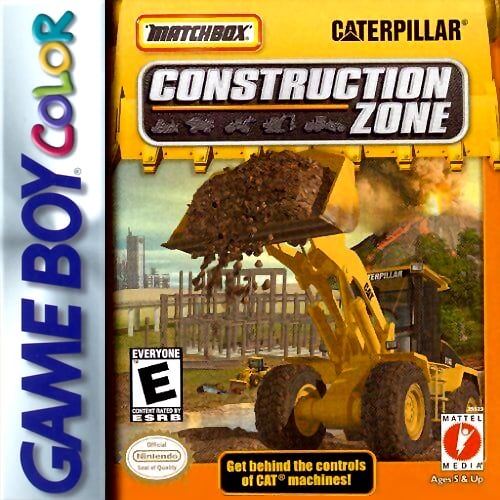
\includegraphics[width=.75\linewidth]{assets/assets/dmg-ar4e/dmg-ar4e-1.jpg}\end{figure}
\begin{itemize} [nosep]




\item North American release in January 2000







\item European release in 2000








\item Never released in Japan





\item Developed by Realtime Associates

\end{itemize}\noindent

\newpage\FloatBarrier\needspace{10mm}\section*{Honk! Honk!}\nopagebreak[4]
\begin{wrapfigure}{L}{0pt} 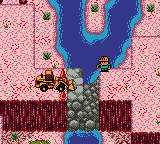
\includegraphics[width=.45\linewidth]{assets/assets/dmg-ar4e/dmg-ar4e-2.png}\end{wrapfigure}
The Game Boy was going through a frenzy of popularity in 2000. What do I mean by a frenzy? People were buying a large number of games for the system, making it viable to develop more games for the system. Any type of game could find an audience.

During the continuing success of \emph{Pokémon} and after the release of the Game Boy Color, it was a good deal for a developer to grab a franchise, make a Game Boy game with Game Boy Color support (a black cartridge) and just see what sticks. To me the best example of this era of 1999–2000 Game Boy Color games is best represented by \emph{Matchbox Caterpillar Construction Zone}. Why? Because I friggin’ bought the game at retail with hard-earned teenager money, that’s why! For what reason did I buy this game? I still don’t know to this day. But I’m familiar with it and so I can talk about it. It’s not the only game you could use to represent this era but for me the boomtown mentality of 1999–2000 on Game Boy is best portrayed by \emph{Matchbox Caterpillar Construction Zone}.

\FloatBarrier\needspace{10mm}\section*{Humble Roots}\nopagebreak[4]

\emph{Construction Zone} was originally a PC game. A kids game about driving large machinery, it came with a set of controls you could stick on top of your keyboard to pretend you were in a big truck, or a big bulldozer, or whatever!

\begin{figure}[hbt]
\vskip 10pt
\centering 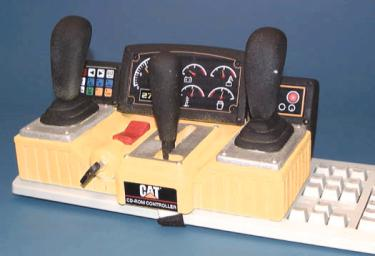
\includegraphics[width=.5\linewidth]{assets/assets/dmg-ar4e/dmg-ar4e-3.jpg}
\vskip 6pt
\end{figure}
The joystick really defines what these types of games hoped to achieve. It looks good in the ad, and above all it’s meant to be dead simple to set up for kids. The controller mechanically connects to your computer keyboard, so movements on the controller move levers that push keyboard buttons. No need to install drivers or mess with DLLs to configure this Windows~95 peripheral! The whole project feels more like a toy than proper software. Makes sense when the game has the name Matchbox in the title.

\begin{wrapfigure}{L}{0pt} 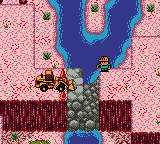
\includegraphics[width=.45\linewidth]{assets/assets/dmg-ar4e/dmg-ar4e-4.png}\end{wrapfigure}
So you had this \emph{PC toy} coming out and somehow it made financial sense to have a Game Boy version come out as well. I find it fascinating that nine people are credited with making a goddamn construction simulator on Game Boy. Who are these people? What do they think of their game? I can’t help but wonder: How much time did they spend making this game? Some of those credits are for executive producers, sure, but the game had three programmers and a sound person. They probably worked on this project for months. As an aside, some of the personnel on this game also worked on \emph{Heroes of Might \& Magic} on Game Boy Color. I guess assembly programmers versed in Game Boy minutia were not around every corner.

\FloatBarrier\needspace{10mm}\section*{The Down Low}\nopagebreak[4]

There is not a lot to say about \emph{Matchbox Caterpillar Construction Zone}. You can’t lose, you can’t get screwed, you just have to perform the very simple actions the game requires and that’s it. You could expect a sandbox where you get to do whatever you want with the big machinery but the game is frustratingly story-driven. There’s no way to cause any fun mayhem. You just follow the steps as they are presented by the game. One thing that caught my eye is how little text there is. Since this is ostensibly a game for kids, you’d expect a healthy dose of tutorials. This is not the case. The game uses the very ingenious device of a little foreman simply pointing you in the right direction when you’ve finished a task.

\begin{figure}[hbt]
\vskip 10pt
\centering 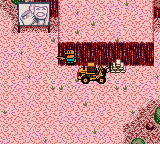
\includegraphics[width=4.85cm]{assets/assets/dmg-ar4e/dmg-ar4e-5.png}
\vskip 6pt
\end{figure}
Why go to all the trouble of animating this little character when a text field would have been much simpler? I think it’s a case of building something without text so you don’t have to translate it later. I found it interesting. It gives the game personality and it’s fun to see the little foreman disapprove when you do the wrong thing. It shows how cheapo releases can still show some amount of effort and ingenuity.

\begin{figure}[hbt]
\vskip 10pt
\centering 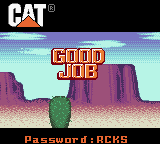
\includegraphics[width=4.85cm]{assets/assets/dmg-ar4e/dmg-ar4e-6.png}
\vskip 6pt
\end{figure}
In terms of mistakes and missed opportunities I think the game suffers the most from its ginormous maps. You often get lost and with the complicated tank controls it’s hard to move around. You should have tank controls to make you feel like you’re operating very big machines but these controls are jerky so you never feel like you’re driving a big vehicle. It would have been better if you had a control scheme based on large archs to maneuver the machines around tight corners and smaller areas. To top it off they maybe could have included an HP meter to limit the number of times you could drive into stuff. I feel like that’s probably the main concern when operating a bulldozer; don’t bump into things. Here your main concern is not to get lost on the way to the fourth rock you need to move.

\FloatBarrier\needspace{10mm}\section*{Realtime Associates, Inc.}\nopagebreak[4]

\begin{figure}[hbt]
\vskip 10pt
\centering 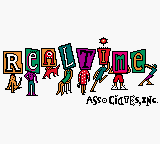
\includegraphics[width=4.85cm]{assets/assets/dmg-ar4e/dmg-ar4e-7.png}
\vskip 6pt
\end{figure}
Ultimately, \emph{Matchbox Caterpillar Construction Zone} is terribly unimportant. The company’s own website lists the game under the wrong name, for chrissake. Realtime Associates’ history is interesting though: they were created out of a bunch of Intellivision developers and made the NES port of \emph{Maniac Mansion} and \emph{Bug!} for the Sega Saturn, along with a dizzying number of licensed games. Go read more about their history on their About Page. To me, they’ll always be the developer of \emph{Out of Gas} for Game Boy, which I’ll get to in due time.

\FloatBarrier\needspace{10mm}\section*{Conclusion}\nopagebreak[4]

\begin{wrapfigure}{R}{0pt} 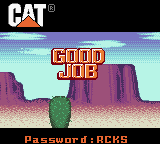
\includegraphics[width=.45\linewidth]{assets/assets/dmg-ar4e/dmg-ar4e-8.png}\end{wrapfigure}
I think I’ve already proven with both \emph{Heroes of Might \& Magic} that I’m not scared to highlight really surprising games. \emph{Construction Zone} is such a game. It’s easy crap for kids, but it shows that in 1999–2000 there was a market for those games. Compare what was released for Game Boy Color in 2000 with was released for Game Boy in 1997. See a difference? In 1997, the Game Boy was winding down because nobody cared anymore. In 2000, developers were still trying to reap the spoils of a tsunami that reinvigorated the Game Boy: \emph{Pokémon}. That’s why \emph{Matchbox Caterpillar Construction Zone} was made and that’s why it’s essential. It shows you a gold rush in full swing.

\begin{figure}[hbt]
\vskip 10pt
\centering 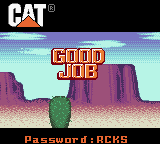
\includegraphics[width=4.85cm]{assets/assets/dmg-ar4e/dmg-ar4e-9.png}
\vskip 6pt
\end{figure}



\begingroup \chapter*{The Bugs Bunny Crazy Castle}\markboth{The Bugs Bunny Crazy Castle}{}\addcontentsline{toc}{chapter}{The Bugs Bunny Crazy Castle} \endgroup
\begin{figure}[H]
\vskip 4pt
\centering
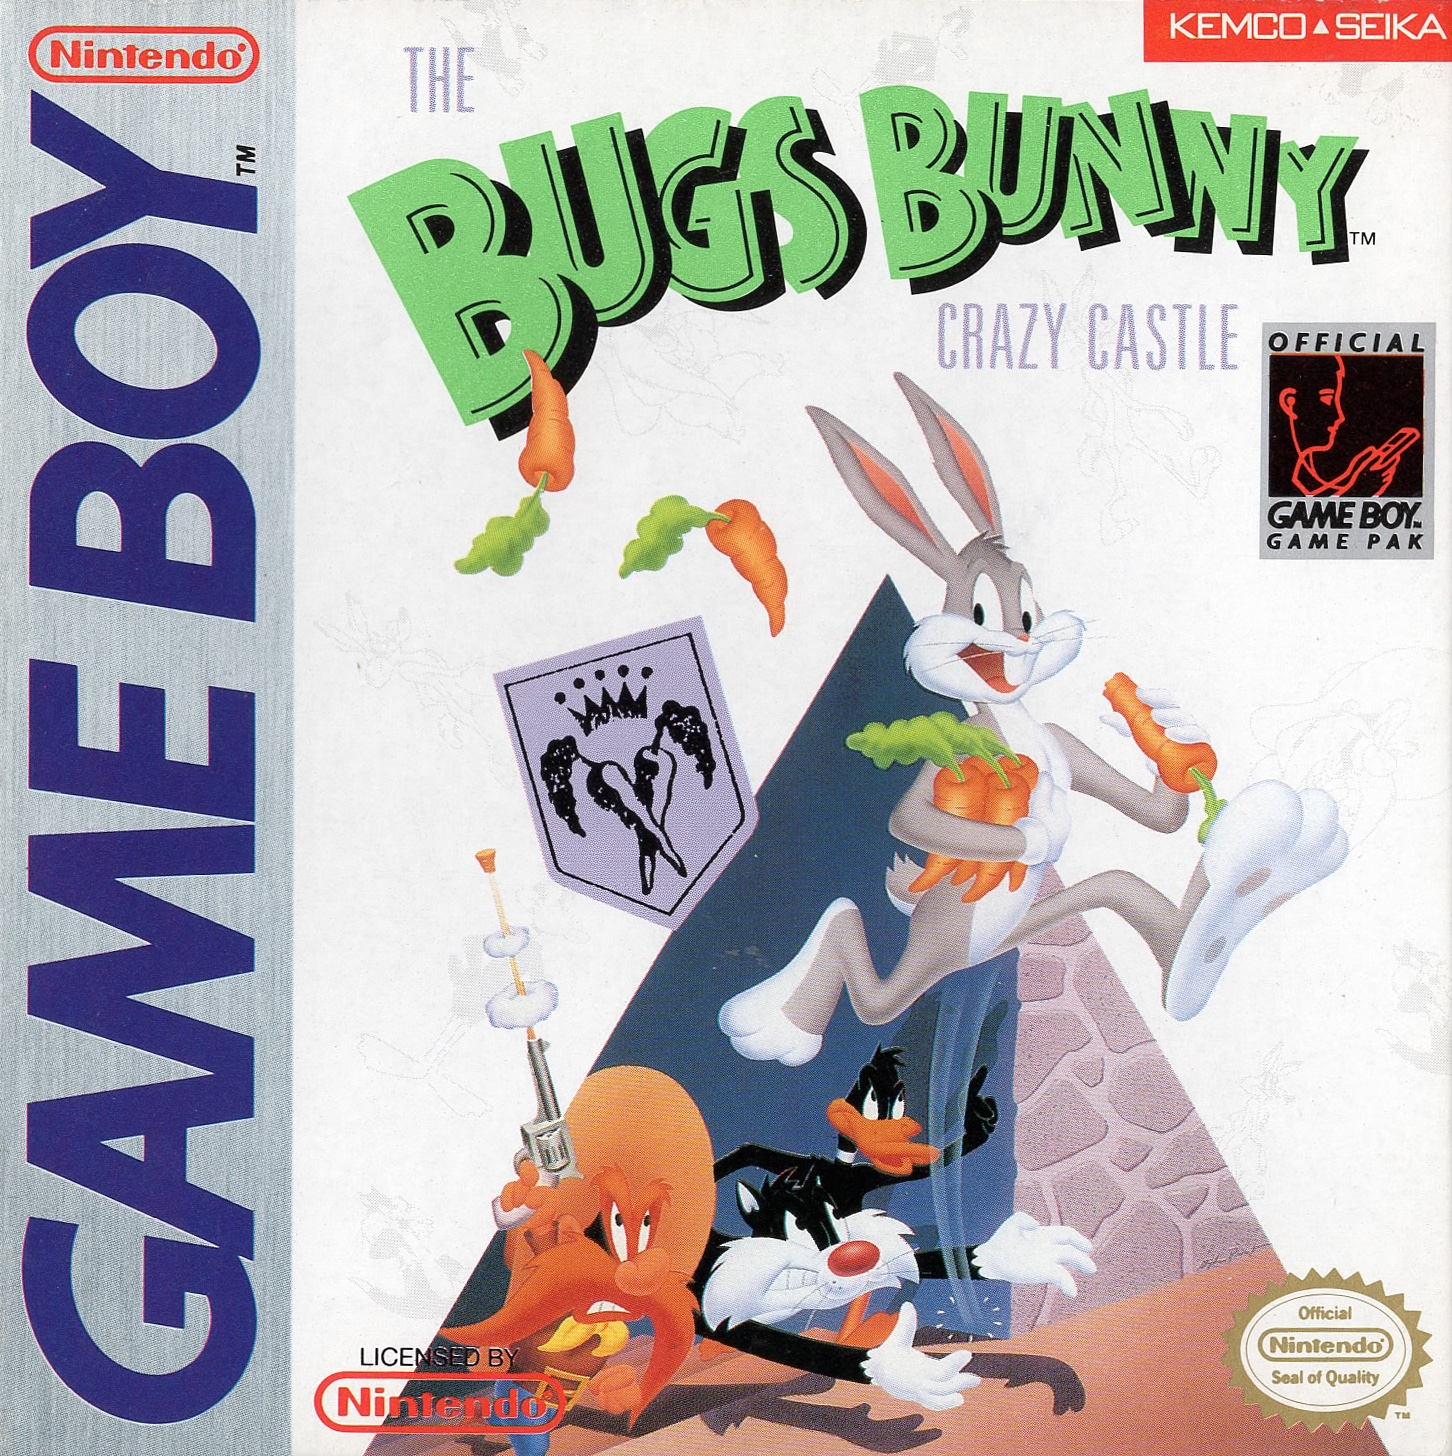
\includegraphics[width=.75\linewidth]{assets/assets/dmg-bb/dmg-bb-1.jpg}\end{figure}
\begin{itemize} [nosep]




\item Japanese release in September 1989







\item North American release in March 1990







\item European release in 1990







\item North American release in 1998
\begin{itemize} [nosep]\item Player’s Choice\end{itemize}\noindent











\item Developed by Kemco

\end{itemize}\noindent

\newpage\FloatBarrier\needspace{10mm}\section*{Crazy Stupid Love}\nopagebreak[4]
\begin{wrapfigure}{L}{0pt} 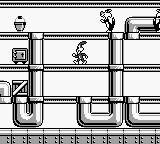
\includegraphics[width=.45\linewidth]{assets/assets/dmg-bb/dmg-bb-2.png}\end{wrapfigure}
I hate Kemco’s \emph{Crazy Castle} series. It’s not fun or interesting. It also has one of the most complicated release history around. But we must talk about the first game released on Game Boy. Why? Because it’s the first Game Boy title to do two things:

\begin{enumerate}
\item It is the first \emph{action} title to feature large sprites;
\item It is arguably the first multi-platform release, being made available on NES and Game Boy, albeit with different levels.
\end{enumerate}\noindent

It struck a chord with the public and sold more than a million copies. Being an early release certainly helped; it had little competition and featured a very well-known licensed character. A whole bunch of future titles would do the exact same thing, but \emph{The Bugs Bunny Crazy Castle} was the first. For that, and certainly not for its brain-dead gameplay, it’s essential.

It was eventually rereleased as a Player’s Choice title in 1996 (that’s the only way I know it sold more than a million copies) at the nadir of the Game Boy’s history, giving the game a second life.

\FloatBarrier\needspace{10mm}\section*{The Meandering Story of Its Rotating Cast of Franchises}\nopagebreak[4]

Kemco gets the right to make a Roger Rabbit game for the Famicom Disk System. So far, so good. They create the game and release it in February of 1989, six months after the movie is released in the US but just two months after the release in Japanese theatres in December of 1988. The timing is so tight it’s possible they started developing the game as a blank slate before they had a franchise to put on the game.

\begin{center}
\quad\vspace{4pt}\adjustbox{valign=t}{ \sbox0{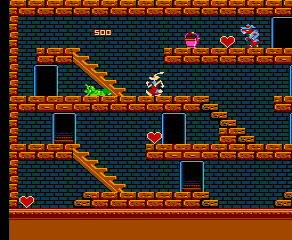
\includegraphics[width=.45\linewidth]{assets/assets/dmg-bb/dmg-bb-3.png}}\begin{minipage}[t]{\wd0}\usebox0\par\centering\pagetwodescription Roger Rabbit\end{minipage}}
\quad\vspace{4pt}\adjustbox{valign=t}{ \sbox0{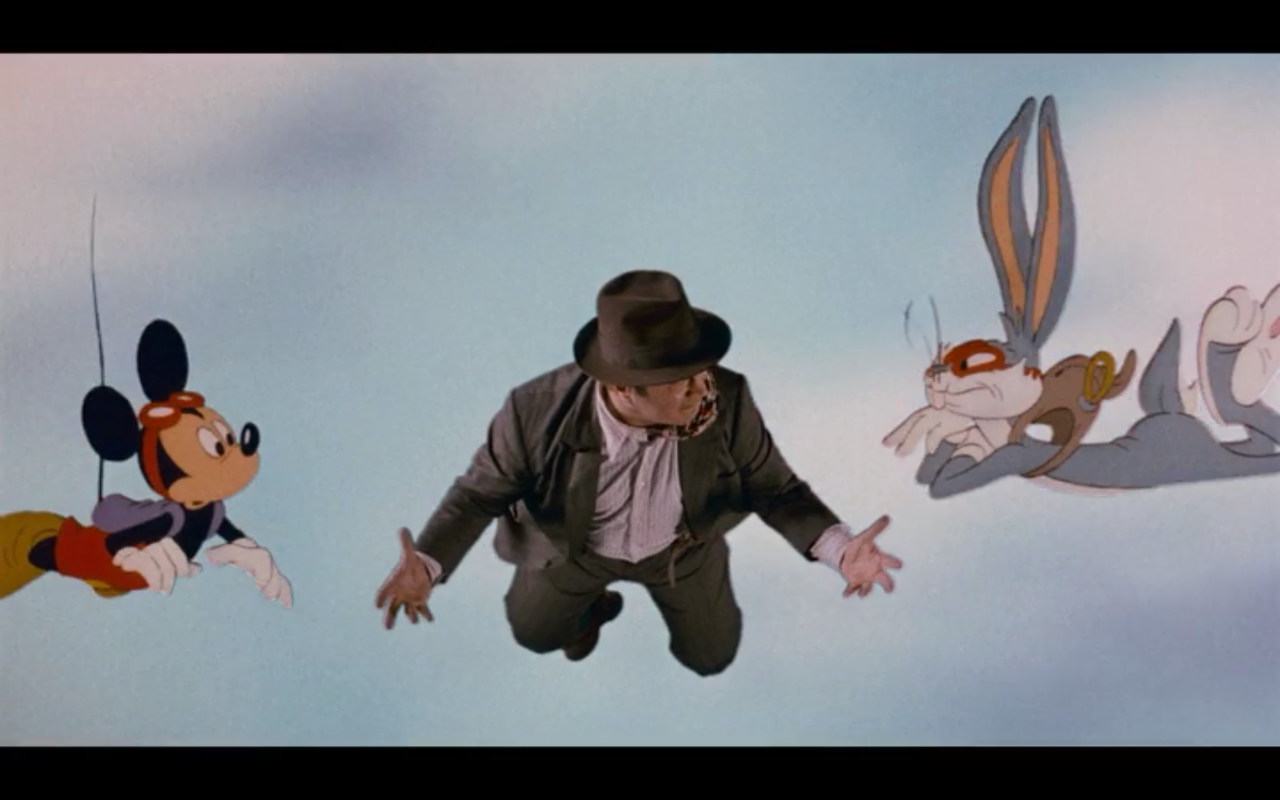
\includegraphics[width=.45\linewidth]{assets/assets/dmg-bb/dmg-bb-4.png}}\begin{minipage}[t]{\wd0}\usebox0\par\centering\pagetwodescription Bugs Bunny\end{minipage}}
\end{center}
Now comes the time to get your throwaway game to North America. But in North America, Kemco did not hold the video game rights for the \emph{Roger Rabbit} movie. Another game based on \emph{Who Framed Roger Rabbit} was instead released to coincide with its VHS release, a really big event back in the fall of 1989. It’s not the same game as the Japanese one: it was published by LJN and developed by Rare of all people. Kemco did release its game in North America, but as \emph{The Bugs Bunny Crazy Castle}. They ported the game to cartridge (from an FDS diskette) and changed the sprites into Looney Tunes characters. How did we end up in this situation?

It’s not necessarily a simple answer of LJN having snatched the rights in North America before Kemco could localize their version. It’s very possible that Kemco being a Japanese company, they concentrated on getting the game out in Japan without ever really thinking about a worldwide release. It might be possible that Kemco did not think it was worth paying for the rights to a movie out of American theatres, and they did not consider coinciding their game with a VHS release. It might be possible that the movie being a big hit, the price for the rights went up and shut out Kemco. It might be possible that the game being out, the American rights holder saw the Japanese version and thought it was inappropriate. I don’t know. The rights to Roger Rabbit himself are convoluted, to say the least; Spielberg has to this day a veto on anything Roger Rabbit related (the movie version of the character: Roger Rabbit was adapted from a novel), we can only presume at the complicated discussions that left us with the situation we’re in with the \emph{Crazy Castle} games.

\begin{wrapfigure}{L}{0pt} 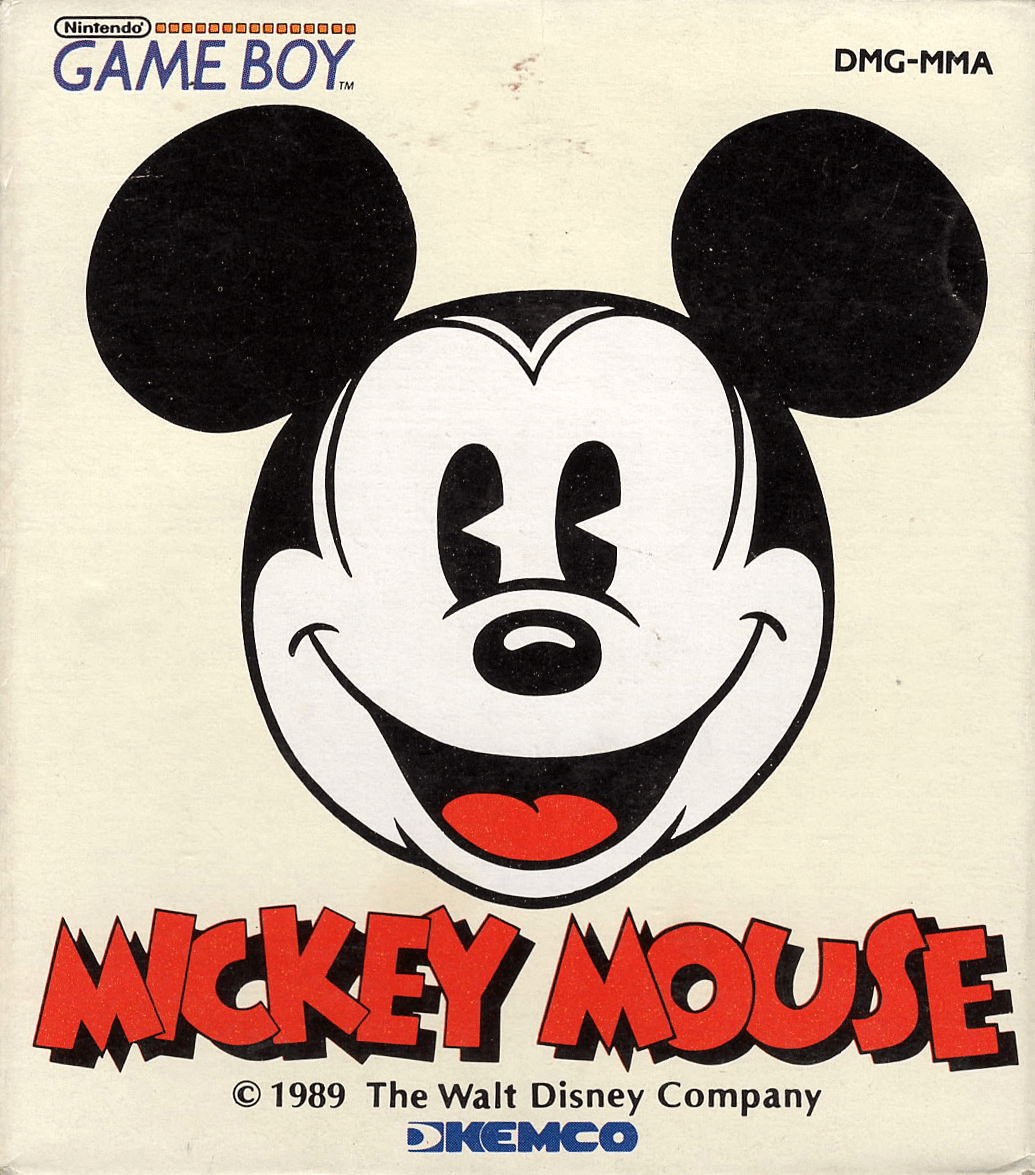
\includegraphics[width=.4\linewidth]{assets/assets/dmg-bb/dmg-bb-5.png}\end{wrapfigure}
Kemco seemed to have had the avant-garde idea of releasing a version of their Famicom/NES game for the portable Game Boy. Nobody had done that on Game Boy before. \emph{Tennis} \& \emph{Baseball} by Nintendo were adaptations of old Famicom sports titles. \emph{Hyper Lode Runner}, which came out in Japan a couple of weeks after Kemco’s game was a new version of an old PC title. But a contemporary licensed game, released on Nintendo’s two consoles around the same time, that was still new ground. So we have the Japanese release in the fall of 1989 of \emph{Mickey Mouse} for Game Boy. Wait a minute? Wasn’t this article about \emph{The Bugs Bunny Crazy Castle}? Where does Mickey Mouse come into play? Kemco did not have the same licence in different regions, so they just changed the licensed characters in their games. See this handy chart:

\begin{center} \footnotesize\begin{tabulary}{\textwidth}{LLLL} \hline
\textbf{Japanese Release} & \textbf{North American Release} & \textbf{European Release} & \textbf{Comments} \\
\hline
\emph{Roger Rabbit} & \emph{The Bugs Bunny Crazy Castle} & Not released & The original FDS version and the NES adaptation. \\
\hline
\emph{Mickey Mouse} & \emph{The Bugs Bunny Crazy Castle} & \emph{The Bugs Bunny Crazy Castle} & The game we are talking about here: it’s really a sequel, not a port of the previous game. \\
\hline
\emph{Mickey Mouse II} & \emph{The Bugs Bunny Crazy Castle~2} & \emph{Hugo} or \emph{Mickey Mouse} & The second Game Boy game, third overall; by the way, who the hell is Hugo? \\
\hline
\emph{Mickey Mouse III: Balloon Dreams} & \emph{Kid Klown in Night Mayor World} & Not released & A late NES platformer, only considered in the series because of its Japanese numbering. \\
\hline
\emph{Mickey Mouse IV: The Magical Labyrinth} & \emph{The Real Ghostbusters} & \emph{Garfield Labyrinth} & Back to Game Boy, with every market having a different licence! Oh boy! \\
\hline
\emph{Mickey Mouse V: The Magical Stick} & \emph{Mickey Mouse: Magic Wands!} & \emph{Mickey Mouse V: Zauberstaebe!} & A Game Boy release, it sold a million copies in North America and got rereleased in 1998. It shows how strong the Mickey Mouse brand is. \\
\hline
\emph{Let’s Go!! Kid: Go! Go! Kid} & Not released & Not released & They clearly no longer had the Mickey Mouse licence. It released without any licence attached. \\
\hline
\emph{Bugs Bunny: Crazy Castle~3} & \emph{Bugs Bunny: Crazy Castle~3} & \emph{Bugs Bunny: Crazy Castle~3} & A Game Boy Color enhanced version of \emph{Go! Go! Kid}; it renumbered the series in Japan and picked up Bugs Bunny for every market. \\
\hline
\emph{Bugs Bunny in Crazy Castle~4} & \emph{Bugs Bunny in Crazy Castle~4} & \emph{Bugs Bunny in Crazy Castle~4} & A Game Boy Color only release. \\
\hline
\emph{Woody Woodpecker in Crazy Castle~5} & \emph{Woody Woodpecker in Crazy Castle~5} & \emph{Woody Woodpecker in Crazy Castle~5} & A GBA game, it seems they lost the Bugs Bunny licence and went with something cheaper. Woody Woodpecker is not a hot licensing opportunity. \\
\hline \normalsize\end{tabulary} \end{center}

So we have a game series that started out as a somewhat hard FDS \emph{Roger Rabbit} cash-in that became an easier series of Game Boy \emph{Mickey Mouse} games in Japan re-skinned as \emph{The Bugs Bunny Crazy Castle} in North America. It’s all fitting, considering Bugs and Mickey both appeared in \emph{Roger Rabbit}. ~

\begin{figure}[hbt]
\vskip 10pt
\centering 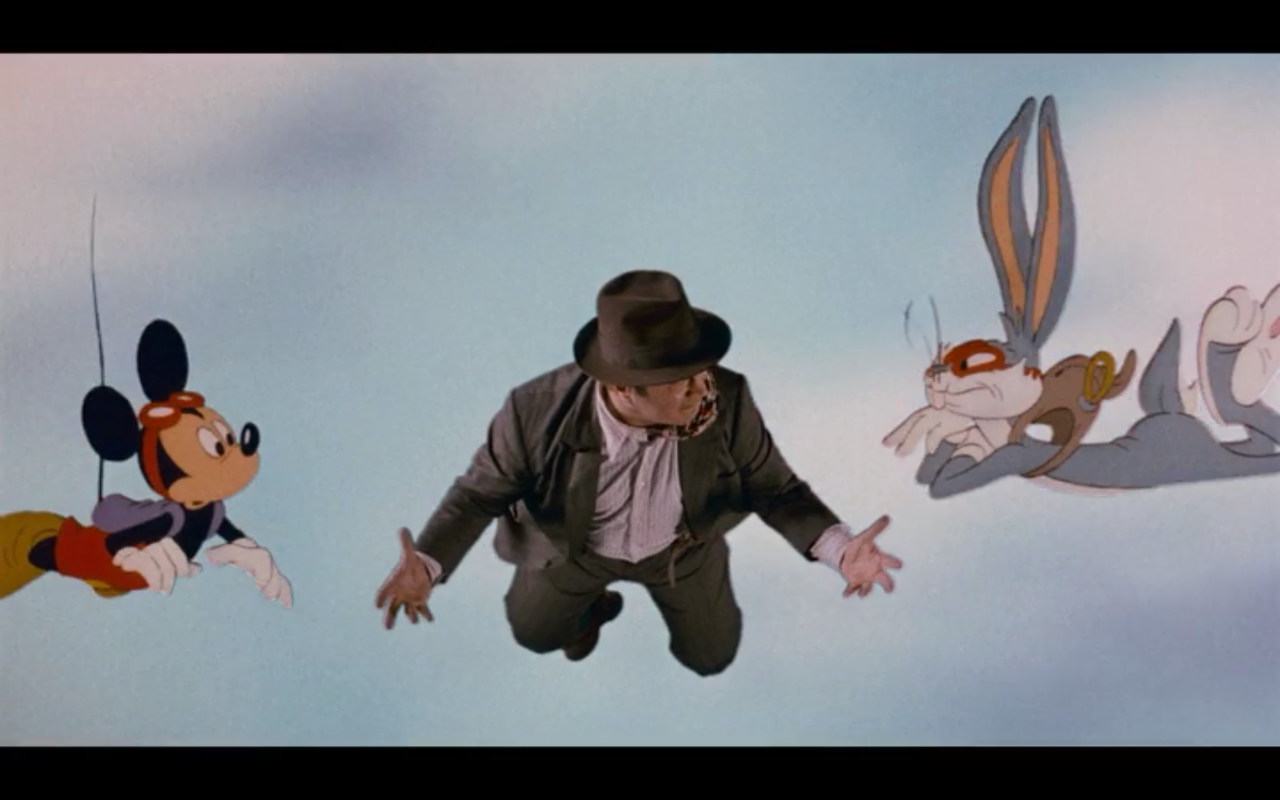
\includegraphics[width=.75\linewidth]{assets/assets/dmg-bb/dmg-bb-6.png}\par\pagetwodescription You’d think Kemco would re-skin the \emph{Crazy Castle} games with Bob Hoskins in Australia or something.
\vskip 6pt
\end{figure}

\FloatBarrier\needspace{10mm}\section*{Lode of Crap}\nopagebreak[4]

\begin{figure}[hbt]
\vskip 10pt
\centering 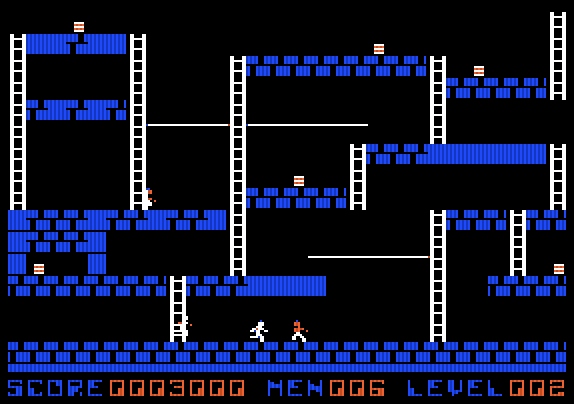
\includegraphics[width=.6\linewidth]{assets/assets/dmg-bb/dmg-bb-7.png}\par\pagetwodescription The Apple ][ version
\vskip 6pt
\end{figure}
\emph{Roger Rabbit}, and thus the whole \emph{Crazy Castle} series, is basically a ripoff of \emph{Lode Runner}. A game by Douglas E. Smith, \emph{Lode Runner} was released on microcomputers in 1983, and published by Brøderbund. You’re a stick figure, running around in a side view labyrinth of platforms and ladders, with the objective of gathering all the gold strewn around the level to move on. But beware the enemy stick figures that walk around! You have no way of defeating them; your only tool against them are holes you can dig to stop them for a very short time. This allows you to walk over their head and continue along your path. It’s a platformer of its time, made well before \emph{Super Mario Bros.} changed everything: you have to get really intimate with its AI mechanics to achieve any kind of success. Play it today and you’ll be wishing for a jump button after one level. What is interesting for us is the Hudson Soft port for Famicom released in 1984. It featured different, larger levels with scrolling since the Famicom could smoothly scroll while microcomputers couldn’t. It introduced no new concepts to the game, still featuring a character moving across a side view labyrinth in search of gold, digging holes to temporarily stop his enemies. The Family Computer (the Japanese version of the NES) had a dearth of releases for its first two years on the market but was very successful as a console. Nintendo was kind of caught with their pants down. So a game like \emph{Lode Runner}, which in all honesty is not that fun, sold \textbf{millions} of copies in Japan and became a beloved classic even though its kind-of terrible. The best comparison I have is to the first NES \emph{Teenage Mutant Ninja Turtles} game and its revered status here in North America. It’s bad, we all know it’s bad, but we played it too much \textbf{not} to love it. Sometimes love is illogical.

\begin{figure}[hbt]
\vskip 10pt
\centering 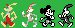
\includegraphics[width=.6\linewidth]{assets/assets/dmg-bb/dmg-bb-8.png}
\vskip 6pt
\end{figure}
\emph{Roger Rabbit} on FDS is an extension of the concept of \emph{Lode Runner}. You run around for hearts in each level instead of gold, it replaces ladders and tightropes with staircases and pipes, and instead of digging holes to defeat your enemies you push 100-ton weights on them or throw punching gloves. Just like the cartoons! Once hit, enemies disappear for good in a puff of smoke, making \emph{Crazy Castle} much more manageable than \emph{Lode Runner’s} pacifist brand of gameplay. Even with those changes, \emph{Roger Rabbit} on FDS is not an easy game. It’s easier than \emph{Lode Runner}, but it’s still a mean game. Japanese audiences would have been accustomed to it though; they had years of \emph{Lode Runner} derivatives under their collective belt in 1989. In North America we saw most of those games but they were never popular. This meant we were collectively not used to this brand of gameplay. So \emph{The Bugs Bunny Crazy Castle} on NES made one big concession: the enemies are slower.

\begin{wrapfigure}{L}{0pt} 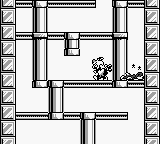
\includegraphics[width=.45\linewidth]{assets/assets/dmg-bb/dmg-bb-9.png}\end{wrapfigure}
We now get to our game of interest: the Game Boy version. You might be tempted to think it’s a straight port with the same levels, but it’s not. It’s more akin to a sequel. It has the same mechanics (staircases, punching gloves and 100 ton weights) but new levels. The graphics are also redrawn and are honestly much better looking than on NES. Remember that we have two versions of the game: the Japanese \emph{Mickey Mouse} and the North American version. I’ve looked carefully and I do not see any difference between the Japanese \emph{Mickey Mouse} and the North American \emph{Bugs Bunny} (except for the whole Mickey Mouse thing, obviously). So both games are much easier in enemy placement, much simpler in level design than the previous FDS/NES games and that was considered sufficient to please everyone. So the only difference between both Game Boy releases is a simple palette swap, which will become this forsaken series’ best remembered characteristic: palette swaps as far as the eye can see!

\FloatBarrier\needspace{10mm}\section*{First With Big Sprites}\nopagebreak[4]

\begin{figure}[hbt]
\vskip 10pt
\centering 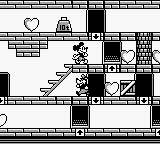
\includegraphics[width=.6\linewidth]{assets/assets/dmg-bb/dmg-bb-10.png}\par\pagetwodescription Here’s Roger, and Bugs, and Mickey, and Bugs again. Note that they all have very similar pixel height.
\vskip 6pt
\end{figure}
The Game Boy features a 160 by 144 pixels screen. Even by 1989 standards, this was low. Console games used CRT TVs, which featured an interlaced 480 or 576 vertical lines signal. I don’t want to get into the nitty-gritty complexities of interlaced signals, but I need to mention that a console like the NES pushed 256 by 240 pixel images (most TVs did not display the top or bottom~8 rows of pixels, which means you have visible 224 rows) and did not interlace another image. Consoles simply used the regular non-interlaced resolution of a TV. Even with these caveats, consoles had a much higher resolution than the Game Boy. This is not even talking of PC gaming, which had started using the VGA graphics standard and its roomy 640 by 480 pixels non-interlaced resolution in 1989.

\begin{figure}[hbt]
\vskip 10pt
\centering 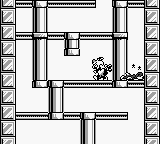
\includegraphics[width=4.85cm]{assets/assets/dmg-bb/dmg-bb-11.png}
\vskip 6pt
\end{figure}
When bringing the concept of \emph{Roger Rabbit} to the Game Boy, Kemco chose not to resize the characters, keeping them at the same pixel count. Every character used as many pixels as on NES. So here, with this underrated puzzle-action game, we have one of the most important decisions ever taken regarding Game Boy: characters should not get smaller, you just won’t see as much of the level around them. I’ve talked about this already in my \emph{Mega Man I} article but here we have the very first example of it. In a game based on environmental hazards like \emph{Mega Man}, it’s a tough nut to crack. With a simple concept like \emph{Crazy Castle}, where you’re on one vertical plane and you’re unable to jump, facing usually one enemy at a time, it made a lot of sense to keep Mickey and Bugs with the same level of detail as on a TV. The only thing you needed to be careful about was your level design;~make sure your levels reflect your limited view and you’re good. This simple decision will immediately become the standard for all future platformers on Game Boy.

\FloatBarrier\needspace{10mm}\section*{Easier on Game Boy? Not With Those Controls}\nopagebreak[4]

\begin{wrapfigure}{R}{0pt} 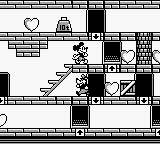
\includegraphics[width=.45\linewidth]{assets/assets/dmg-bb/dmg-bb-12.png}\end{wrapfigure}
\emph{The Bugs Bunny Crazy Castle} is not giving you a life bar or a second chance; you need to gather all eight carrots in each level in one attempt. If you die by touching any of the enemies on the map, you need to start that level again with zero collected carrots. So it’s one of those games that has lives where it makes no sense having them. There are passwords so you can always continue trying the same level, and you never reuse your progress within a level, you always start from zero. \textbf{So why does it have lives?} Because games back then had to have lives, that’s why.

One interesting feature is what the game calls \emph{video}. It’s a way to show you a replay of your last played level. There’s no mystery to how they did it; the game has zero randomness so just repeating your inputs can replay exactly what happened. It’s still impressive, even with this simple explanation.

Since the game is unforgiving, it should have generous controls to help you; instead they’re as unforgiving as the game. The second you go up a staircase you can’t cancel it. You actually move forward instead of staying still if you press up or down when not in front of stairs. This means that you could be trying to evade an enemy by going up steps but since you’re not in the exact spot to go up you instead rush headlong into that enemy.

The game has unforgiving mechanics and controls but it does not mean it’s hard. I skipped around using passwords and I thought it was suddenly going to be too hard to beat but levels stay surprisingly manageable. I even beat the last level, level~80, after five or six tries.

\FloatBarrier\needspace{10mm}\section*{Conclusion}\nopagebreak[4]

Making a dumbed down, licensed, easy version of a harsh 1983 game worked. \emph{The Bugs Bunny Crazy Castle} on Game Boy in 1990 ended up in the same position as \emph{Lode Runner} on Famicom in 1984. It was not particularly good but what else are you going to buy? It sold at least a million copies. It’s as if Kemco planned it that way. I bet they knew that it was better for them to release a simpler game early than a more complicated game later. They hit the ground running when everybody else was just getting started. Their next Game Boy release, \emph{The Sword of Hope}, would release in December of 1989 two months later and indeed be a more complicated RPG/Adventure game hybrid.

Play \emph{The Bugs Bunny Crazy Castle}; you’ll be able to see what \textbf{a lot} of people were playing early on in the Game Boy’s life. They had very few other choices until 1991. To them, and to us by extension, it’s essential.

\begin{figure}[hbt]
\vskip 10pt
\centering 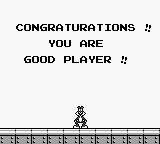
\includegraphics[width=4.85cm]{assets/assets/dmg-bb/dmg-bb-13.png}
\vskip 6pt
\end{figure}



\begingroup \chapter*{The Sword of Hope}\markboth{The Sword of Hope}{}\addcontentsline{toc}{chapter}{The Sword of Hope} \endgroup
\begin{figure}[H]
\vskip 4pt
\centering

\includegraphics[width=.75\linewidth]{assets/assets/dmg-se/dmg-se-1.jpg}\end{figure}
\begin{itemize} [nosep]




\item Japanese release in December 1989







\item North American release in June 1991







\item European release in 1991

















\item Developed by Kemco

\end{itemize}\noindent

\newpage\FloatBarrier\needspace{10mm}\section*{IAKESOCMEK}\nopagebreak[4]
\begin{wrapfigure}{L}{0pt} 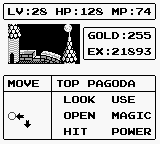
\includegraphics[width=.45\linewidth]{assets/assets/dmg-se/dmg-se-2.png}\end{wrapfigure}
I’m happy I experienced \emph{The Sword of Hope}, even if I could not find the energy to finish it. It’s really unique. It’s a game I knew next-to-nothing about and that I’m now fascinated by. \emph{The Sword of Hope} was made by Kemco who had just ported the MacVenture games to Famicom and NES. They had obviously intended to make a game in a similar vein but with a battle system lifted straight from \emph{Dragon Quest}. They did not hit a gold vein: it’s reasonable for an early title on Game Boy to be this experimental but peanut butter and jelly it ain’t. The mix of RPG and adventure game just fundamentally did not work. Looking at a game that tries its best but does not work is still valuable and essential.

\begin{figure}[hbt]
\vskip 10pt
\centering 
\includegraphics[width=.75\linewidth]{assets/assets/dmg-se/dmg-se-3.jpg}\par\pagetwodescription Like Nuts and Gum.
\vskip 6pt
\end{figure}

\FloatBarrier\needspace{10mm}\section*{Adventure Games Primer}\nopagebreak[4]

Back when \emph{The Sword of Hope} was released in Japan in 1989, adventure games had evolved into a very specific genre of video games but they were still at the core the evolution of text adventure games. Games like 1980’s \emph{Zork I} allowed you to wander and interact with a large world through text alone, and as computers became more powerful developers had the brilliant idea of replacing the descriptive text with images. A new genre, called adventure games, was born that used graphics but still allowed the frustrating experience of text input for any interaction:

\noindent{\codeintextfont > pick up sword\newline I DO NOT KNOW WHAT "up" IS\newline > pick sword\newline CANNOT "pick"\newline > take sword\newline YOU PICK UP THE SWORD. WHAT DO YOU DO NEXT?\newline > go to hell !!!\newline I DO NOT KNOW WHAT "to" IS\newline > }

Available on home computers, an expensive luxury at the time, with the best graphics out of any other game type, adventure games were using the limited PC technology to great effect. They also featured a newfangled thing that few other games had: a story. Compared to what is available today, this was laughable but do not dismiss the appeal of having a king give you your mission as you are playing the game. We take it for granted today but in the early ’80s having the story of the game unfolds as you are playing was a luxury reserved for the most dedicated video game players who could afford an expensive computer. NES players were stuck reading the manual to get a game’s story in the early days of the console.

By 1989, adventure games had moved away from text entry for every action and embraced menu-based interfaces. This was thanks in large part to Enix’s Yuji Horii. In 1984 he made \emph{Hokkaidou Rensa Satsujin: Ohotsuku ni Kiyu} for the NEC~PC-6001, a Japanese 8-bit computer. This was the sequel to his previous game, \emph{Portopia Renzoku Satsujin Jiken} which we usually know in the West as \emph{The Portopia Serial Murder Case}. Horii did not like the text parser of adventure games and so replaced it with a menu-based command system. It basically presented you with every verb in the parser from the get go, eliminating the guesswork of what words to use. His team was then tasked to port \emph{The Portopia Serial Murder Case} to the Famicom Disk System. They replaced the complex text entry of \emph{The Portopia Serial Murder Case} with the menu system of its computer sequel thus bringing the genre into the console space in very successful fashion. Westerners might dismiss the importance of this; don’t fall into that trap. We might have never gotten \emph{Hokkaidou}, \emph{Portopia} or the myriad adventure games that followed in their footstep on Famicom Disk System but this is because localizing them was never envisioned, not because those games are unimportant. Horii would use the lessons learned with \emph{Portopia} for his next project: the seminal role-playing game \emph{Dragon Quest}, a game of dizzying influence. With \emph{Dragon Quest}, he basically did the same thing he did with \emph{Portopia} again: he simplified the gameplay systems of a western genre, this time the role-playing game. Before \emph{Dragon Quest}, RPGs were usually a complicated, text-heavy affair. Think of a video game spreadsheet. Horii and his team got rid of anything that wasn’t absolutely necessary and made it easy for the player to understand what was happening. He also gave the player only a slight setback when they died; you only lose half of your money, and you’re brought back to the starting point of the game. This style of RPG referred to as the Japanese RPG or console RPG, is fundamentally the same to this day.

\begin{figure}[hbt]
\vskip 10pt
\centering 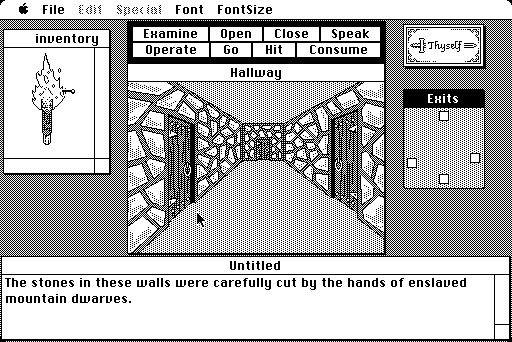
\includegraphics[width=.6\linewidth]{assets/assets/dmg-se/dmg-se-4.png}
\vskip 6pt
\end{figure}
Amongst these exciting times of new genres being born and iterated on, we have Kemco Sekai who was carving its own slice of the Famicom adventure genre by porting the so-called MacVenture games starting in 1988. Released by ICOM innovations on the Macintosh starting in 1985, \emph{Déjà Vu}, \emph{Uninvited} and \emph{Shadowgate} were some of the most innovative adventure games of their time. They used the Macintosh’s mouse, which meant you dragged the items in your inventory, clicked on your selected actions, and used a minimap to travel around: they were very forward-looking games with a lot of tactile feedback that took Yuji Horii’s innovation another step forward.

\begin{figure}[hbt]
\vskip 10pt
\centering 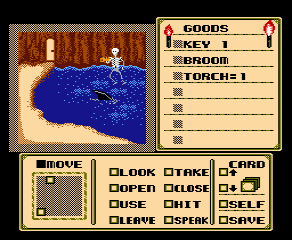
\includegraphics[width=.6\linewidth]{assets/assets/dmg-se/dmg-se-5.png}
\vskip 6pt
\end{figure}
They were also incredibly unfair, killing you for the slightest of mistakes. This is not a joke, if you forget to relight your torch in \emph{Shadowgate}, when it extinguishes, you’ll break your neck in the dark and die! It is obvious that \emph{The Sword of Hope} owes a great deal to the Kemco port of \emph{Shadowgate} on NES, the fantasy game in the series. It has the same minimap concept, the same vibe, and a very similar interface. It just has a Dragon Quest clone bolted on top of it.

\FloatBarrier\needspace{10mm}\section*{RPG Through and Through}\nopagebreak[4]

I’ve talked a lot about \emph{The Sword of Hope}’s adventure lineage but you really spend three quarters of the game playing an RPG, not an adventure game. Its adventure game lineage might be somewhat convoluted but its RPG roots are dead simple to understand; it’s just a copy of the first \emph{Dragon Quest}. I could go on and on about the spell list or the statistics but there’s nothing to say. They took \emph{Dragon Quest}, added more redundant spells and allowed you to fight more than one enemy at a time. Its close proximity to \emph{Dragon Quest} brings me to one of my pet peeves with the Game Boy library: I can’t find an original mainline RPG. I don’t mean that RPGs on the system are bad but they all have something eccentric about them. When I mean mainline, I’m thinking classic \emph{Final Fantasy}, \emph{Dragon Quest} or \emph{Final Fantasy IV} on SNES. Very R-P-G. High-fantasy setting, straightforward combat systems. On Game Boy, I can’t find anything original of that exact style. I’ve previously talked about the madness of \emph{The Final Fantasy Legend} (the sequels are just as crazy). \emph{Lufia} has procedural dungeons that kind of spoil the fun. \emph{Pokémon} is \emph{Pokémon}. You have the first three \emph{Dragon Quest} titles, but they’re not original Game Boy games. And \emph{Great Greed}, oh boy, let’s not even broach \emph{Great Greed}.

\begin{figure}[hbt]
\vskip 10pt
\centering 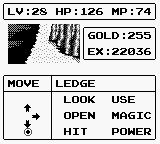
\includegraphics[width=4.85cm]{assets/assets/dmg-se/dmg-se-6.png}\par\pagetwodescription Does this look like the work of a team that finished the artwork?
\vskip 6pt
\end{figure}
I was surprised to find that there’s a normo RPG hiding underneath the adventure game veneer of~\emph{The Sword of Hope}. But there’s an adventure game veneer, so I’m still not satisfied in my desire for a mainline RPG on Game Boy; the search persists.

But the RPG that \emph{The Sword of Hope} offers is terribly boring. I guess that’s the problem with an RPG with so few choices to make; when your options are attacking or a spell that basically amounts to the same thing, without any variation in enemy type, battles have no meaning and turn into a numbers game. Can you get to where you need to go before you run out of HP, MP, and recovery items? If you grind long enough, you invariably always can. There’s no agency, you’re just pressing the A button until you’re bored. The question becomes whether you can suffer through all the grinding. As I’m getting older, the answer becomes no more often than not. I do not have the energy and time to waste on this. I can’t grind and grind and grind because someone in 1989 decided that was how an RPG worked. So I’ve decided halfway through the game to just punch in an end-of-game password and try my luck from there:

\begin{figure}[hbt]
\vskip 10pt
\centering 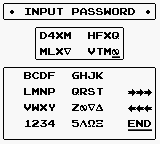
\includegraphics[width=4.85cm]{assets/assets/dmg-se/dmg-se-7.png}\par\pagetwodescription Salvation?
\vskip 6pt
\end{figure}

But it’s not very helpful; while you don’t have to worry about fights and you one-shot all the enemies, you still lose an inordinate amount of time in battles. Enemies are represented with dots on your minimap and if there’s a dot in the direction you want to go, you will have no choice but to fight a battle \textbf{instead of} moving. So you could be stuck for 5–6 battles on the same screen trying to go north. Had they simply changed it to forcing a battle \textbf{after} your move it would have made it completely fine. So even starting from a fully decked-out save and walking to the end boss, knowing what you need to do to get there is still an unbearable chore.

\begin{center}
\quad\vspace{4pt}\adjustbox{valign=t}{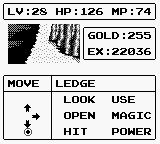
\includegraphics[width=.45\linewidth]{assets/assets/dmg-se/dmg-se-8.png}}
\quad\vspace{4pt}\adjustbox{valign=t}{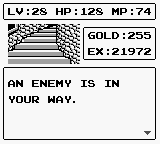
\includegraphics[width=.45\linewidth]{assets/assets/dmg-se/dmg-se-9.png}}
\end{center}

Which I guess teaches me (and you) a very important lesson about games: don’t stop the player from doing what they want to do. Punish the player if you must but putting a randomized roadblock in front of your audience only serves to disengage them. You lose any interest quickly when you try six times in a row to go south but you end up in a battle instead, however easy the battles are. Imagine the developers knew their battles were boring; could they have simply removed them and shipped an adventure game? No, the game would have been too simple. There’s no real puzzle in the game, nothing much to do except figuring out the routes and what thing to interact with. So the RPG elements are an essential part of the game, no matter how boring they are. I can imagine the developers knowing they didn’t have a champion on their hands but still pushing forward, knowing that this early in the life of the Game Boy, a subpar title could still be very successful. They had done exactly that a couple months before with \emph{Mickey Mouse/The Bugs Bunny Crazy Castle}.

\FloatBarrier\needspace{10mm}\section*{What?}\nopagebreak[4]

\begin{wrapfigure}{L}{0pt} 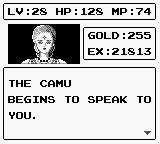
\includegraphics[width=.45\linewidth]{assets/assets/dmg-se/dmg-se-10.png}\end{wrapfigure}
To top off how boring the RPG part of the game is, the text is poorly translated from Japanese. I definitely believe that the translation was made by a non-native speaker. Sentence structures are weird, word choices are sometimes strange but this could all be explained by limited character space. The thing that confirms we have a second-language translator are the jokes. They’re obviously the work of someone with a limited grasp of how English humour functions. For once with the Game Boy Essentials project, I can say something as a true professional: I have a degree in Second Language Acquisition, specifically English. And this game is at the language level of one of my first year student trying their best. Definitely not on the level of a professional translator, even on their worst day.

\FloatBarrier\needspace{10mm}\section*{Conclusion}\nopagebreak[4]

Maybe someday in the future I’ll forget the brain-dead battles, revisit it and finish it. For the time being, I’m happy saying it is essential without saying you need to finish it. You just need to try it out a bit to understand its flaws and why they make it so boring to play for more than a couple of minutes.



\begingroup \chapter*{Mega Man II}\markboth{Mega Man II}{}\addcontentsline{toc}{chapter}{Mega Man II} \endgroup
\begin{figure}[H]
\vskip 4pt
\centering
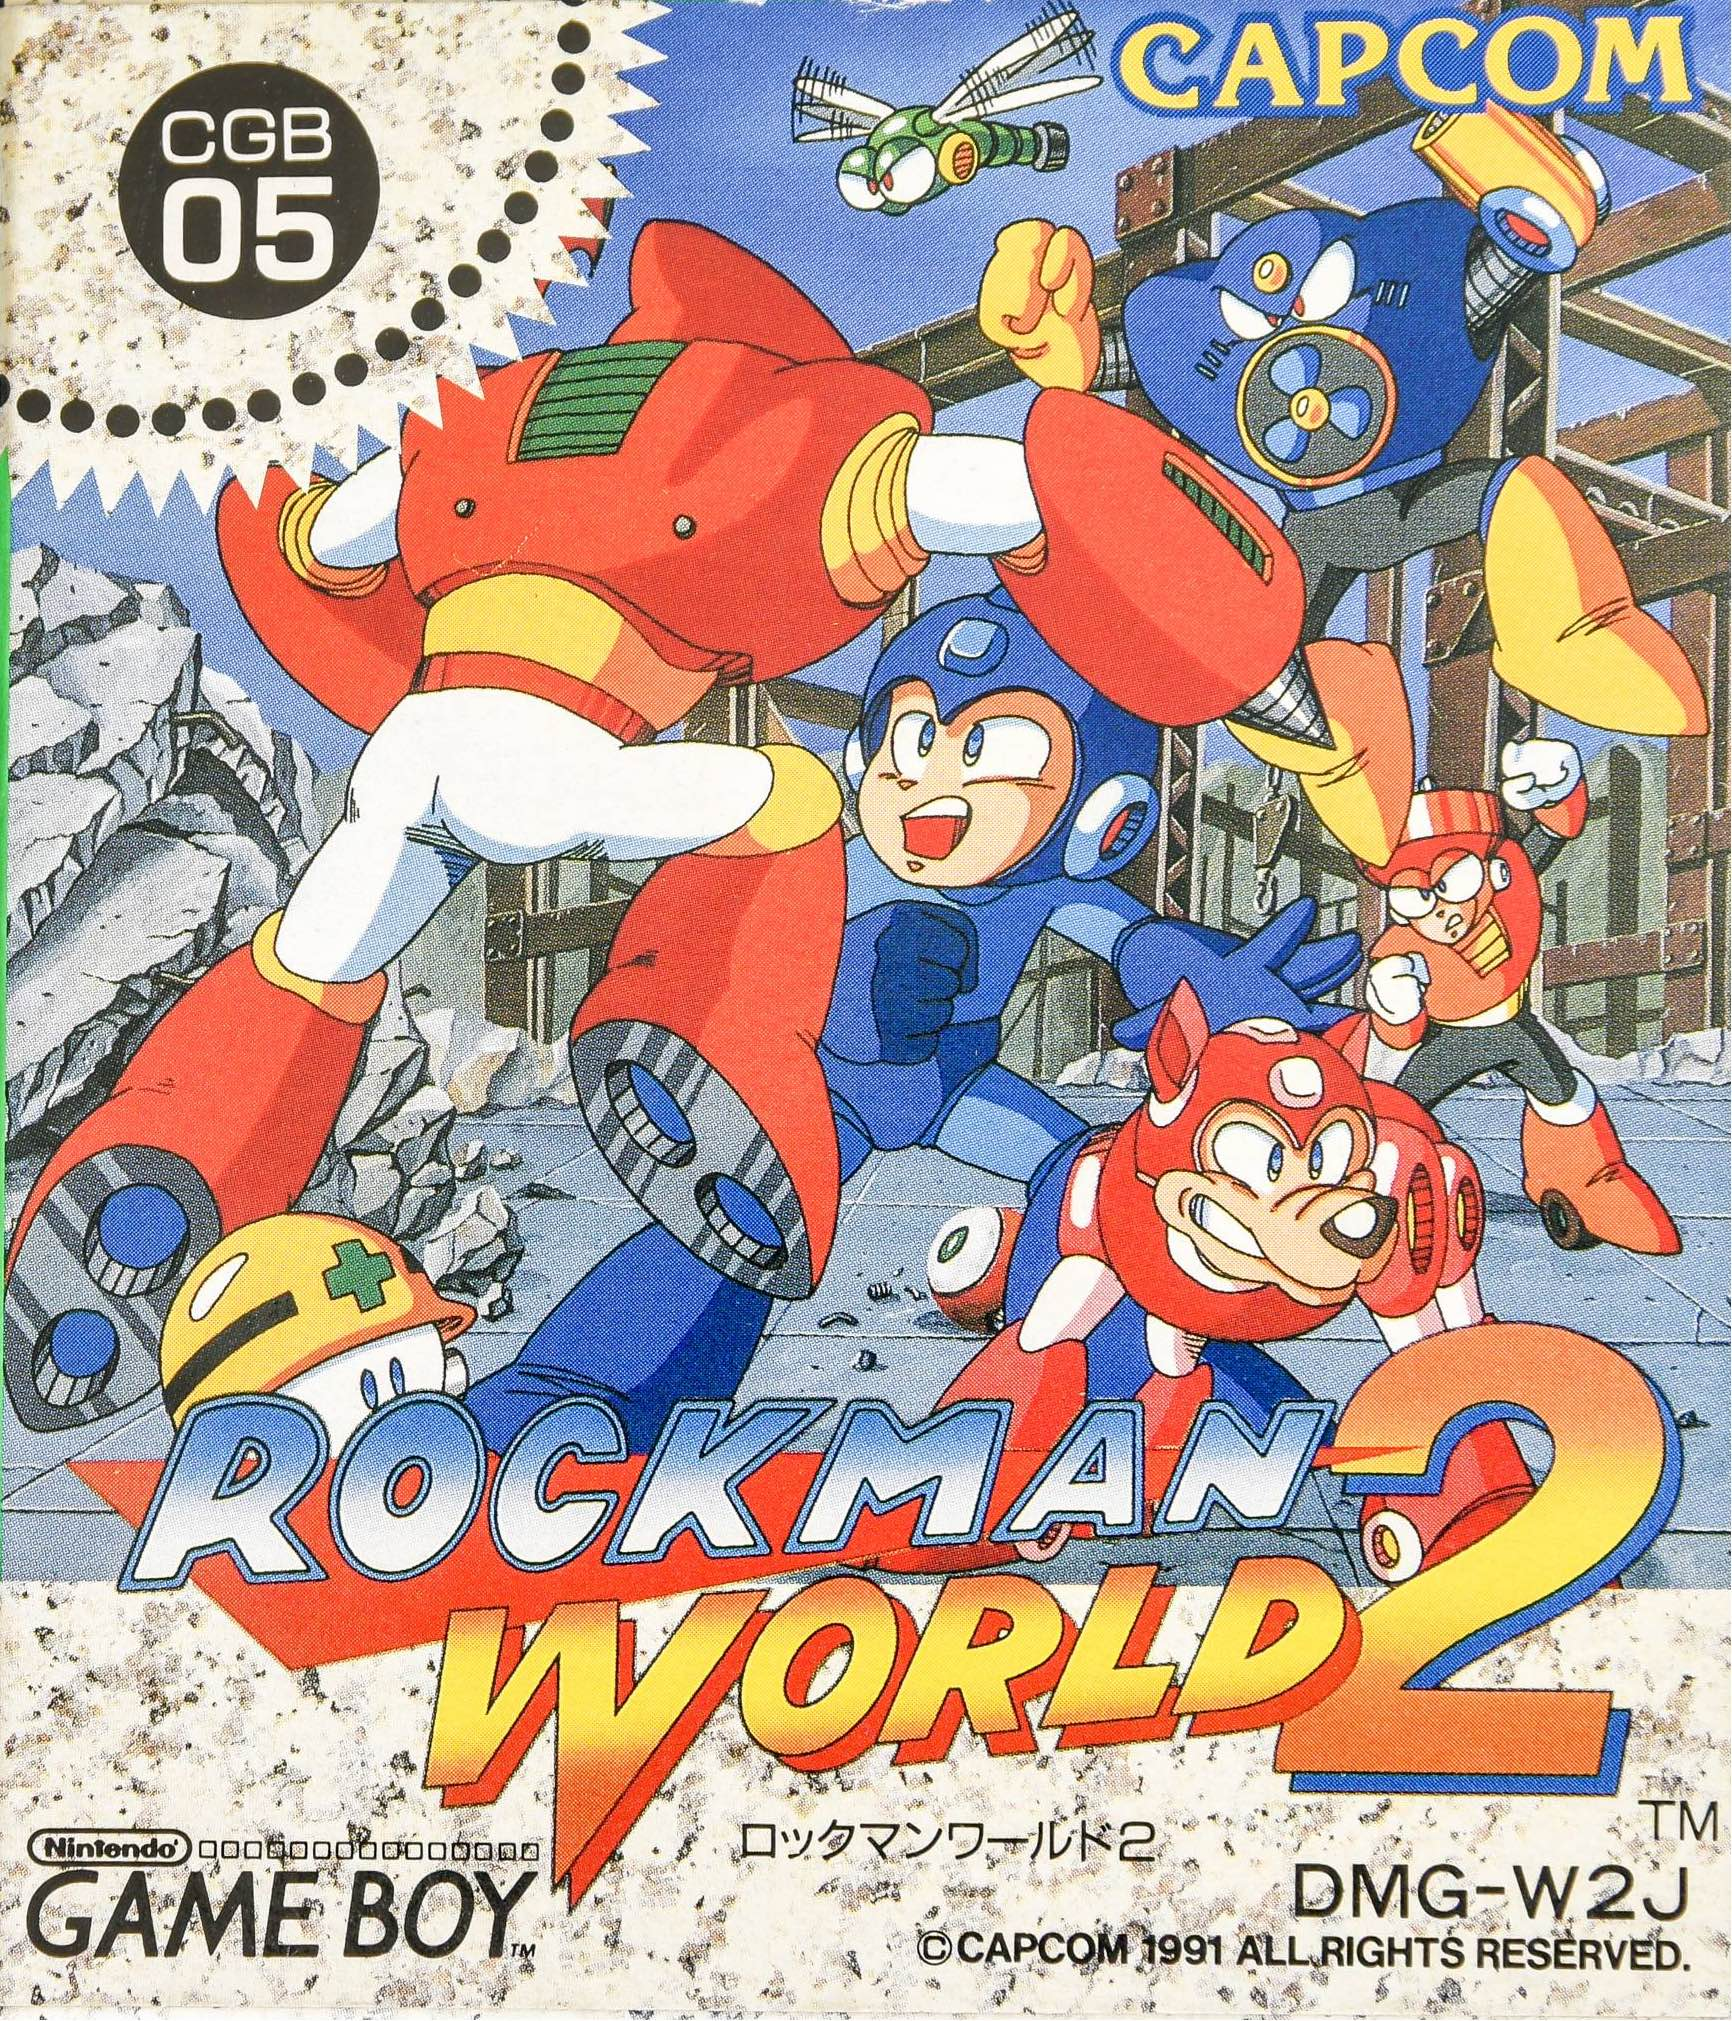
\includegraphics[width=.75\linewidth]{assets/assets/dmg-w2/dmg-w2-1.jpg}\end{figure}
\begin{itemize} [nosep]




\item Japanese release in December 1991







\item North American release in February 1992







\item European release in 1992







\item Australian release in 1992







\item Asian release in 1992







\item North American release in 1998
\begin{itemize} [nosep]\item Player’s Choice\end{itemize}\noindent






\item Japanese release in March 2001
































\item Developed by Biox

\end{itemize}\noindent

\newpage\FloatBarrier\needspace{10mm}\section*{Another Failed Attempt?}\nopagebreak[4]
\begin{wrapfigure}{L}{0pt} 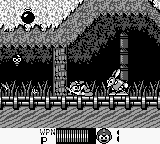
\includegraphics[width=.45\linewidth]{assets/assets/dmg-w2/dmg-w2-2.png}\end{wrapfigure}
The NES \emph{Mega Man} titles are not perfect; far from it. They’re great works of art though. Their controls are tight and responsive because of obvious perfectionism on the developer’s part, the level design is usually fun and inventive, the games are unfair but usually for the right reasons. Because of all this they’re a cultural standard that is used to judge sprite-based platformers to this day. They’re beloved, and they deserve it.

Comparisons between both families of games, NES and Game Boy, are inevitable. It’s absolutely fair; no one can look at an artistic project in a vacuum. And so the NES originals elevate the Game Boy games spun off from them by proxy. They make them better because when you play them, you’re obviously pushed into thinking of the NES games they are meant to echo. \textbf{This game on my Game Boy is just like the one on my TV!} While the first Game Boy game managed to carry out this task with limited success, managing to bring the concepts of \emph{Mega Man} to a screen with fewer pixels in an ultimately unfair game, the second title does the opposite. It’s too easy and too dumb to really ever make you feel like you’re playing a real \emph{Mega Man} game. That it was made by a small-time developer with very humble successes helps to explain this failure. Looking at what others have said about \emph{Mega Man~II} on Game Boy, people seem happy that you can finish this second title since it’s much easier than the first. I’d argue ease of play is not a very \emph{Mega Man} thing to do; you want inventive ways to punish you to make you sharp and swift. Ultimately, just like with the stilted \emph{Mega Man: Dr. Wily’s Revenge}, \emph{Mega Man~II} is essential because of its mistakes and problems. They’re just completely different.

\FloatBarrier\needspace{10mm}\section*{Note on Naming Conventions}\nopagebreak[4]

The NES and Game Boy \emph{Mega Man} games share the same titles which makes it confusing to differentiate between titles. They do, however, have a neat little quirk to help differentiate them: the NES titles use Arabic numbers (2,3,4) while the Game Boy titles use Roman numerals (III, IV, V). So I’ll use those to differentiate them. Keep in mind that in Japan the Game Boy series was called \emph{Rockman World}, which I might also write to be extra clear.

\FloatBarrier\needspace{10mm}\section*{Biox?}\nopagebreak[4]

Let’s start with two facts: One, \emph{Mega Man: Dr. Wily’s Revenge} was too hard for most people. Two, the next game, \emph{Mega Man~II} was released within the same year, was made by a different developer and is much easier. So what happened to cause this? Was Minakuchi sacked because they made a game that’s too hard? I implied as much in my article about the first game, but I’m not so sure anymore after thinking about it a bit more. I think Capcom wanted as many \emph{Mega Man} games released on Game Boy as quickly as possible and they devised the way to do it: adapt and remix the previous NES games using multiple developers to do it. Having played \emph{Mega Man~II} now, I think Biox never came back to do another game because their attempt was just not up to the task of being a fun adaptation of \emph{Mega Man~2}. So Minakuchi wasn’t sacked, Biox was.

Let’s start with the little details that Biox, the developer of \emph{Rockman World~2}, got wrong.

\begin{wrapfigure}{L}{0pt} 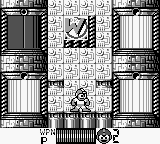
\includegraphics[width=.45\linewidth]{assets/assets/dmg-w2/dmg-w2-3.png}\end{wrapfigure}
First, when you hit a life pellet the game doesn’t pause and play the little jingle. The game continues \textbf{while} your life increases. It’s not much, to be sure, but it’s a small but essential part of the experience of playing a \emph{Mega Man} title. \emph{Wily’s Revenge} did not have that~quirk, properly pausing the game while your life increased, which means that Biox either did it without realizing their mistake or thought getting rid of a staple of the games would be an improvement. It is such a staple of the \emph{Mega Man} franchise to have you stop mid-air, while your life bar replenishes and you can relax for a split second, safe in the knowledge that you are getting the life bars you sorely needed for the challenges ahead.

Second, the doors to bosses don’t stop the screen from scrolling. When you walk towards them, the screen keeps moving and you can see the corridor beyond. It doesn’t happen with every Dr. Wily door, just some. It breaks the illusion and the expectations you are supposed to have regarding this upcoming boss battle.

\begin{wrapfigure}{R}{0pt} 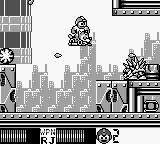
\includegraphics[width=.45\linewidth]{assets/assets/dmg-w2/dmg-w2-4.png}\end{wrapfigure}
Third, the weapon select menu sucks. \emph{Mega Man} weapon select menus have always kind of sucked; but here it sucks \textbf{and} they put the Rush Marine as the nearest selection. You use that maybe four times in the whole game, so you spend the whole game having to cursor past it for no good reason. GRRRR.

Fourth, the sound Mega Man makes when he touches the ground after jumping is high-pitched for no good reason. You just turn off the volume of your Game Boy after too long of this grating sound. The music also sounds like there’s always one note that’s off-key. Like the composer put in the wrong hex code every other note in each song just for kicks.

\begin{wrapfigure}{L}{0pt} 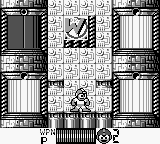
\includegraphics[width=.45\linewidth]{assets/assets/dmg-w2/dmg-w2-5.png}\end{wrapfigure}
Fifth, \emph{Mega Man: Dr. Wily’s Revenge} featured four bosses from \emph{Mega Man~2} in the boss rush before the final battle instead of having you repeat the same ones again. This was a welcome surprise, a hidden way to make the game meatier. Here for \emph{Rockman World~2}, Biox used the same surprise again but went one step further and included a full remixed \emph{Mega Man~3} level before each extra \emph{Mega Man~3} boss you have to face. I guess it’s nice but it’s clunky; half of the game starts from the boss rush room. Luckily they give you a password after you finish each new boss but it’s a grating little oversight.

\begin{wrapfigure}{R}{0pt} 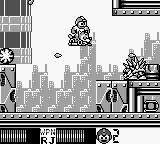
\includegraphics[width=.45\linewidth]{assets/assets/dmg-w2/dmg-w2-6.png}\end{wrapfigure}
Sixth, Rush Jet works for too long. Rush Jet is the power-up that allows you to call your robot dog as a flying sled you then ride in the air, allowing you to basically bypass any challenge you deem too hard. NES \emph{Mega Man} games knew they had to make Rush Jet useful but only for a short hop. Here it’s just too useful. It is so slowly sipping power that it’s totally overpowered turning any jumping section meaningless. You simply call Rush Jet and fly over everything that’s causing you any trouble.

To me, all those little details add up. The \emph{Mega Man} games on NES are extremely conservative. The improvements and changes to the core formula are very calculated. The dash, Rush the robot dog, the charge shot and the rest are all additions to shake up the underlying formula \textbf{which stayed the same for six games}. That the developers at Biox broke the underlying formula shows their lack of understanding of what is ultimately the appeal of Mega Man. The people at Minakuchi excelled at getting the fundamentals right, even though their game was just as flawed.

\FloatBarrier\needspace{10mm}\section*{Clocks?}\nopagebreak[4]

Here’s another example of how the people at Biox missed the appeal of \emph{Mega Man}. The Clash Man level on NES is very fun as an environment. You ascend a tower of tubes until you reach the top of the atmosphere to a dark sky devoid of stars. Then you reach the boss high up in space and fight him. Boom, that’s pure unadulterated \emph{Mega Man}. The Game Boy Clash Man level has you ascend at first until you reach a background of mountains. Then you start going down and the walls of the level are suddenly a different tileset. The concept of the NES level is completely abandoned. I feel like different people designed different sections of levels and they connected them together haphazardly. They didn’t think of creating an experience they just went ahead and made levels, making sure it wasn’t too hard. They didn’t make sure it was challenging or cohesive or fun or anything, the modus operandi was \textbf{not too hard}. This game was made quickly, and it shows! You end up with a disjointed experience that feels more influenced by a short development time than by the Mega Man series on NES. Time seems to be the theme of the game here, and there’s this whole back story with time travel. To hammer the point home, the last level of the game features clocks in the background, more specifically the clocks from Dali’s \emph{Persistence of Memory}. What?

\begin{figure}[hbt]
\vskip 10pt
\centering 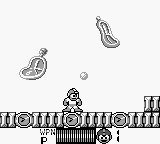
\includegraphics[width=4.85cm]{assets/assets/dmg-w2/dmg-w2-7.png}\par\pagetwodescription You’d usually find \emph{Mega Man} inspirations in anime, not modern art!
\vskip 6pt
\end{figure}

\FloatBarrier\needspace{10mm}\section*{My Biggest Problem}\nopagebreak[4]

The biggest battle of the game, the thing you should be most excited about is against a dude on a pogo stick!

A pogo stick!

\textbf{A pogo stick!}

And it’s not just any dude. It’s an evil, future Mega Man that Doctor Wily has somehow transported back in time to fight present day stick-in-the-mud Mega Man.

\textbf{Evil future Mega Man on a pogo stick!}

\textbf{A POGO STICK!}

How? How? \textbf{How?}

It is not a rhetorical question. I am dead serious. What confluence of madness, drugs, translation, laissez-faire and early 90s Japanese miracle bubble mentality led them down the path of future evil Mega Man on a pogo stick? The Mega Man series is not known for its serious attitude. You fight robot rabbits who throw robot carrots at you. Robot birds who throw eggs from which emerges a throng of mini robot chicks who lunge in your direction. I am talking here, to be clear, about robot baby birds guided missiles. How cool is that? There was, however, never anything so high-concept as evil future Mega Man on a pogo stick. The things you fight are cartoon robots based on animals, appliances, the general theme of the level’s boss. \emph{Mega Man: Dr. Wily’s Revenge} introduced the concept of a Mega Man Killer. It’s a robot built to destroy Mega Man that you fight on your way to Dr. Wily: the Darth Vader to the Emperor. In tropes term, a dragon.

So Biox ran with that idea and created a new dragon for their game. The best thing they could come up with was an idiot with sunglasses on his dumb stupid pogo stick.

Which, of course, this being a \emph{Mega Man} game, you then win as a weapon once you beat your future self. Mega Man steals his pogo stick from \textbf{himself}. It’s, of course, called Sakugarne and it is useless except against the last form of the last boss where it is secretly very strong. Of course.

I mean, they had to have come up with the character design before inventing a dumb pogo-based history for him, right? There’s no explanation anywhere in the game that he’s come from the future with his pogo stick.~.~. \textbf{OH MY GOD IS THE POGO STICK HIS TIME MACHINE?}

\begin{center}
\quad\vspace{4pt}\adjustbox{valign=t}{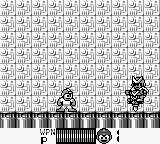
\includegraphics[width=.45\linewidth]{assets/assets/dmg-w2/dmg-w2-8.png}}
\quad\vspace{4pt}\adjustbox{valign=t}{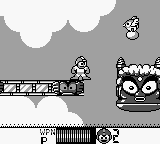
\includegraphics[width=.45\linewidth]{assets/assets/dmg-w2/dmg-w2-9.png}}
\quad\vspace{4pt}\adjustbox{valign=t}{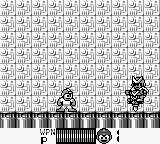
\includegraphics[width=.45\linewidth]{assets/assets/dmg-w2/dmg-w2-10.png}}
\end{center}

\FloatBarrier\needspace{10mm}\section*{Conclusion}\nopagebreak[4]

\begin{wrapfigure}{L}{0pt} 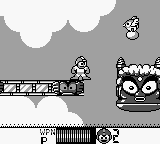
\includegraphics[width=.45\linewidth]{assets/assets/dmg-w2/dmg-w2-11.png}\end{wrapfigure}
My main problem with \emph{Mega Man~II} is that it’s an OK Game Boy game but it is not particularly worthy of the \emph{Mega Man} title. However, its flaws did not stop people from enjoying it; it was easier and still somewhat competent and it sold at least a million copies. Being after the most beloved NES title must have helped. It was quickly rereleased as a Players’ Choice title in 1993.

\emph{Mega Man} on NES is a reliable series. You’re always doing something invigorating throughout every game. You can count on it. On Game Boy, the series was definitely not reliable. After experiencing the first and second Game Boy cartridges in depth, I’ve seen too many ups and downs. That those two titles were made by different developers helps explain it: Biox could obviously not build on the knowledge learned by the developers at Minakuchi Engineering to make a better sequel. With that in mind, I’m looking forward to the return of Minakuchi with \emph{Mega Man~III}. I’ve played \emph{Mega Man IV} extensively and I love it so I can’t wait to play the third game; I have no idea whether it’s excellent like \emph{IV} or kind-of-bad like \emph{II}.

\begin{figure}[hbt]
\vskip 10pt
\centering 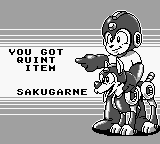
\includegraphics[width=4.85cm]{assets/assets/dmg-w2/dmg-w2-12.png}\par\pagetwodescription Oh go to hell with your goddamn pogo stick.
\vskip 6pt
\end{figure}



\begingroup \chapter*{Operation C}\markboth{Operation C}{}\addcontentsline{toc}{chapter}{Operation C} \endgroup
\begin{figure}[H]
\vskip 4pt
\centering
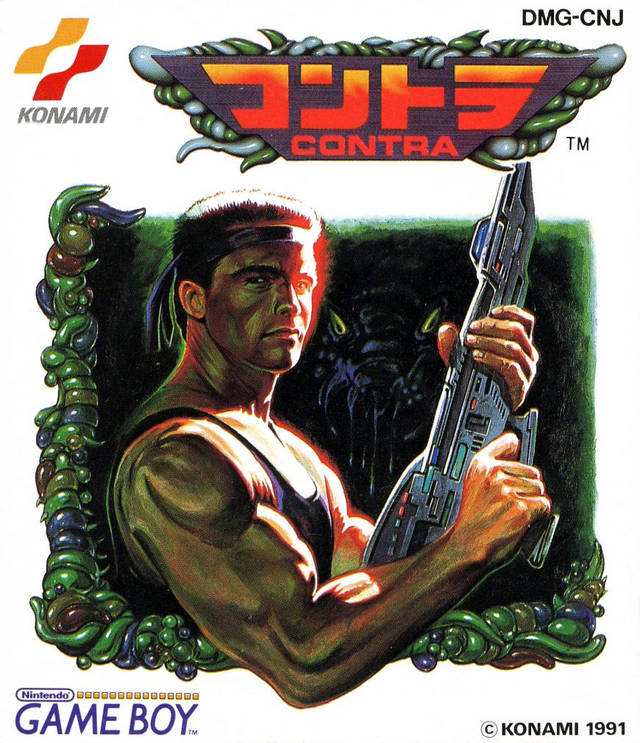
\includegraphics[width=.75\linewidth]{assets/assets/dmg-cn/dmg-cn-1.jpg}\end{figure}
\begin{itemize} [nosep]




\item Japanese release in January 1991







\item North American release in February 1991







\item European release in May 1992












\item Developed by Konami

\end{itemize}\noindent

\newpage\FloatBarrier\needspace{10mm}\section*{Baby Contra}\nopagebreak[4]
\begin{wrapfigure}{L}{0pt} 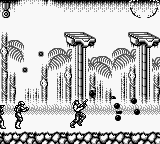
\includegraphics[width=.45\linewidth]{assets/assets/dmg-cn/dmg-cn-2.png}\end{wrapfigure}
Making a competent adaptation for Game Boy is not an exact science. In my previous article, I argued that Biox’s \emph{Mega Man~II} has the basic concepts done properly, but that they just mangled the execution. The skeleton is OK but the rest of the body is too weird.

On the other hand, Konami’s \emph{Operation C}, known in Japan as simply \emph{Contra} and in Europe as \emph{Probotector}, is the real deal. The sprite size, walking and jumping speed, level of detail, everything is well tuned, so the skeleton of the game is great. Then they went ahead and added all the trimmings. Levels, weapon selection, game length, enemy types, difficulty. All those details fit perfectly too. Konami really got it right, just like with their previous game I covered, \emph{Nemesis}. Once again, the fine people at Konami made an essential game. I still remember to this day the joy of playing this game when I was a kid. And I played this game late, since a friend first lent it to me around 1998.

\FloatBarrier\needspace{10mm}\section*{Collect S to Win}\nopagebreak[4]

\begin{wrapfigure}{R}{0pt} 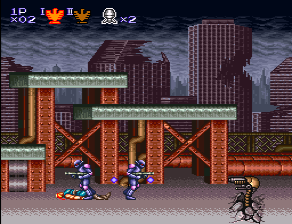
\includegraphics[width=.4\linewidth]{assets/assets/dmg-cn/dmg-cn-3.png}\end{wrapfigure}
Close your eyes and think of the \emph{Contra} games. What images come to mind? For me, it’s mostly \emph{Contra~III: The Alien Wars} on SNES and its hyperactive attitude. I think of explosions, frenetic jumping from missile to missile while flying through the air, and more explosions. That’s the later \emph{Contra} series’ attitude, having evolved its own style based on explosions and insane situations. But \emph{Operation C} came out earlier, when the games were action-packed to be sure but they were a bit more sedate. Their marketing and situations were clearly trying to bank on the love of \emph{Predator}, \emph{Alien} and \emph{Rambo} with a good measure of \emph{Commando} thrown in. I’m being nice here, they weren’t just going for the style of those movies, they were literally tracing promotional pictures for those movies to put on the game covers.

\begin{figure}[hbt]
\vskip 10pt
\centering 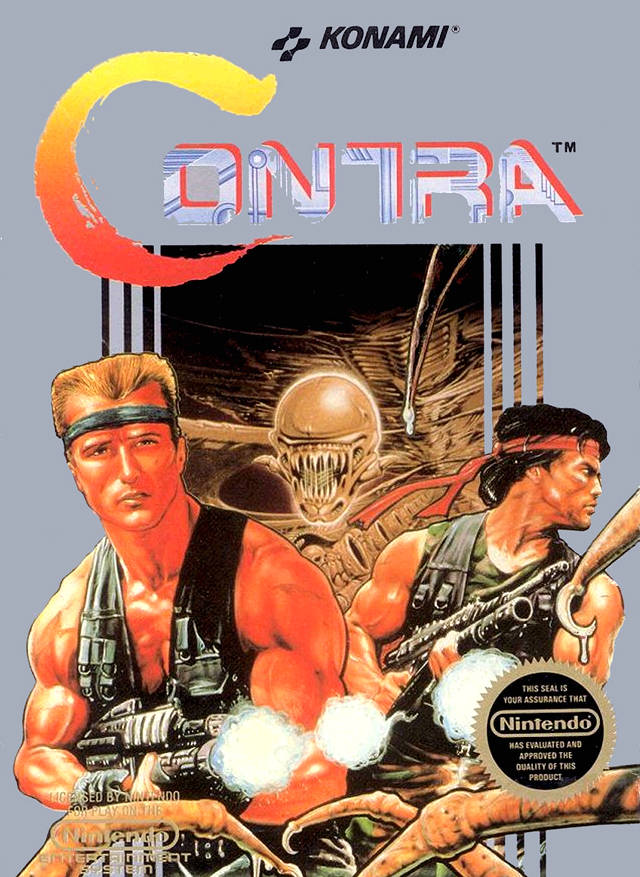
\includegraphics[width=.75\linewidth]{assets/assets/dmg-cn/dmg-cn-4.jpg}\par\pagetwodescription It’s Rambo and Matrix fighting against the Xenomorph! No wonder everybody \textbf{loved} Contra.
\vskip 6pt
\end{figure}

\begin{wrapfigure}{L}{0pt} 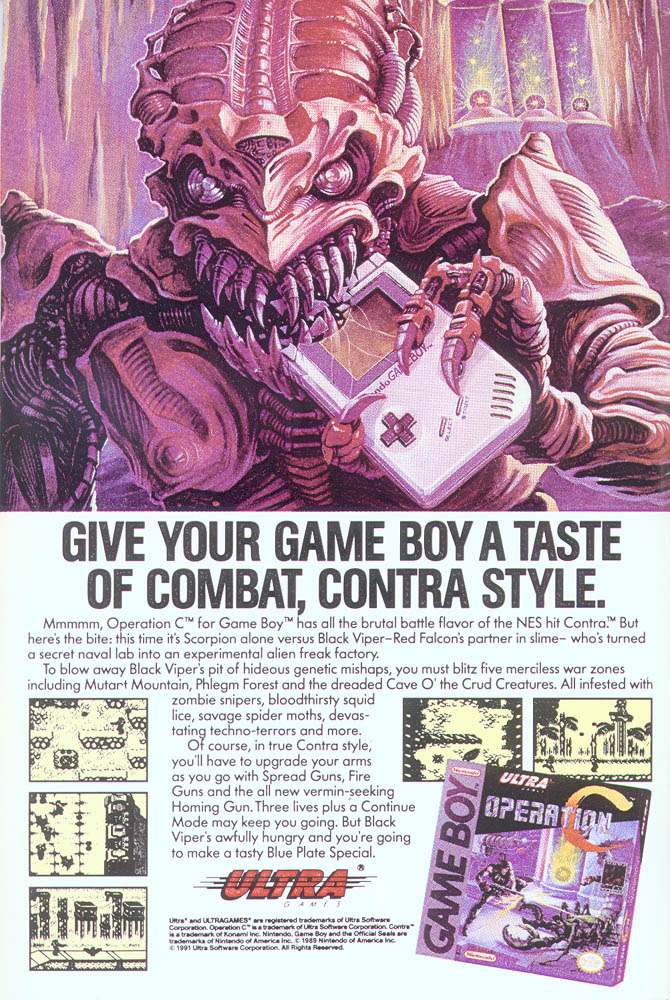
\includegraphics[width=.4\linewidth]{assets/assets/dmg-cn/dmg-cn-5.jpg}\end{wrapfigure}
Within those traced packages where games that were a bit more .~.~. subdued than what would suddenly burst through with 1992’s \emph{Contra~III}. What we have with \emph{Operation C} is the last hurrah of that classic \emph{Contra} era. The Japanese cover has a blatant mix of Michael Biehn and Arnold on its cover but the American game’s box is clearly not trying to sell us on a Stallone/Schwarzenegger video game, it’s forging a new unique identity for \emph{Contra} (fun fact: the artist for this cover, Tom DuBois, is now a hardcore Christian artist). The game itself is a Game Boy adaptation of the NES adaptation of the arcade \emph{Super Contra}. These three-step adaptations are way more common in video games than you might think and here we have one of my favourite ones. This little game is just awesome.

I often hear commentators, youtubers, podcasters start talking about a Game Boy game with: \emph{Even though it’s on Game Boy, it’s still good. How surprising!} These are benign comments not given much thought, a reflex to think that portable systems are somehow a lesser thing, that somehow the natural state of a portable game is to be bad. But there is no surprise that \emph{Operation C} is an extraordinary game. It was made by a company with a stellar reputation for quality in 1991, a small group of four internal developers used to the Game Boy. \textbf{Of course it’s good even though it’s on Game Boy!}

\begin{figure}[hbt]
\vskip 10pt
\centering 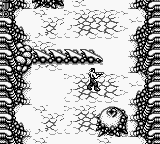
\includegraphics[width=4.85cm]{assets/assets/dmg-cn/dmg-cn-6.png}\par\pagetwodescription The Japanese version allows you to select any of the first four levels.
\vskip 6pt
\end{figure}

\FloatBarrier\needspace{10mm}\section*{Remember, Sully, When I Promised to Kill You Last?}\nopagebreak[4]

Let’s talk about the story. Actually let’s not because \textbf{I don’t care!} When I go on websites online to read about \emph{Contra} games there’s always this undue attention paid to the story and the timeline and how the American games are not set in the same period as the Japanese ones. It’s all useless hogwash! Nobody has ever played a \emph{Contra} game to continue exploring the rich story of the \emph{Contra} universe. You just want to walk right and kill stuff from 80s movies!

\begin{figure}[hbt]
\vskip 10pt
\centering \includegraphics[width=.75\linewidth]{assets/assets/dmg-cn/dmg-cn-7.jpg}\par\pagetwodescription The ad copy is clear that it only has single-player. It was important to warn people it did not have \emph{Contra}’s greatest feature: simultaneous coop.
\vskip 6pt
\end{figure}

\FloatBarrier\needspace{10mm}\section*{I Lied.}\nopagebreak[4]

The game is one Megabit (not byte), so it’s a very small program. This does not mean anything without context, so let’s bring it to something you will understand. \emph{Operation C} is twice as big as \emph{Super Mario Land} in size. That’s not big! \emph{Super Mario Land} is minuscule, with its small levels and very limited tileset. So \emph{Operation C} has more room in the cartridge for enemy types, for longer levels and more detailed tiles, but twice the size is not a panacea. We’re still talking about 131 kilobytes (not bits), a laughably small amount of space for a complete program with music and graphics. A small programmable space like that means the programmers and designers could not do everything they wanted. They could not draw and program too many enemies, meaning they had to reuse enemy types and their projectiles. They could not draw too many tiles, meaning the levels could not be too detailed. They had to get wise with the tiles they could fit on the cart to make interesting environments. Those are big limits to what you can do.

As the \emph{Contra} series got older, you had more and more unique situations that you faced that correlated directly with an increase in cartridge size. With \emph{Contra: Hard Corps} on Genesis, the series reached the apex of this evolution with a constant boss rush, with barely any reused enemy or environment to be seen. \emph{Contra} went from an intelligent repetition of enemies and patterns to a series of custom-built set pieces.

\begin{wrapfigure}{L}{0pt} \includegraphics[width=.45\linewidth]{assets/assets/dmg-cn/dmg-cn-8.png}\end{wrapfigure}
And \emph{Operation C} is the most repetitive of the \emph{Contra} games. The fourth level, one of the game’s two overhead level, has only two enemy types and one environmental hazard. Yet it manages to stay frantic and surprising. Even the boss reuses the same projectile as one of the enemy types in the level but its new projectile patterns make it fresh. They really stretched every little concept they built. It’s really surprising to see how much of the game is recycled while staying surprising and vibrant. They pull every trick in the book to make you forget the recycling.

Again in level four, you have those weird invincible protrusions that come out of walls to try and hit you. They use every permutation of pattern I can think of to give you a different challenge every time you encounter them, \textbf{and} they place enemies in varying places to make it more complicated to navigate around them. I urge you to play the game and look for the tricks the developers used to maximize their assets. It’s fun!

\FloatBarrier\needspace{10mm}\section*{The Size of Scene Elements}\nopagebreak[4]

The developers have applied the same lesson here as in \emph{Nemesis}. Everything in the game is a bit smaller than on NES, but not too small. You still don’t see as high or as far. They’ve made your character literally a head smaller.

\begin{figure}[hbt]
\vskip 10pt
\centering \includegraphics[width=.6\linewidth]{assets/assets/dmg-cn/dmg-cn-9.png}\par\pagetwodescription Literally a head smaller.
\vskip 6pt
\end{figure}

So your character is smaller but he’s not small enough to take the same amount of space as on a TV; he’s still so big that he eats up more space. That’s fine, as we’ve seen with \emph{Nemesis} and \emph{The Bugs Bunny Crazy Castle}. You adapt the gameplay to fit the screen resolution, and that’s what they did here. They were helped in this by how the series works. You see, the Contra dude (I steadfastly refuse to remember his name) is slower to move than Mega Man or most other characters in platform games. He’s not zipping around as fast and jumping as much. You move slower, have fewer jumps to clear and spend much more time aiming at enemies coming from all directions. Those concepts were much more suited to the smaller resolution of the Game Boy. You don’t need to redesign everything around your main character to make the game work; you just have to be looser with enemy aggressiveness and placement. They also limited the amount of flying enemies you see and kept the two overhead levels on a tight leash in terms of bullet hell. That makes \emph{Operation C} easier than the console or arcade versions because you can’t have enemies pop out on the screen at the same rate as on those; the screen is smaller and you’d be swamped. So enemies telegraph their moves a bit more, move a bit slower, shoot a bit less bullets. No enemies in \emph{Operation C} are as fast as the dogs in the first level of \emph{Contra~III}.

\begin{figure}[hbt]
\vskip 10pt
\centering \includegraphics[width=4.85cm]{assets/assets/dmg-cn/dmg-cn-10.png}
\vskip 6pt
\end{figure}

\FloatBarrier\needspace{10mm}\section*{Small Quality-of-Life Improvements}\nopagebreak[4]

The game introduces auto-fire to the series, meaning you can hold the A button to keep firing. That way you don’t have to mash the A button all the damn time. It’s a different approach that changes the game a lot, reducing the amount of time you spend aiming and it turns you into a firehose of bullets. You need to be challenged in different, less interesting ways because of that. It was a necessary change in hindsight to keep the series approachable and save our thumbs.

\begin{wrapfigure}{R}{0pt} \includegraphics[width=.45\linewidth]{assets/assets/dmg-cn/dmg-cn-11.png}\end{wrapfigure}
All subsequent games would use the same system, with \emph{Contra~4} having the genius idea of allowing both shooting methods. In \emph{Contra~4}, made by the fine folks of WayForward Technologies, holding the button gives you a satisfying, steady stream of bullets but mashing the button makes even more bullets appear, giving you that small edge you so often need. So you can rest your thumb on the button most of the time and mash when you get in a tight spot. It’s so intelligent as to be maddening. Why did nobody else thought about it before? Oh WayForward, how I like thee!

Don’t worry, I haven’t forgotten to talk about the Konami code too. On the North American (\emph{Operation C}) and European (\emph{Probotector}) releases, punching in the code allows you to access the level select from the original Japanese version. The Japanese (\emph{Contra}) version instead uses it to give you nine lives. Look up the GameFAQs description of what each code does for more details.

\FloatBarrier\needspace{10mm}\section*{Let Off Some Steam, Bennett.}\nopagebreak[4]

We need to talk about censorship, kids. First off, it’s not what you think. If a country has a legally binding review board that deems cultural content inappropriate for \emph{minors} and thus enforces that the material only be sold to adults, that’s not exactly censorship. Nobody’s harshly censored, you’re just deemed inappropriate for \textbf{sale} to children. An adult will have to make the call on whether or not their children can play those games.

\begin{center}
\quad\vspace{4pt}\adjustbox{valign=t}{\includegraphics[width=.45\linewidth]{assets/assets/dmg-cn/dmg-cn-12.jpg}}
\quad\vspace{4pt}\adjustbox{valign=t}{\includegraphics[width=.45\linewidth]{assets/assets/dmg-cn/dmg-cn-13.jpg}}
\quad\vspace{4pt}\adjustbox{valign=t}{\includegraphics[width=.45\linewidth]{assets/assets/dmg-cn/dmg-cn-14.jpg}}
\end{center}

So if a company then looks at its video game, thinks there might be \emph{a chance} its clear pastiche of all the movies glorifying war in the ’80s might be deemed inappropriate for children and then \textbf{voluntarily modifies its game to make sure its product can be sold directly to children}, that’s again not exactly censorship. So why am I talking about this? Because \emph{Contra} has a complicated history with European classification boards, that’s why. When the time came to bring the original \emph{Contra} arcade game to Europe, I guess the political heat on the Iran-Contra affair meant the name was deemed inappropriate: the arcade game was called \emph{Gryzor} in Europe. The sequel \emph{Super Contra} did not change its title in Europe, probably because by 1988 the whole political catastrophe was no longer in the news. Still, the series, ostensibly about shooting aliens and robots in the face, has forever been attached with the illegal smuggling of cash from secret Iranian arms deals to fund a brutal antigovernment rebel group in Nicaragua by the United States. And Konami did not innocently fall into this controversy. \emph{Contra} and \emph{Super Contra} start with jungle levels, which, of course, forces you to connect the game with the Contras themselves, and the original arcade title has a music track called Sandinista, after the socialist government the Contras were fighting against! So the people at Konami knew what they were doing. Even in North America they somewhat retired the \emph{Contra} name for a while, using \emph{Super C} and \emph{Operation C} to obfuscate the connection.

\begin{wrapfigure}{L}{0pt} \includegraphics[width=.45\linewidth]{assets/assets/dmg-cn/dmg-cn-15.png}\end{wrapfigure}
Now that’s just the entrée in the long history of \emph{Contra} and controversy; with the \textbf{console} version of \emph{Contra} in Europe, the German Protection of Young Persons Act reared its head. It’s a law meant to protect children and teenagers from being exposed to material deemed inappropriate for them. While most countries are content with having industry-regulated classification boards giving ratings to games, the German went one step ahead and made it a government-controlled board. Couple that with the fact that it is very clear that \emph{media carrying content glorifying war} is not to be sold to minors, and you have a skittish Konami. Let’s be honest here: \emph{Contra} is totally glorifying war. So Konami did the sensible corporate thing; they completely reskinned \emph{Contra} with robots instead of humans and changed the name for good measure to \emph{Probotector}. They then released this version for all of Europe. They self-censored.

\begin{wrapfigure}{L}{0pt} \includegraphics[width=.45\linewidth]{assets/assets/dmg-cn/dmg-cn-16.png}\end{wrapfigure}
They did this \textbf{of their own volition}, since they seemed to have never submitted \emph{Contra} in its original form for any classification in Europe. They only submitted the modified robot version. So every subsequent game, including \emph{Operation C}, replaced all the humans with robots. I kind of like it, the robots look rad. It’s a nice change of pace. I don’t think Europeans missed out on anything by having robot-on-robot action.

\FloatBarrier\needspace{10mm}\section*{Standard Collection Reissue}\nopagebreak[4]

\begin{center}
\quad\vspace{4pt}\adjustbox{valign=t}{\includegraphics[width=.45\linewidth]{assets/assets/dmg-cn/dmg-cn-17.png}}
\quad\vspace{4pt}\adjustbox{valign=t}{\includegraphics[width=.45\linewidth]{assets/assets/dmg-cn/dmg-cn-18.png}}
\end{center}
Just like \emph{Nemesis} and most of the early Konami Game Boy titles, it was rereleased with the four-volume \emph{Konami GB Collection} in 1997 in Japan and in 2000 in the UK. The same comments I gave to \emph{Nemesis} apply for \emph{Operation C}. The colour palette of the UK GBC version is woefully inappropriate, really giving credence to all the negative comments you get about the Game Boy Color’s pastel colours. You can often see the jagged edges where the tiles change colour palettes; it’s not a good job. What is interesting is that the European release keeps the unique title for the European market, \emph{Probotector}, but skips the replacement of the characters with robots. With the arrival of the current German classification board in 1994, what is and isn’t fair to release to minors in Germany had obviously changed. Oh and the \emph{Konami GB Collection} was never released in Germany anyway, just in the UK. All of this makes it the last game to use the \emph{Probotector} title (on consoles, Konami had stopped renaming their European versions after \emph{Contra: Hard Corps} on Genesis in 1994). They clearly just took the easy way out: the game still uses the Japanese version, since it features the level select absent from the North American and European original releases.

\FloatBarrier\needspace{10mm}\section*{Conclusion}\nopagebreak[4]

\begin{wrapfigure}{R}{0pt} \includegraphics[width=.45\linewidth]{assets/assets/dmg-cn/dmg-cn-19.png}\end{wrapfigure}
\emph{Operation C} is an essential step in the Game Boy story of Konami. It again shows that \emph{Nemesis} was not a fluke. The fine people at Konami seem to have understood the Game Boy right away. I have not talked so far about all of Konami’s output on Game Boy in the early days, with games like \emph{Motocross Maniacs}, \emph{Twin Bee}, the first \emph{TMNT} game and particularly \emph{Castlevania: The Adventure} showing other attempts by Konami that were not always successful. I’ll get to those in due time but I can say with confidence that Konami had a very good at-bat on Game Boy.

Compared with their compadres at Capcom who stumbled twice with their mascot Mega Man and the subcontractors they entrusted him with, Konami was on point from the get go on Game Boy by doing the job themselves.

\begin{figure}[hbt]
\vskip 10pt
\centering \includegraphics[width=.5\linewidth]{assets/assets/dmg-cn/dmg-cn-20.jpg}
\vskip 6pt
\end{figure}



\begingroup \chapter*{Mario’s Picross}\markboth{Mario’s Picross}{}\addcontentsline{toc}{chapter}{Mario’s Picross} \endgroup
\begin{figure}[H]
\vskip 4pt
\centering
\includegraphics[width=.75\linewidth]{assets/assets/dmg-apce/dmg-apce-1.jpg}\end{figure}
\begin{itemize} [nosep]




\item Japanese release in March 1995







\item North American release in March 1995







\item European release in July 1995







\item Australian release in 1995







\item Japanese release in March 2000
































\item Developed by Jupiter Corporation

\end{itemize}\noindent

\newpage\FloatBarrier\needspace{10mm}\section*{Nono}\nopagebreak[4]
\begin{wrapfigure}{L}{0pt} \includegraphics[width=.45\linewidth]{assets/assets/dmg-apce/dmg-apce-2.png}\end{wrapfigure}
I have a list of Game Boy games I want to check out and feature on Game Boy Essentials. With over 2000 titles released across the original Game Boy and Game Boy Color, I have looked at multiple sources to winnow the list into a reasonable amount of games to research further. I have yet to fire up every single game in an emulator, so I rely on a lot of common sense to figure out what is potentially essential. Initially, \emph{Mario’s Picross} flew under the radar for most people, me included. I came upon it by chance, only knowing \emph{Mario’s Picross} as an adaptation of nonograms by Nintendo. It was popular in Japan but nobody cared in North America, so Jupiter promptly stopped bringing their Picross games here. So knowing only this I decided to play the game for a minute and I fell in love. I went through the tutorial to learn the rules and liked it so much I immediately bought a book to try nonograms on paper. That’s how essential this game is; it will make you buy books!

\FloatBarrier\needspace{10mm}\section*{A Primer on Nonograms}\nopagebreak[4]

So what are nonograms anyway? A nonogram is a grid with numbers on its side indicating how many squares need to be pencilled in on each row and column. You apply logic to figure out which ones can be safely filled in and which ones can be safely discarded. When you’re done, you have a picture of an umbrella or a race car or something. To me nonograms are particularly soothing; you’re painting with logic instead of artistry, and I am way better at logic than artistry! It’s not that dissimilar to a Sudoku, but I’d argue it’s a more varied experience. It’s got more legs to get you to play just. One. More. Grid.

\FloatBarrier\needspace{10mm}\section*{It’s-a-Me, Market Buster!}\nopagebreak[4]

The question that fascinates me with nonograms is: why are they so utterly unpopular? Sudoku is everywhere, tends to be well-known, is the golden standard of \emph{book you buy at the cash register next to an Archie omnibus}. Why aren’t nonograms, which are ostensibly the same thing as Sudoku (fidgeting around with numbers and squares) not more popular? I’ve thought about it and I think it comes down to two things. First of, Picross is one of those rare paper game that’s better on a computer.

On paper, Picross is ostensibly about not making mistakes. If you make a mistake, it can easily propagate all over your nonogram like a virus and you’ve lost all your effort, since what you do has an impact on everything around it. So a one square mistake can propagate for dozens of squares before you realize you’ve messed up. So it’s a game about focus, about making sure your work is perfect at all times. When you screw up a nonogram on paper, you might as well throw the whole thing in the trash. It is stupidly difficult to figure out your mistake and walk it back. \emph{Mario’s Picross}, on the other hand, will always tell you when you make a mistake, completely changing the focus of the game from perfection to quick execution. You see, if the developers only warned you of mistakes without any consequence the game would be meaningless, you could just bash at random until you had found all the black squares. But the developers at Jupiter put a timer on every puzzle. And when you make a mistake, you lose time. Only two minutes at first, but you lose four and then eight minutes per mistake. When you have thirty minutes to complete the puzzle that means you could quickly lose all your progress. Then you’re thrown back at the puzzle select screen and you can start the same puzzle over from scratch, with a leg-up because you remember what you already did, but now you have to do it all over again. So \emph{Mario’s Picross} is a game about being as perfect as possible and properly \textbf{managing} your mistakes. I’d argue this is a more fun proposition than keeping perfect focus on paper.

Even though they are more fun as a video game, why are they absent from the books you buy at the grocery store? Beats me. I will obsess to an unreasonable degree about Game Boy games and their business prospects but I’m not going to start obsessing about the grocery store puzzle market. I’m not \textbf{that} much of a nerd.

The second reason I think nonograms are so unpopular is Nintendo will support something so well they steal all the oxygen from a genre. Since the Jupiter implementation of nonograms is more fun than doing it on paper, I don’t think anybody really saw the appeal beyond what Jupiter was offering. This would not be the first time they would do this to a genre. Look at the \emph{Mario Kart} or \emph{Legend of Zelda} franchises; two of the most popular game franchises ever. There are clones and adaptations to be sure, but never in enough quantity to really move the genre forward. Nintendo has the market cornered for vehicular mascot combat and action-adventure games strong on puzzles. They will bring you a version of those experiences every four years and capture a majority of sales. Why bother with imitations then? The same thing happened with monster-collecting, where \emph{Pokémon} snuffed out all its competitors to extinction by just being so much more streamlined. I think ultimately the same thing happened with \emph{Mario’s Picross} but on a much smaller scale: Jupiter did it well enough in a small enough market that nobody else bothered. Even though Nintendo quickly figured out the market wasn’t there for them in North America, no small developer gave nonograms a chance when they might have been able to turn a profit.

\FloatBarrier\needspace{10mm}\section*{The Game Itself}\nopagebreak[4]

There’s not much to say specifically about the game. It’s interesting to note that some puzzles are different from the Japanese version, which uses Japanese characters and objects (and also alcool) for its solutions. So Jupiter replaced some puzzles.

The controls are perfect for your intended purpose. I thought nonograms would have better controls on paper but they really don’t. Doing it on paper is time-consuming compared to the zippy dashes you can do on Game Boy. It’s a testament to how natural those controls are that when I tried the 3DS version I did not use the stylus but stuck to the D-Pad. It was just faster that way.

\begin{figure}[hbt]
\vskip 10pt
\centering \includegraphics[width=4.85cm]{assets/assets/dmg-apce/dmg-apce-3.png}\par\pagetwodescription The game nicely introduces the concept of nonograms to beginners.
\vskip 6pt
\end{figure}

One negative aspect is that the hard puzzles are accessible only after you complete \textbf{all} the easy puzzles. They’re so easy and brain-dead that it turns completing them into a chore and so I haven’t even bothered unlocking those harder puzzles. That’s a shame.

\FloatBarrier\needspace{10mm}\section*{Competition From Strange Places}\nopagebreak[4]

So Jupiter made a very nice version of Picross but it didn’t catch on in North America. Why? \emph{Mario’s Picross} was not only competing against other Game Boy games when it was released; I remember that by the mid-90s electronic card games were ubiquitous and were competing against the Game Boy for the general population’s attention. My aunt had an electronic \emph{Skip-Bo} and that thing was \textbf{beloved} at family parties. It was a smorgasbord of middle-aged ladies arguing about who would play next. They would play one game and then proudly declare they needed to buy one; the appeal for them was not that you could play the machine at a family gathering. The appeal was that you could play the thing alone at home. No need for those pesky in-laws to play with. They would never have thought to buy a video game on their own but once they were introduced to the little dedicated machine by peers who vouched for it, they could immediately see the benefit of such a machine.

\begin{figure}[hbt]
\vskip 10pt
\centering \includegraphics[width=.5\linewidth]{assets/assets/dmg-apce/dmg-apce-4.jpg}
\vskip 6pt
\end{figure}
When I instead brought my Game Boy that was a thing we kids would fawn over but adults would not give it a second look. It served no purpose, replaced no family members for them. I guess my adult family members were not enthralled by \emph{The Legend of Zelda: Link’s Awakening} like my nephews were. But that little \emph{Skip-Bo} machine was the shit to them. Even though it had an unlit screen, like the Game Boy. Even though it needed more batteries than felt reasonable. Even if it could only play one game, goddamn \textbf{Skip-Bo} of all things. It was ultimately cheap with a veneer of adult respectability, since it was sold in the toy section but next to the playing cards. They are great examples of what adults thought a portable game was in the mid-90s. My aunts are still playing games today, going on Facebook for social games and buying iPads for \emph{Candy Crush}.

\begin{figure}[hbt]
\vskip 10pt
\centering \includegraphics[width=.75\linewidth]{assets/assets/dmg-apce/dmg-apce-5.jpg}\par\pagetwodescription You didn’t even need the manual; the back had all the instructions you needed.
\vskip 6pt
\end{figure}

In 1989 Nintendo could bring out a new puzzle concept with \emph{Tetris} and seduce the whole planet. By the release of \emph{Mario’s Picross} in 1995, dedicated electronic puzzles had muddied Nintendo’s lock on the mindshare for portable puzzles. In a sense it was the revenge of the LCD games I talked about in my \emph{Super Mario Land} article. While there wasn’t much left to do artistically with LCD screens in terms of games for kids, you could still make an interesting product for adults. All of that to say that adults were no longer a solid market for the Game Boy in 1995. I don’t want you to get the wrong idea: I don’t think adults completely stopped playing Game Boy. I just think the initial awe over the machine’s uniqueness had subsided. The Game Boy in 1989 was the next Japanese wunderkind after the Sony Walkman. Everybody wanted one. By 1995, it was still the best portable system by begrudging acceptance that nothing better had surfaced. You would constantly hear on TV, from friends, from everybody that \textbf{this} portable system was finally going to displace the old crusty Game Boy. I remember watching a kids show about technology that spent thirty minutes showing off the Sega Nomad and trying to convince you that this was finally going to be the system to \textbf{kill the Game Boy}. It took Nintendo until 1998 to finally \emph{kill} their baby themselves with the Game Boy Color and it was merely an improved iteration.

\FloatBarrier\needspace{10mm}\section*{2017: The Future}\nopagebreak[4]

Nintendo ultimately gave Picross another go in North America with the DS, to more success since the DS had a lot of appeal with a more varied audience. On DS and 3DS, they released great versions of Picross, but they also pushed the genre forward with versions where you interact with a 3D puzzle. Those felt ho-hum. They made \emph{Pokémon Picross more recently}, a free-to-pay title for 3DS even though Picross does not gel with micro transactions at all. It’s an attempt at emulating the crass games on iPhone and Jupiter did not push that further: their next game, \emph{Picross S} for Switch, is a conservative paid release.

\FloatBarrier\needspace{10mm}\section*{Conclusion}\nopagebreak[4]

\emph{Mario’s Picross} shows that Nintendo never stopped trying to chase the next big puzzle game. The next \emph{Tetris}, so to speak. Throughout the ’90s they released many puzzle games, and they’ve all but stopped searching nowadays because they figured out that their adult audience that bought \emph{Tetris} to play puzzle games had moved on to cheaper, dedicated, game machines and we now play puzzle games on our phones. The people at Nintendo eventually got their next big mainstream breakthrough. Just not with a puzzle game, but with \emph{Pokémon}.

\begin{figure}[hbt]
\vskip 10pt
\centering \includegraphics[width=4.85cm]{assets/assets/dmg-apce/dmg-apce-6.png}
\vskip 6pt
\end{figure}



\begingroup \chapter*{James Bond 007}\markboth{James Bond 007}{}\addcontentsline{toc}{chapter}{James Bond 007} \endgroup
\begin{figure}[H]
\vskip 4pt
\centering
\includegraphics[width=.75\linewidth]{assets/assets/dmg-aw7e/dmg-aw7e-1.jpg}\end{figure}
\begin{itemize} [nosep]




\item European release in January 1998







\item North American release in February 1998







\item North American release in December 1998
\begin{itemize} [nosep]\item Player’s Choice\end{itemize}\noindent







\item Never released in Japan





\item Developed by Saffire

\end{itemize}\noindent

\newpage\FloatBarrier\needspace{10mm}\section*{Boy, Game Boy}\nopagebreak[4]
\begin{wrapfigure}{L}{0pt} \includegraphics[width=.45\linewidth]{assets/assets/dmg-aw7e/dmg-aw7e-2.png}\end{wrapfigure}
When it came out, \emph{Goldeneye} took the world by storm. It rejuvenated the aging spy and made him relevant and cool again. But to some kids, the movie was a secondary concern. To them, what made James Bond cool again was \emph{Goldeneye 007} for Nintendo~64. I am one of those kids. Nights spent playing multiplayer matches against friends. No Oddjob, Facility, Slappers Only, yeah, baby, yeah (… sorry, wrong British spy). With our Nintendo~64, we were playing the best game of its genre. Before \emph{Goldeneye}, if you wanted to play the best First-Person Shooters, you had to get a \$2,000~PC. \emph{Doom}, \emph{Duke Nukem 3D}, \emph{Quake} were all complex PC \emph{experiences}. They had ports to consoles, especially \emph{Doom}, but those were unsatisfying. You did not get the full experience, only a gimped substitute. But when \emph{Goldeneye} came out, you could not only play a great First-Person Shooter, it was arguably the \textbf{best} FPS for a time. The controls were primitive but the game was built around them, not despite them. It was a revelation, and birth a genre still vacuuming up all the attention and money to this day: the console FPS. Game Boy Essentials is not interested in the multimillion \emph{game as a service} console FPSes that grew from the N64 classic like \emph{Battlefront~II} or \emph{Destiny~2}. Instead, we’re covering the second and only other thing Nintendo did with the rights to the James Bond franchise in 1998. They commissioned a Utah developer to make a \emph{Legend of Zelda} clone starring James Bond on Game Boy. It was so crazy it actually worked and we ended up with an essential Game Boy title.

\FloatBarrier\needspace{10mm}\section*{Goldthumbs}\nopagebreak[4]

I purchased \emph{James Bond 007} in 1998 because it was, of course, a James Bond game. By then I had started getting interested in James Bond beyond the Nintendo~64 game. I saw the game on a shelf, unaware that it even existed before that exact moment; I promptly purchased it. This meant that my first experience with quintessential villains Oddjob and Jaws was through their portrayal in a Game Boy game. Life before ubiquitous internet access was weird.

\begin{wrapfigure}{R}{0pt} \includegraphics[width=.45\linewidth]{assets/assets/dmg-aw7e/dmg-aw7e-3.png}\end{wrapfigure}
This highlights a weird reality of movies before the modern era of the internet. You could not easily catch up on a franchise like James Bond since you were at the mercy of other realities. You could only watch a James Bond movie, for example, if it was on TV. If you were rich enough to afford cable (my family could), you had more opportunities to catch up on those movies since you had more channels. Or you could rent it if your local video rental store had it. Since I lived in a small town with one small VHS rental store of about 500 movies, they did not have a lot of movies beyond the very recent. Popular movies were often borrowed by other people so you had to pick something else. You could buy VHS tapes in stores, but those were kind-of expensive and my family did not buy a lot of movies; we rented instead. And since I was an anal-retentive kid (I still am) I had to start with the first film, \emph{Dr. No}, so it was a no go if they only had \emph{Goldfinger}. God forbid I pick up a copy of a later film without having seen the first one!

A couple of summers after I got the Game Boy game, Radio-Canada played a James Bond film every Thursday at 9~pm over the summer. I saw them all that way, in crummy pan-and-scan with their gloriously dumb French translations. I could finally experience the movies, just later than I wanted. That Radio-Canada summer event is as much responsible for my appreciation of James Bond as anything else. It was in the correct production order and during the summer so I could go to bed late and finish the films. Before the internet made everything available all the time, you became a fan of the things that were accessible.

\begin{figure}[hbt]
\vskip 10pt
\centering \includegraphics[width=.5\linewidth]{assets/assets/dmg-aw7e/dmg-aw7e-4.jpg}
\vskip 6pt
\end{figure}

\FloatBarrier\needspace{10mm}\section*{A View to a Green-Hued Kill}\nopagebreak[4]

\begin{wrapfigure}{R}{0pt} \includegraphics[width=.45\linewidth]{assets/assets/dmg-aw7e/dmg-aw7e-5.png}\end{wrapfigure}
Let’s get back to \emph{James Bond 007} on Game Boy and how it came to be. Since it was released a mere six months after the N64 juggernaut, it would be easy to lump it with the James Bond video game licence ordeal caused by the storied success of the Nintendo~64 game. You can see that the Fleming clan, or MGM or whoever was overseeing the franchise expected another giant success like \emph{Goldeneye 007} but the developers put to the task just couldn’t pull it off. There was too much ambition and not enough artistry, the fit was never right. They tried games based on the current movies and it didn’t work. They went their own way with games that emulate the movies and it didn’t work. They went so low as to put the name \emph{Goldeneye} on games that had nothing to do with the Rare-developed game and it didn’t work. James Bond seems like a perfect video game franchise, but the developers who could really make the concept sing don’t bother with licensed games.

In this climate of high expectations and big budgets, \emph{James Bond 007} on Game Boy seems impossible. No one in their right mind would think to release a small Game Boy game after freaking \emph{Goldeneye 007}! But all of this does not apply, since the development of the game had to start before \emph{Goldeneye}’s accursed success. The N64 game released in the summer of 1997, and with the Game Boy game releasing a mere six months later, there is no way in hell they started the game’s development after \emph{Goldeneye 007} became a success. I also do not believe there was any attempt to capitalize on the success of \emph{Goldeneye}. Game Boy licensed games were never meant to be exciting franchise \textbf{events} to be covered by glossy magazines; they were always \textbf{placeholders}, meant to fill up shelf space displaying their respective franchises in stores. If they had known how popular \emph{Goldeneye 007} was going to be, I’m sure they would have changed the Game Boy game to be a \emph{Goldeneye} title. I also looked at the Internet Archive’s collection of video game magazines and I found no reference to the Game Boy game until a full year later, in 1999. If Nintendo ever thought of \emph{James Bond 007} as a game that was meant to capitalize on the success of Rare’s game, they did the worst job at it. Looking at the low-key release of the Game Boy game, I think they had a broad licence to release one James Bond game on each of their platforms. Yamauchi, Nintendo’s president and real-life James Bond villain, then found appropriate developers who understood each system’s appeal. A loud, inventive FPS by their British partners at Rare for their loud 3D console. A driving game also by Rare for the Virtual Boy. It was obviously never finished, just like the Virtual Boy itself. Finally, a quirky Zelda clone by Saffire, a small developer hungry for success, for the small console that ruled the gaming world.

That’s how I believe it was licensed to Nintendo; keep the British spy on worldwide shelves. The thing is I don’t know the truth and it’s possible we will never know.

\FloatBarrier\needspace{10mm}\section*{A Quantum of Gameplay}\nopagebreak[4]

\begin{wrapfigure}{L}{0pt} \includegraphics[width=.45\linewidth]{assets/assets/dmg-aw7e/dmg-aw7e-6.png}\end{wrapfigure}
Saffire Corporation was a small developer based in American Fork, Utah who only had two games under their belt when they made \emph{James Bond 007}. Their biggest call to fame seems to be helping Blizzard with the development of \emph{Brood War}, the quintessential expansion to \emph{Starcraft}. Looking at the city’s census data, it probably means that this game was made by Mormons, a religious community renown for illegally distributing sanitized versions of movies that removes the sexual content and \emph{non-Mormon} parts of popular films. I guess it makes sense to have such a sanitized James Bond game made by a developer based in a predominantly Mormon city.

There were many ways the developers at Saffire could pull off a James Bond game. Many decisions they had to make to turn an idea into a complete product. They could have done a sidescroller, like \emph{Mega Man} or \emph{Contra} to bank on Bond’s riveting action. They could have done a visual novel to highlight his fun stories, or a driving shoot-em-up like \emph{Spy Hunter} to showcase his driving abilities. They instead chose to portray the biggest time waste in all James Bond stories: James walks around doing spy stuff. To portray that they went with a top-down adventure view, very similar to what you saw in \emph{The Legend of Zelda}.

For some strange reason they ended up not having the same symmetry in all four directions. In every Zelda game, whether you move up or down changes nothing to your walking or attack speed. It makes no sense on a geographical plane, mind you, since you’re seen from an angle but the world operates on a perfect top-down but it makes sense intuitively. With this game, when James Bond is moving horizontally, he’s fast on the trigger, zippy and fun to control. When moving vertically though, he is slower all around. You always feel like James is going up a steep hill, even when going down. Bashing with the scimitar is noticeably slower, shooting your guns has extra frames of animation and this ultimately forces you to optimize; you’ll constantly try to position enemies so you can attack them from the sides where you’re faster than them. More dangerous.

\begin{figure}[hbt]
\vskip 10pt
\centering \includegraphics[width=4.85cm]{assets/assets/dmg-aw7e/dmg-aw7e-7.png}\par\pagetwodescription James Bond never faces evil face on. He faces it… sideways.
\vskip 6pt
\end{figure}

That was in spite of this major quirk an interesting choice. I might have Stockholm Syndrome about crappy Game Boy titles, but to me it feels like it ultimately makes the game more interesting. It forces you to consider your angle when attacking enemies. You need to be seen by enemies before they start attacking you, so you always have time to survey their placement when going to a new screen. This allows you to stop for a second to plan an angle of attack and select a weapon. It adds just enough strategy to your enemy encounters.

\begin{figure}[hbt]
\vskip 10pt
\centering \includegraphics[width=4.85cm]{assets/assets/dmg-aw7e/dmg-aw7e-8.png}\par\pagetwodescription The game seems to imply that \emph{Kurdistan} is a country, which must not have been well received in Turkey. Look it up.
\vskip 6pt
\end{figure}

So the top-down view is similar to Zelda but don’t mistake the overarching structure of the game for a Zelda clone though. The game features levels, with no backtracking between them. After all, James Bond never goes to Istanbul in his movies and then exclaims \emph{Wait a minute, let me go back to Beirut and use that laser pen I just found here to open the locked door I saw back there}. James always moves forward. It doesn’t mean that within levels you’ll never backtrack. You will have little adventure-style puzzles to solve by talking to different people and trying different permutations of objects. The game starts with a very good example: a saccharine fetch quest forces you to search beds in multiple houses to find a hammer to repair a bridge to proceed. It’s basically a tutorial, a way to prepare you for what’s ahead.

\begin{figure}[hbt]
\vskip 10pt
\centering \includegraphics[width=4.85cm]{assets/assets/dmg-aw7e/dmg-aw7e-9.png}
\vskip 6pt
\end{figure}
On a more inspired note, the third level has a guard who will not let you pass through a door. Do you bribe him? Shoot him? Sleep with him? No, you shoot the light with your gun and walk past him once it’s dark. The game has many of those quirky little fetch quest adapting James Bond tropes. In Marrakech, you very clearly have sex with a brothel’s Madame to get a diamond, which you exchange for a tranquillizer gun to steal hotel keys from a casino patron who works for the villains. Yes indeed: you have to go to a casino and play card games. \emph{Goldeneye 007} on N64 focuses on James Bond as a cold-blooded killer with cool guns. \emph{James Bond 007} on Game Boy focuses on James Bond as an aging misogynist who blows government money in casinos to score with women young enough to be his daughter. You know, the good stuff!

\begin{center}
\quad\vspace{4pt}\adjustbox{valign=t}{\includegraphics[width=.45\linewidth]{assets/assets/dmg-aw7e/dmg-aw7e-10.png}}
\quad\vspace{4pt}\adjustbox{valign=t}{\includegraphics[width=.45\linewidth]{assets/assets/dmg-aw7e/dmg-aw7e-11.png}}
\end{center}

Next comes the matter of item drops. Half of the game is an amalgam of fetch quest puzzles, but the other half is combat. When you kill an enemy, it will sometimes drop a box. Item drops might sound like a simple concept with little impact on the overarching game but when the game is as simple as this one, it amounts to everything. Here, enemies drop less ammo than what is needed to kill them, and your pockets aren’t deep enough to build a sizeable reserve of bullets. It means you can easily run out of ammo. This means you’ll fight using the machete you initially acquire to cut bushes. The machete also kicks enemies back when you hit them with it, giving you spatial control over your enemies. The guns will only stop them for a moment with no kickback, and when you’re fighting three mooks at a time, spatial control is more important than ranged damage. There’s also this very unconscious mashing of the machete that will help you: when you mash the sword’s button you can more easily hit your enemies the moment they leave their invincibility frames. You can’t fire the guns by mashing the button in contrast. You’ll run out of valuable ammo and guns have longer animations that need to finish between shots. So by lax design, the sword, not the gun, is the best weapon in a James Bond game. But once you find the machine gun, the grenades, the rocket launcher in Tibet, you can start switching it up because you have more options. I would use the best weapon I had until I was out of ammo, switch to the next best and so on and by the time I had cycled through all the weapons I had found a nice amount of ammo for the first one so I could start using it again. So you have a weapon cycle. It makes the game more fun. Couple that with conservative health drops which keep the game tough but fair and you have reasonably complex combat strategies on Game Boy. It’s not much when compared to our modern sensibilities, but it’s \emph{something}.

\begin{figure}[hbt]
\vskip 10pt
\centering \includegraphics[width=4.85cm]{assets/assets/dmg-aw7e/dmg-aw7e-12.png}
\vskip 6pt
\end{figure}
The cherry on top of the whole enterprise is the soundtrack. It’s got all the trappings of a James Bond soundtrack, featuring a lot of variations on the classic James Bond theme, just like the movies. It’s not too repetitive, with a good number of tracks, and it somehow sounds like it was made by a European chiptune composer when it actually wasn’t. European video game composers who initially worked on British micros like the ZX Spectrum have developed a different musical approach than American or Japanese composers informed by the peculiarities of the sound chips of those micros. A good example of that difference would be the NES game \emph{Silver Surfer}. Its music sounds totally alien to the NES.

With all we’ve discussed so far, you have the solid baseline of a somewhat competent game. You can build a solid number of levels from that baseline.

\FloatBarrier\needspace{10mm}\section*{Exploring the Game’s Levels}\nopagebreak[4]

\begin{wrapfigure}{L}{0pt} \includegraphics[width=.45\linewidth]{assets/assets/dmg-aw7e/dmg-aw7e-13.png}\end{wrapfigure}
You start in China, with only your fists as weapons. In video game terms, it’s a tutorial level, with very easy versions of more complex things to come. You have simple combat, a couple of very dumb puzzles, you find hidden documents, everything to sell you on the idea of the game. In movie terms though, it’s the cold-open action scene that feels like a Kung Fu homage. You beat up guys in Gi to get to their boss, Zhong Mae, who also turns out to be the Bond girl of the game and then you flee on a boat. It feels like a section ripped from \emph{You Only Live Twice}.

\begin{wrapfigure}{R}{0pt} \includegraphics[width=.45\linewidth]{assets/assets/dmg-aw7e/dmg-aw7e-14.png}\end{wrapfigure}
You go back to MI6, unfortunately \textbf{without} being treated to a credit sequence rendered on Game Boy. Most of everything that happens in MI6 is straight out of the Sean Connery/Roger Moore classic James Bond films. You talk to Moneypenny who pines over you but \emph{knows} she should know better, you get your orders from M who badgers you because he secretly knows you’re the bigger man, and you grab your gadgets from Q, who’s just had it with your constant bullshit. They managed to convey all those classic movie interactions on Game Boy. That’s where I started realizing that this wasn’t just a James Bond game, it’s a James Bond \textbf{love letter}. In Q’s laboratory, there’s a guy who shows you he has a trap sofa in which he can hide, and there’s a rocket-powered couch that you can fiddle with that then propels against a wall, obviously mangling the lab technician sitting on it. Q’s team has shifted its focus to spy upholstery! They really gave it their best to try and recreate the funny moments you get from the best Q scenes.

You then go to Kurdistan, where you get to do a bit of everything that the game has to offer. You have a trading sequence to get access to a bar, you shoot dudes with swords and get a sword of your own, and you fight a boss at the end, beating him with electrified keys you were given by Q.

\begin{figure}[hbt]
\vskip 10pt
\centering \includegraphics[width=4.85cm]{assets/assets/dmg-aw7e/dmg-aw7e-15.png}
\vskip 6pt
\end{figure}
The next section is Marrakech, which is obviously the main draw of the game. They were clearly trying to emulate movie moments like the first act of \emph{Dr. No}. You have a lot of things to do here, and you could easily spend half your playtime in this section your first time around. You have multiple trading sequences that make no sense (let’s trade a roasted chicken for a cat?) and your first goal is to attract a high roller at the baccarat table who works for Oddjob. You want his hotel key so you shoot him with a tranquillizer gun from a little opening in the casino wall that you access from the sewers underneath the black market. It’s all clearly inspired by the plot to steal the Lektor from the Russian Embassy in \emph{From Russia With Love}. It all ends with you being captured by Oddjob (wasn’t he dead by electrocution at the end of \emph{Goldfinger} by the way?) who then throws you without your items in the Sahara Desert. Oh by the way, Oddjob totally talks in this game when his whole deal in \emph{Goldfinger} was that he didn’t speak. There’s an electronics store in Marrakech, before you get to the desert, which sells the satellite link. It’s kind of a crappy GPS. It just tells you which screen you’re on, nothing more. It is not mandatory to get it, you can completely ignore it and the way Marrakech is built with its weird copy-pasted tunnels, you can very easily miss it. And not having the satellite link to help you figure out the desert’s layout can really screw you in the Sahara after Marrakech.

\begin{center}
\quad\vspace{4pt}\adjustbox{valign=t}{\includegraphics[width=.45\linewidth]{assets/assets/dmg-aw7e/dmg-aw7e-16.png}}
\quad\vspace{4pt}\adjustbox{valign=t}{\includegraphics[width=.45\linewidth]{assets/assets/dmg-aw7e/dmg-aw7e-17.png}}
\end{center}
After figuring out how to survive the desert and getting to its airbase, the game sections are mostly action-based. The game picks up the pace and in movie terms the quietness of the first act is replaced by frenetic action in the second and third acts. You climb a mountain in Tibet and finally start getting more weapons, but then you’re captured again and end up in a secret base, where you fight your way out after talking with your one-time enemy, Zhong Mae. Turns out you both want the same thing and you’re on the same side! What a surprise, like it doesn’t happen in every James Bond story. You beat Oddjob with the help of a shield to reflect his hats back at him (that’s a Zelda knockoff if there ever was one) and you go back to Kurdistan, now a war zone bombed by the big villain of the story, General Who-Cares. You follow him to Russia, where the entrance to his base is full of nuclear waste and where Jaws waits for you amongst magnets. Having ginormous metal teeth, I think you know what that means. Poor Jaws can’t get a break. The final villain has missiles and lasers aimed at London or something, you kill him in his mech suit (seriously?), save Zhong Mae (who’s strapped to a missile) then disarm his rockets and save the world!

The ending cutscene is interesting because it’s actually got a secret longer version. The regular ending sees James, being the suave spy he is, tell Zhong Mae he’s bringing her back to China on a slow boat ride home. I believe that at this juncture, our 8-bit, 4-tone video game character is implying he’s going to fuck this woman multiple times on a boat. She’s all happy about that and that’s your ending, here are the credits and a bunch of secret save names to go straight to the card minigames.

\begin{figure}[hbt]
\vskip 10pt
\centering \includegraphics[width=4.85cm]{assets/assets/dmg-aw7e/dmg-aw7e-18.png}\par\pagetwodescription Which James Bond actor is that supposed to look like? Mr. Bean?
\vskip 6pt
\end{figure}

The optional ending goes a step further. Back in the second level there was a hidden object in Q’s lab called the M.A.R.B.L.E. It looks like a big gem, so you have no idea what it does. It’s behind a wall that you blow up with the scientist on the rocket chair. The first time you interact with the chair, Q stops you, but the second time you do get to send the chair flying to its user’s doom. If you manage to find the M.A.R.B.L.E. you then spend the whole game carrying it, even though you get captured and stripped of your equipment twice. They don’t bother taking your suspicious object of unknown use. Of course not! You go through the first part of the ending just the same. But then you see the M.A.R.B.L.E. sprite for a split second move towards the water next to Bond and it turns into what looks like a canoe! Mae and Bond embark and then you’d think they’d proceed to the sexual plan Bond just laid out. But a submarine lifts up the canoe and tells Bond he’s to escort them back to China. They’ve copied the ending from \emph{The Spy Who Loved Me}! Zhong Mae is pissed that their vacation is cut short, but James reassures her. The submarine captain is a buddy of his and he’s going to take the long way back. Being Bond and all, of course, you’re supposed to understand he’s going to then fuck her right in view of the submarine’s bloody periscope.

\begin{center}
\quad\vspace{4pt}\adjustbox{valign=t}{\includegraphics[width=.45\linewidth]{assets/assets/dmg-aw7e/dmg-aw7e-19.png}}
\quad\vspace{4pt}\adjustbox{valign=t}{\includegraphics[width=.45\linewidth]{assets/assets/dmg-aw7e/dmg-aw7e-20.png}}
\quad\vspace{4pt}\adjustbox{valign=t}{\includegraphics[width=.45\linewidth]{assets/assets/dmg-aw7e/dmg-aw7e-21.png}}
\quad\vspace{4pt}\adjustbox{valign=t}{\includegraphics[width=.45\linewidth]{assets/assets/dmg-aw7e/dmg-aw7e-22.png}}
\quad\vspace{4pt}\adjustbox{valign=t}{\includegraphics[width=.45\linewidth]{assets/assets/dmg-aw7e/dmg-aw7e-23.png}}
\end{center}

I mean, is James Bond renowned in the British military for his sexual depravity? \emph{Oh yeah, James Bond! He’s the old bloke who’s always shagging in front of our scopes! It’s the only thing that gets him off.}

I looked up the game years later online and only by reading FAQs did I learn there was a secret ending. You are not going to figure this thing on your own. But I’m actually impressed by the secret ending. That Bond carries a ridiculous inflatable gadget around the world and only uses it to get laid is the ultimate Bond move.

\FloatBarrier\needspace{10mm}\section*{Not Released in Japan… Wait, What?}\nopagebreak[4]

You read that right, Nintendo published a Game Boy title that never saw release in Japan. The exact reason why it happened with this game is nebulous (licensing rights, perhaps?) but this game will be at the forefront of a clear trend. Later on in 1999, 2000 and 2001 you will see many major releases not bothering to even release in Japan. The Japanese public had already moved on from the Pokémon console by then.

\FloatBarrier\needspace{10mm}\section*{Conclusion}\nopagebreak[4]

\emph{James Bond 007} is a proper romp. It encapsulates an aspect of James Bond I haven’t seen in other video games; the farting around. Like the scenes in \emph{A View to a Kill} where James just runs around with a ridiculous fake name, or in \emph{Goldfinger} where he’s Auric’s hostage and he just chillaxes. I guess \emph{James Bond 007} would be the game he would play during those moments. Removing his sunglasses, putting on the cartridge and playing for a bit before the screen suddenly turns into M badgering him for slacking on the job, revealing his Game Boy to be a secret gadget just like one of his watches.

\begin{quote}
M: No time for useless distractions, Bond. I’ve got new information for you. Our agents in Belgrade have deciphered the message you picked up in Tripoli and somehow, don’t think too hard about it, you’ve got to go to Macau.

Bond: Is it really essential, M? I was about to beat the high score.

Moneypenny (obviously listening on the conversation from her intercom): Stop playing the Game Boy and go play the Spy Man, James! And do bring me back a proper gift this time, would you?
\end{quote} \par

I guess he’d instead have to play his Game Boy on the plane while the henchman with the physical deformity is stalking him from two seats back.



\begingroup \chapter*{Disney⋅Pixar Toy Story Racer}\markboth{Disney⋅Pixar Toy Story Racer}{}\addcontentsline{toc}{chapter}{Disney⋅Pixar Toy Story Racer} \endgroup
\begin{figure}[H]
\vskip 4pt
\centering
\includegraphics[width=.75\linewidth]{assets/assets/cgb-bt5e/cgb-bt5e-1.jpg}\end{figure}
\begin{itemize} [nosep]




\item North American release in February 2001







\item European release in March 2001








\item Never released in Japan





\item Developed by Tiertex Design Studios

\end{itemize}\noindent

\newpage\FloatBarrier\needspace{10mm}\section*{You Are a Child’s Plaything!}\nopagebreak[4]
\begin{wrapfigure}{L}{0pt} \includegraphics[width=.45\linewidth]{assets/assets/cgb-bt5e/cgb-bt5e-2.png}\end{wrapfigure}
\emph{Toy Story Racer} is a sham. It’s visually impressive but you won’t want to play it for more than ten minutes. However, those ten minutes are essential. You’ll be able to see the crazy stuff developers were doing on Game Boy by the end of its \textbf{very} long life. Stuff they \textbf{never should have released} because it wasn’t a good concept, but did anyway because it was still going to make money no matter what they released.

\FloatBarrier\needspace{10mm}\section*{Emulation}\nopagebreak[4]

\begin{wrapfigure}{R}{0pt} \includegraphics[width=.45\linewidth]{assets/assets/cgb-bt5e/cgb-bt5e-3.png}\end{wrapfigure}
I first got acquainted with \emph{Toy Story Racer} through emulation back when it was first released in 2001. I first came upon the rom of \emph{Toy Story Racer} while the game was still in stores. By 2001, emulators for the Game Boy Color were mainstream; any kid could figure out how to download one and find a bunch of roms to play on a Windows PC. This was a very strange but understandable situation. The Game Boy Color was a low-power, simple machine based on 70s technology. This made it possible to emulate it with the humble PC hardware of the early 2000s \textbf{while it was still sold}. This was also the case for the Game Boy Advance, which was emulatable at least a year after its release even though it used a much more powerful ARM-based CPU. It happened to other consoles as well. The PlayStation, N64, and Dreamcast, for example, all had to live with emulation while they were still commercial concerns.

\begin{wrapfigure}{L}{0pt} \includegraphics[width=.45\linewidth]{assets/assets/cgb-bt5e/cgb-bt5e-4.png}\end{wrapfigure}
However, emulators were far from perfect. Games like \emph{Toy Story Racer} that abused the system in weird ways to achieve strange effects failed to run on emulators of the day. I’ll always remember finding the rom of \emph{Metal Gear Solid} for Game Boy Color two weeks after the game came out. I was so excited that I could play a thirty-dollar game for free. Unfortunately, the emulator would soft-lock when you reached the first elevator of the game. Was it just an emulator problem or a voluntary anti-piracy measure? Since emulators were taking programming shortcuts to achieve reasonable playing speeds, developers could write specific code that would run on Game Boy but stump emulators. All those shortcuts are gone from current Game Boy emulators; even the dingiest emulators feature 100\% compatibility with commercial releases. Whatever the case may be, I promptly bought the game on Amazon.ca (in 2001!) after I had tried my rom with every GBC emulator I knew about. I guess the pirated rom was a very successful demo for me. \emph{Toy Story Racer} suffered a different fate than \emph{MGS}. It was interesting enough that I dug around the internet for a rom and downloaded it with a very slow 56k phone connection. But it wasn’t interesting enough that I bought the cartridge once I realized no emulator could properly play it. It stayed a unicorn; seldom seen but forever a dream. But a crappy unicorn it turns out to be. A one-trick pony in fact. The game is a 3D racing game at first glance, but a complete bamboozle after a minute of scrutiny. I mean, they can’t do a 3D racer on Game Boy Color for real, right? They have to cheat somewhere, right?

\FloatBarrier\needspace{10mm}\section*{A Lying Game}\nopagebreak[4]

\begin{wrapfigure}{R}{0pt} \includegraphics[width=.45\linewidth]{assets/assets/cgb-bt5e/cgb-bt5e-5.png}\end{wrapfigure}
They certainly did. It uses simple pre-rendered backgrounds that it cycles through as quickly as the game can manage, creating the very crappy illusion that you are racing in locations featured in \emph{Toy Story}. There’s a reason nobody else did this on any other console. First, there’s the problem of how quickly you can redraw the background. The Game Boy’s graphics processor is custom-built to push background elements that scroll and sprites that move around freely. It abuses the system’s graphics capabilities if instead of putting a static background in graphics memory and then moving it around, you push a different background to the graphics memory as soon as the previous one finished displaying. The Game Boy Color was not engineered to change to a completely different background every frame. But the point is moot because every background needs to be kept inside the cartridge as a picture, and that takes a lot of space fast! They simply had no space on the cartridge to do complex, impressive track graphics. So they obviously used tricks to reduce the memory footprint of their backgrounds by using simple colours and shapes, and repeating track segments, since cartridge space is at such a premium on Game Boy. The worst of those tricks is the tracks’ frame rate; the game changes the background at most 12 times a second and slows down the number of frames per second when your kart is not at full speed. It might have technically been able to manage a faster framerate but the slower your frame rate, the less images you need in memory. So they reduced the frame rate, repeated the same sections of the tracks \emph{ad nauseam}, and ended up with something more akin to a photo montage than a racing game. But the second problem is what truly kills the game. Since the backgrounds are pre-rendered and displayed statically one after the other, it destroys any connection between the track and the karts. The only interaction you can have with the track is how fast it advances. Your character sprite is strictly going left and right on top of the track, and depending on where you are the game will push you left or right to \textbf{try} to establish a connection between the track and the character. It doesn’t work. Your sprite has no shadow, completely divorcing him from the background. That one could have easily been solved by adding a little dash of black. The big unsolvable problem is that your character’s angle is irreconcilable with the angle of the track.

There’s no way around it; strictly following a track and forcing you to steer left and right just does not work logically. A 2D, behind the vehicle racing game like \emph{Out Run} uses the same point of view as this game but will twist and turn its track in accordance with what you’re doing. That can happen because \emph{Out Run}’s environment is not pre-rendered; it is less visually complex but it’s reactive.

\begin{figure}[hbt]
\vskip 10pt
\centering \includegraphics[width=.6\linewidth]{assets/assets/cgb-bt5e/cgb-bt5e-6.png}\par\pagetwodescription This is a picture from \emph{Top Gear~2} on SNES which uses the same basic design philosophy as \emph{Out Run}.
\vskip 6pt
\end{figure}

There are multiple ways to achieve a \emph{behind the car} effect, but ultimately you are using 2D tiles in inventive ways. \emph{Toy Story Racer} cannot do anything else but try and pretend like its parlour trick has an impact on your kart. In a certain portion of the track, let’s say the left third makes you spin if you’re there because there’s an obstacle, let’s say a door. Or this portion pushes your character to the left because the track is turning right, forcing you to counterbalance. You cannot shake the feeling that you’re interacting with pretend obstacles; as if you’re moving a toy kart back and forth on top of a TV during a race, because that’s basically what the game is.

\FloatBarrier\needspace{10mm}\section*{Conclusion}\nopagebreak[4]

Why did they do it? Why didn’t they just do an overhead view like all the other racing games on Game Boy? Because they could. I’ve already talked about the \emph{I Can’t Believe It’s Game Boy} category of games in my \emph{Heroes of Might \& Magic} article. Those games that came around during the last two years of the console’s life that made no sense on Game Boy yet existed. And some of them were even good! Those games were clearly the results of developers pushing a very well-understood system to its peak of functionality; to me it feels like they were flexing their programming muscles, showing off how far they could go.

The people at Tiertex Design certainly hoped it would differentiate them from \emph{Wacky Races} or \emph{Mickey’s Speedway USA}. I mean it definitely did, I’m talking about their game now. Did it sell better because of it though? I doubt it hurt, I doubt it helped. The Game Boy Color was still riding on the coattails of \emph{Pokémon} mania and the risk/reward ratio seemed skewed in favour of licensed crap for kids. If your licensed crap had a crappy trick up its sleeve, why not give it a try? That’s the wonderful element of this game for me; they didn’t merely try something crappy, they shipped it to stores! I’m sure they weren’t the first developers to try a pre-rendered background for a racing game, but because they tried it on the Game Boy Color in 2000, the market was crazy enough that they could finish their attempt and put it on the market. After \emph{can we technically make it} comes a second question, \emph{is it fun}, and the answer to that question was a resounding no.



\begingroup \chapter*{Game Boy Gallery}\markboth{Game Boy Gallery}{}\addcontentsline{toc}{chapter}{Game Boy Gallery} \endgroup
\begin{figure}[H]
\vskip 4pt
\centering
\includegraphics[width=.75\linewidth]{assets/assets/dmg-agga/dmg-agga-1.jpg}\end{figure}
\begin{itemize} [nosep]




\item European release in April 1995







\item Australian release in 1995






\item Never released in North America



\item Never released in Japan





\item Developed by TOSE

\end{itemize}\noindent

\newpage\FloatBarrier\needspace{10mm}\section*{There Was an Attempt}\nopagebreak[4]
\begin{wrapfigure}{L}{0pt} \includegraphics[width=.45\linewidth]{assets/assets/dmg-agga/dmg-agga-2.png}\end{wrapfigure}
\emph{Game Boy Gallery} is one of Nintendo’s most obscure game. For comparison, the company has released many kind-of unknown titles in Japan. Games that never saw translation nor rerelease. Titles whose only thing holding them back from being completely forgotten is the notoriety of Nintendo. The question then has to be asked, what makes \emph{Game Boy Gallery} more obscure than games like \emph{Famicom Basic}? Because it was only released in Europe and Australia, and people confuse it for its sequel. \emph{But wait a minute, everybody knows about Game \& Watch Gallery!}

\begin{center}
\quad\vspace{4pt}\adjustbox{valign=t}{ \sbox0{\includegraphics[width=.45\linewidth]{assets/assets/dmg-agga/dmg-agga-3.png}}\begin{minipage}[t]{\wd0}\usebox0\par\centering\pagetwodescription \emph{Game Boy Gallery}\end{minipage}}
\quad\vspace{4pt}\adjustbox{valign=t}{ \sbox0{\includegraphics[width=.45\linewidth]{assets/assets/dmg-agga/dmg-agga-4.png}}\begin{minipage}[t]{\wd0}\usebox0\par\centering\pagetwodescription \emph{Game \& Watch Gallery}\end{minipage}}
\end{center}

\emph{Game \textbf{\& Watch} Gallery} is the sequel to \emph{Game Boy Gallery}, made right after and released worldwide. \emph{Game \textbf{\& Watch} Gallery} was a much better game which beautifully adapted the Game \& Watch toys on Game Boy. The original game we are talking about here, \emph{Game \textbf{Boy} Gallery}, was the first attempt to bring the Game \& Watch toys of Nintendo R\&D1 to Game Boy. For its crazy release history and attempt at repackaging an iconic Nintendo toy line, it’s essential.

One final note: the strange release of the game made every major market use a different naming scheme for the games. I have a handy table to show you those differences.

\begin{center} \footnotesize\begin{tabulary}{\textwidth}{LLLL} \hline
\textbf{Japan} & \textbf{North America} & \textbf{Europe} & \textbf{Australia} \\
\hline
Not released & Not released & \emph{Game Boy Gallery} & \emph{Game Boy Gallery} \\
\hline
\emph{Game Boy Gallery} & \emph{Game \& Watch Gallery} & \emph{Game \& Watch Gallery} & \emph{Game Boy Gallery~2} \\
\hline
\emph{Game Boy Gallery~2} & \emph{Game \& Watch Gallery~2} & \emph{Game \& Watch Gallery~2} & \emph{Game Boy Gallery~3} \\
\hline
\emph{Game Boy Gallery~3} & \emph{Game \& Watch Gallery~3} & \emph{Game \& Watch Gallery~3} & \emph{Game Boy Gallery~4} \\
\hline
Not Released & \emph{Game \& Watch Gallery~4} & \emph{Game \& Watch Gallery Advance} & \emph{Game \& Watch Gallery Advance} \\
\hline \normalsize\end{tabulary} \end{center}

Not as crazy as the Crazy Castle series, but it’s still convoluted for no good reason.

\FloatBarrier\needspace{10mm}\section*{The Game \& Watch Part}\nopagebreak[4]

I previously talked about the Game \& Watch series of portable electronic toys in my \emph{Super Mario Land} article. Game \& Watch was a series of portable electronic games all made with pocket calculator technology down to the most important component; the display of the Game \& Watch toys are segmented LCD crystals just like on a calculator. They were single purpose toys by design and created by R\&D1, Gunpei Yokoi’s division at Nintendo. While today LCD games like the Game \& Watch are synonymous with cheap crap, when they were initially conceived in the early ’80s, they were incredible. Partly because they were a brand new idea, but mostly because they were made by the genius designers at Nintendo; they poured their heart and soul into those little toys and so their gameplay is delightful. They ooze quality and attention. Do keep in mind that I have never actually played a real Game \& Watch. The closest I have been to a real one is pica-pic.com which features Flash (unfortunately) versions that you can play on your browser.

\begin{figure}[hbt]
\vskip 10pt
\centering \includegraphics[width=.5\linewidth]{assets/assets/dmg-agga/dmg-agga-5.jpg}
\vskip 6pt
\end{figure}
They were reportedly very popular in Japan but had a hard time leaving a mark in the North American market. I serendipitously had one much older cousin tell me that she had one when I was a kid. What was the reason she told me? I was playing \emph{Game \& Watch Gallery~2} next to her. That is the extent of my experience with the original hardware. I guess most people in North America had a similar experience; they maybe knew someone who owned one at one point. Because of this lack of success in North America, the Game \& Watch is often forgotten as a formative experience for Nintendo. Before \emph{Ball} in 1980, Nintendo was not having much success with their electronic consoles. Their Japanese \emph{Pong} clones weren’t exactly flying off the shelves. There were simply too many competitors. With \emph{Ball} and the succeeding Game \& Watch games, Nintendo had a seemingly evergreen video game success. They could just pump out game after game after game and they would sell. This obviously showed Hiroshi Yamauchi, Nintendo’s president and ruthlessness in human form, that the real money in video games was with a \textbf{repeat} business. This helps me understand why Nintendo got out of the arcade business so quickly. Arcade cabinet sales are hit-driven; it doesn’t matter what company name is written on the side of the cab, if the game’s not a success arcade operators will not buy more than one. But Game \& Watch showed that in the consumer market if you could build a brand that people equated with quality they would spend again and again. You could build trust with direct consumers. That’s what Nintendo had with the Game \& Watch. People knew Game \& Watch toys were \textbf{fun} because the initial concept of basing a video game on calculator technology was solid and Nintendo’s R\&D1 game design was unparalleled. All of Nintendo’s competitor in the LCD games market didn’t pay as much attention to detail. This constant innovation (for example, the D-Pad was invented for the Game \& Watch version of \emph{Donkey Kong}) gave Nintendo a 10 years head start on portable game design experience. They used that experience to inform the design of the Game Boy, absolutely, but it surely had a lot of influence on the Famicom and all their home consoles. Game \& Watch was the perfect marriage of a toy with electronics, and the Famicom and all of Nintendo’s consoles, portable or not, carry that ideal as well. I’d argue that the Game \& Watch toys, not the Famicom or their hit arcade titles, transformed obscure little toy maker Nintendo into video game behemoth \textbf{NINTENDO}.

With an impact this big on Nintendo’s identity, it’s no wonder that in 1995 they started trying to honour it on Game Boy. If you want to see this impact firsthand, go read the Iwata asks about the recreated \emph{Ball} Nintendo made for Club Nintendo members.

\FloatBarrier\needspace{10mm}\section*{The Boy Part}\nopagebreak[4]

\emph{Game Boy Gallery} is a collection of five Game \& Watch toys, the early classics of the electronic toy line:

\begin{center}
\quad\vspace{4pt}\adjustbox{valign=t}{ \sbox0{\includegraphics[width=.45\linewidth]{assets/assets/dmg-agga/dmg-agga-6.png}}\begin{minipage}[t]{\wd0}\usebox0\par\centering\pagetwodescription Ball\end{minipage}}
\quad\vspace{4pt}\adjustbox{valign=t}{ \sbox0{\includegraphics[width=.45\linewidth]{assets/assets/dmg-agga/dmg-agga-7.png}}\begin{minipage}[t]{\wd0}\usebox0\par\centering\pagetwodescription Vermin\end{minipage}}
\quad\vspace{4pt}\adjustbox{valign=t}{ \sbox0{\includegraphics[width=.45\linewidth]{assets/assets/dmg-agga/dmg-agga-8.png}}\begin{minipage}[t]{\wd0}\usebox0\par\centering\pagetwodescription Flagman\end{minipage}}
\quad\vspace{4pt}\adjustbox{valign=t}{ \sbox0{\includegraphics[width=.45\linewidth]{assets/assets/dmg-agga/dmg-agga-9.png}}\begin{minipage}[t]{\wd0}\usebox0\par\centering\pagetwodescription Manhole\end{minipage}}
\quad\vspace{4pt}\adjustbox{valign=t}{ \sbox0{\includegraphics[width=.45\linewidth]{assets/assets/dmg-agga/dmg-agga-10.png}}\begin{minipage}[t]{\wd0}\usebox0\par\centering\pagetwodescription \emph{Cement Factory} (which dropped the Mario part)\end{minipage}}
\end{center}

I’m not going to go into details; the games are the definition of plug-and-play so if you want to understand what they’re all about, you should play them. They’re also a tough nut to crack for me: since I’ve never played an original Game \& Watch, I cannot vouch for those reproduced experiences. I do not know if the timing, the patterns, and the controls are exact or approximations. And if I don’t get my hands on an original Game \& Watch for any of these five titles, I can’t speak to their faithfulness. What I can say is that the pixel graphics really clash with the stiff, position-to-position gameplay you see in these games. The reproductions of the original graphics in the \emph{Game \& Watch Gallery} games telegraph much better the position-to-position gameplay of a Game \& Watch.

Unfortunately, original Game \& Watch toys are now prohibitively expensive. Those things were not meant to last more than a couple of years and the few that survived through the decades now command an incredible premium. I guess it teaches an important lesson: if you’re interested in collecting for monetary gains, you should collect the flimsy stuff that’s going to break immediately but that people will need for their rudderless writing endeavours decades later.

To get back to the games at hand, let’s not walk around the bush: they’re not great. You will realistically play each game for a couple of minutes, figure out what it’s about and move on. You might not even get to a couple of minutes with \emph{Flagman}, which is just Simon.

\begin{figure}[hbt]
\vskip 10pt
\centering \includegraphics[width=.75\linewidth]{assets/assets/dmg-agga/dmg-agga-11.jpg}\par\pagetwodescription Simon, the pattern-matching game
\vskip 6pt
\end{figure}

There seems to be some confusion online that you can unlock more games to play. That is not the case. They seem to be confusing the few unlockable games of the sequels, and the museum sections where you can see the action (without being able to play yourself) of some Game \& Watch titles. But there’s nothing of the sort here. \emph{Game Boy Gallery} has no unlockable content. That’s fascinating to me. People write authoritatively about what you can unlock without having the energy to play enough of the game to realize they’re getting confused with another game. That’s how boring \emph{Game Boy Gallery} is.

But one thing about the game that is not boring are the graphics. They’re very ugly, but they’re interesting nonetheless. The game got rid of Mario for \emph{Cement Factory} and Mr. Game \& Watch for all the other games and instead used a creepy-looking dude as your avatar. Why would Nintendo decide not to use Mr. Game \& Watch and Mario? I think it comes down to two things. First, and this one’s a theory of mine, it’s very possible the creepy dude \textbf{is supposed to be} Mr. Game \& Watch. He’s just very poorly done. Second, the game was developed by TOSE, which was probably not trusted with Mario. This makes it a great opportunity to talk about the most mysterious developer in the world: TOSE.

\begin{figure}[hbt]
\vskip 10pt
\centering \includegraphics[width=.6\linewidth]{assets/assets/dmg-agga/dmg-agga-12.png}\par\pagetwodescription On Super Game Boy, the graphics really look nicer. Even though the borders are incorrect. \emph{Flagman} did not have left and right buttons, for example.
\vskip 6pt
\end{figure}

\FloatBarrier\needspace{10mm}\section*{TOSE}\nopagebreak[4]

What is TOSE? They’re a mysterious Japanese video game developer renown for how unknown they are. It’s weird but it’s true. They’re usually subcontracted by a publisher, or even a developer, to make a game on the down-low. They will help make the whole thing if needed. Hiring a developer to help out is absolutely normal; the crazy thing is TOSE are never credited for their work, except on rare occasions. The Columbos of the video game world have found ways to confirm a game was made by them, be it quarterly reports, interviews or even by finding clues in the source code of games. And here’s the craziest part about them; there is no lack of games they worked on. They are ubiquitous. Digging a bit on their website, they sell themselves to potential clients by claiming they’re the most prolific video game developer in the world:

\begin{quote}
Although we are not permitted to reveal specific titles due to confidentiality agreements with customers, we have the most extensive track record in the industry with approximately 1,000 home video game software titles.
\end{quote} \par

Isn’t that crazy? They claim they’re the most prolific developer in the world and they are probably right! The biggest video game developer in volume is a gun-for-hire developer that goes uncredited in almost all their work. But they’re not exactly a bad developer pumping out bad game after bad game. The best description of their work ethic comes from Jeremy Parish. He called them something like a chameleon developer. If you want a thrash video game done quickly, they’re your developer. If you need their help with the development of a console’s most intricate, most involved game (\emph{Metal Gear: Ghost Babel}), they’ll provide. But they’ll only give you the work you ask them to do. They’ll do nothing more. So the more detailed your design is, the better TOSE will perform. Knowing the way they work, and what they did with \emph{Game Boy Gallery}, Nintendo of Europe probably had the idea of bringing over some old Game \& Watch games to the Game Boy and figured that TOSE was perfect for the job. Nintendo could simply give them the mission of bringing over the Game \& Watch titles they wanted. The gameplay design was already done over a decade ago, there was no extra work needed on that front. Nintendo could use TOSE very efficiently to bring the classic Game \& Watch gameplay to Game Boy. I’m oversimplifying here; I’m sure they had involved conversations about the music, the graphics, how to implement the controls, etc. But the most complicated, risky part of any game’s development, its gameplay, all that work had already been taken care of in the early ’80s when they made the toys.

\begin{figure}[hbt]
\vskip 10pt
\centering \includegraphics[width=4.85cm]{assets/assets/dmg-agga/dmg-agga-13.png}\par\pagetwodescription This option screen would be further expanded and become the main attraction of future \emph{Game \& Watch Gallery} titles
\vskip 6pt
\end{figure}

But all that work on the part of Nintendo was clearly not enough; TOSE gave them a mixed bag. The game is competent but extremely shallow. You can choose between \emph{original} Game \& Watch sounds only or add some music; the melodies are strictly useless fluff. There’s also a disconnect between the graphical details and the simplicity of the gameplay. I totally commend the people at Nintendo for not abandoning the concept at this point; it is not immediately clear that you could do something better out of Game \& Watch games on Game Boy than the mediocrity that is \emph{Game Boy Gallery}.

\FloatBarrier\needspace{10mm}\section*{The Release}\nopagebreak[4]

I’ve already mentioned it, but here it is again: the release of the game is a part of what makes it essential. The game was released in Europe in April of 1995 and in Australia somewhere in 1995 as well. Let’s talk about Australia first.

I read a tiny bit about Nintendo in Australia and came up even more bewildered than before: Nintendo in Australia had to align their console releases with Europe, since the island nation used PAL as its TV standard. This meant Australia could wait \textbf{years} before they got a game. Nintendo would usually release a game in Japan, have it localized for North America, then have it adapted for PAL and SECAM in Europe and localized at the same time to the multiple languages of Western Europe. Then and only then Australia could pick it up for release. Even though they didn’t need all the localizations Europe was doing, they needed the PAL conversion, so they had to wait. This meant they were often the last market to receive a game. With the Game Boy, the story was different. Since they didn’t have to wait for a PAL conversion, Nintendo in Australia tended to align itself with North American releases; they only needed to wait for the localizations. This did not always mean that game got released there any earlier; Nintendo in Australia seemed to be accustomed to taking their time in bringing games to the island. This did not also mean that Australia always aligned itself with North America for portable games; \emph{Game Boy Gallery} is a perfect example of Nintendo in Australia picking up a game from the European market.

We’ve discussed Australia, but the question remains; why was \emph{Game Boy Gallery} released in Europe? The reflex is to think Nintendo in Europe is just the afterthought of the United States. The reality is more complex. In the ’80s and ’90s, Nintendo of Europe had to deal with multiple languages and a fragmented market with fiercer competition than in North America. And that’s without talking about the elephant in the room: PAL. While this website is dedicated to a console that is unaffected by different broadcast standards used with televisions, it’s important to note that it does have an impact on Game Boy: a positive one. When porting a game from the NTSC standard used in Japan and North America, compromises are bound to happen. Slower games, different colours, a game that was not conceived with PAL conversion in mind would not be the same in Europe. And the process was not turnkey; efforts had to be spent reprogramming a game minimizing the timing differences. This meant that for Nintendo, the Game Boy was a wonderful product. The Game Boy was cheap and thus much more affordable in countries with weak currencies. Its games had to be localized, sure, but that’s only \emph{if} they needed to be localized at all. \emph{Tetris} or \emph{Super Mario Land~2: Six Golden Coins}, for example, do not have a lot of text. So the Game Boy was a vital element of Nintendo’s European endeavours. Which is why we see Nintendo of Europe doing its own thing in Europe. They weren’t strictly following in the footsteps of Nintendo of America. They published Japanese games in Europe that never saw any release in North America, like \emph{Boulder Dash}, \emph{Adventures of Lolo} and \emph{Lucle}. They also released \emph{Magnetic Soccer}, a Nintendo published game that was \textbf{only} released in Europe. \emph{Game Boy Gallery} fits right in with the rest of those projects. Keep in mind that \emph{Game Boy Gallery} was overseen by a Japanese Nintendo employee: Matsuoka Hirofumi. What I’m arguing here is that the people at Nintendo of Europe were probably the one who wanted the game; the people at Nintendo in Japan were the ones making it.

\FloatBarrier\needspace{10mm}\section*{Conclusion}\nopagebreak[4]

\emph{Game Boy Gallery} was a very barebones game released in 1995. \emph{Game \& Watch Gallery} by comparison has lavish production values and was released in 1997. What happened in between the release of those two games? The 1996 Japanese release of \emph{Pokémon}, of course.

Instead of releasing their collaboration with TOSE in their two most important markets, they went back to the drawing board and spent way more time building a better concept. \emph{Game \& Watch Gallery} was the result, a \textbf{much} better game marrying both faithful recreations of Game \& Watch toys and modern interpretations with updated gameplay and graphics. I absolutely believe that the lavish treatment given to \emph{Game \& Watch Gallery} was a consequence of \emph{Pokémon}’s Japanese release. It made Nintendo pay more attention to the Game Boy.

\begin{figure}[hbt]
\vskip 10pt
\centering \includegraphics[width=4.85cm]{assets/assets/dmg-agga/dmg-agga-14.png}\par\pagetwodescription Or maybe, just maybe, the people at Nintendo got one look at the character TOSE had created for the game and said no to Mr. Creepy Marionnette.
\vskip 6pt
\end{figure}



\begingroup \chapter*{Motocross Maniacs}\markboth{Motocross Maniacs}{}\addcontentsline{toc}{chapter}{Motocross Maniacs} \endgroup
\begin{figure}[H]
\vskip 4pt
\centering
\includegraphics[width=.75\linewidth]{assets/assets/dmg-mx/dmg-mx-1.jpg}\end{figure}
\begin{itemize} [nosep]




\item Japanese release in September 1989







\item North American release in January 1990







\item European release in 1990












\item Developed by Konami

\end{itemize}\noindent

\newpage\FloatBarrier\needspace{10mm}\section*{Manic Motocross}\nopagebreak[4]
\begin{wrapfigure}{L}{0pt} \includegraphics[width=.45\linewidth]{assets/assets/dmg-mx/dmg-mx-2.png}\end{wrapfigure}
In high school, I had a friend who just loved motocross games. During lunchtime, he religiously played \emph{Elasto Mania} at our school’s computer lab, which he played because he appreciated all things motorsports. He would ride a bike with his brothers, so he liked motocross games. By the way, \emph{Elasto Mania} kind of took over my high school’s computer lab for a solid month. Every friend I had was obsessed with it and played it during lunch; I couldn’t care less.

To get back to my friend who liked motocross, his appreciation for \emph{Elasto Mania} always felt weird to me, since there was nothing similar between riding a motorcycle and playing \emph{Elasto Mania}: the game is about managing a bendy suspension between both wheels of your bike to navigate complex 2D geometry where you find and gather apples, of all things. You pull tricks like hanging the top wheel of the bike on a small notch to gather momentum and shoot your bike across gaps. I don’t have to say that this has nothing to do with riding a bike in real life. \emph{Elasto Mania} is a physics-based gauntlet with no basis in reality. It’s also really hard.

While I was thinking about all this useless nonsense, I was reminded of the idea I expressed in my \emph{Toy Story Racer} article; that 3D was most beneficial to driving games. That’s one of the reasons they were so prevalent in arcades, on powerful dedicated arcade boards that could produce 3D graphics. A 3D racing game could properly convey what it really meant to drive a car or a motorcycle. A 3D environment could adequately convey the intricate relationship between the road and your vehicle’s wheels. On consoles during this era, we were stuck with all sorts of games using racing as a situation, but whose gameplay did not resemble driving at all. Like our game here, \emph{Motocross Maniacs}, which has nothing to do with driving a motocross bike. It’s an opinionated platformer.

\FloatBarrier\needspace{10mm}\section*{What It’s About}\nopagebreak[4]

Imagine if Mario had to gather boost items that he needed to use to gather enough momentum to jump above the pipes in the game. That’s \emph{Motocross Maniacs} in a nutshell. You are presented with eight simple levels, filled with one-use boosts that you have to collect if you ever wish to finish a level before the timer runs out. You have to use your boosts to clear jumps and loops where more boosts and other time-saving items are collected.

The levels have multiple routes stacked on top of one another, and the best route is generally the top one. Part of the challenge is to reach the top of the level and stay there, since that’s where the quickest route and the most items are found. It’s surprisingly reminiscent of the Sonic games on Mega Drive/Genesis. I guess it’s a natural level layout for a platformer based on momentum.

\begin{center}
\quad\vspace{4pt}\adjustbox{valign=t}{\includegraphics[width=.45\linewidth]{assets/assets/dmg-mx/dmg-mx-3.png}}
\quad\vspace{4pt}\adjustbox{valign=t}{\includegraphics[width=.45\linewidth]{assets/assets/dmg-mx/dmg-mx-4.png}}
\end{center}

This general concept of finding paths that give you a sustainable number of boosts is interesting, but it introduces some undue friction. What happens when you run out of boosts? Well, tough luck. You can get completely stuck during a game because you made a mistake. You’re therefore always on edge, wary of losing all your progress because of one misstep. Being on edge is not a bad feeling to have, but you will deal with very harsh failure, however. When you’re left without any boosts needed to clear a jump, you can get stuck with no choice but to wait for the timer to run out to try again. That flaw makes it very hard to like the game. Fortunately you can reset the console for a quick retry, but when you’re playing the two-player mode and you \emph{both} get stuck, you have to wait it out.

What resembles motocross riding the most in the game (which I’ve never done, mind you) is the wheelie you can do at any time by pressing left on the D-Pad. I’ve never tried a motocross, but I used to own a Vespa, so I have a little experience driving a two-wheel vehicle. The wheelie allows you to expertly clear rocks without falling from your bike, and thus approximates the weight balancing you need to do when driving a real bike. You also need to press left when you’re airborne to adjust your angle since you need to land level with the ground. I have no experience jumping hills with my Vespa, though. If you hit the ground at the wrong angle, you fall from your bike and lose precious time. This gameplay mechanic is exactly the same as in \emph{Excitebike}, the Famicom/NES game from Nintendo~R\&D1.

\begin{figure}[hbt]
\vskip 10pt
\centering \includegraphics[width=.6\linewidth]{assets/assets/dmg-mx/dmg-mx-5.png}
\vskip 6pt
\end{figure}

You might be tempted to think of \emph{Motocross Maniacs} as a Game Boy version of \emph{Excitebike}, but this is not the case, aside from the landing mechanic. \emph{Excitebike}, even though it is itself a simple game, is more complex than what we have here. It features lanes that you have to expertly navigate to steer clear of other bikes. It has motor heat that you have to manage. It finally features a simple track editor, for a good serving of \textbf{make your own damn fun!} \emph{Motocross Maniacs} has none of those things, focusing instead on the platforming. Even when you select a race against an adversary, they are effectively intangible, robbing you of the fun of bumping against your enemy.

\begin{figure}[hbt]
\vskip 10pt
\centering \includegraphics[width=4.85cm]{assets/assets/dmg-mx/dmg-mx-6.png}\par\pagetwodescription Speaking of modes, the game features three modes, those are all basically the same, with the same eight tracks, and your only option being a smaller clear time.
\vskip 6pt
\end{figure}

\FloatBarrier\needspace{10mm}\section*{What It Means}\nopagebreak[4]

The game is simple and small because it was made in 1989, most logically before the console was even released. This simplicity is telling us a story we have seen time and time again. The early released game of a console can be different from the rest of the library because developers are working from a vacuum. No one knows how a console will be received. The developers at Konami had no idea if people would buy the diminutive console, and even less what people would think of it. So they made a simple, cheap game to see what they could do with the Game Boy. Their other 1989 release, \emph{Castlevania: The Adventure} is a more expansive action platformer, but it still features simple designs, and a shorter play time compared to what Konami was doing everywhere else. The developers also made their portable \emph{Castlevania} slow-paced (probably to help with the poor screen), which ultimately makes it a poor experience. Those two flawed cousins, \emph{Motocross Maniacs} and \emph{Castlevania: The Adventure} show what Konami thought would make a good Game Boy title before the console was released. Their next project, \emph{Nemesis}, had a much better grasp of what would be successful, as I argued in my article concerning that title.

\FloatBarrier\needspace{10mm}\section*{Conclusion}\nopagebreak[4]

When a new console is released, a tough balance has to be struck. Third-party developers are unfamiliar with the hardware, so prudent developers might choose to make simple titles to get a better grasp of the console. The company making the console, on the other hand, has to prove how exciting their new device is, so people spend the money to buy it. See it this way: Nintendo makes games like \emph{Super Mario~64} or \emph{F-Zero}, third-party developers make simpler games like \emph{Blast Corps}. This is what happened here with \emph{Motocross Maniacs}.



\begingroup \chapter*{Mario Golf}\markboth{Mario Golf}{}\addcontentsline{toc}{chapter}{Mario Golf} \endgroup
\begin{figure}[H]
\vskip 4pt
\centering
\includegraphics[width=.75\linewidth]{assets/assets/cgb-awxe/cgb-awxe-1.jpg}\end{figure}
\begin{itemize} [nosep]




\item Japanese release in August 1999







\item European release in October 1999







\item North American release in October 1999







\item North American release in 1999
\begin{itemize} [nosep]\item Rerelease\end{itemize}\noindent































\item Developed by Camelot Software Planning

\end{itemize}\noindent

\newpage\FloatBarrier\needspace{10mm}\section*{Baby Mario Golf}\nopagebreak[4]
\begin{wrapfigure}{L}{0pt} \includegraphics[width=.45\linewidth]{assets/assets/cgb-awxe/cgb-awxe-2.png}\end{wrapfigure}
Sometimes, it doesn’t take much to push a genre in an exciting new direction. Case in point: \emph{Mario Golf}. The game is a competent game of electronic golf, sure, but it succeeds because it sprinkles just the right amount of RPG mechanics to make it feel fresh and exciting. It has a little bit of a story. It has a little bit of a leveling system. It has a little bit of a map to walk around. It’s still mostly a golf game. Add those all up and you equal an essential game.

\FloatBarrier\needspace{10mm}\section*{Modern Concessions}\nopagebreak[4]

\emph{Mario Golf} is just a good game of old-fashioned golf with an RPG of sorts added in. I’m well aware that this might sound totally mundane. Today, RPG mechanics are everywhere. \emph{Mario Golf} eschews this modern way those mechanics are used everywhere and simply wraps its package in the tropes of a classic Japanese RPG, implementing one the same way games in the ’90s did. It directs your experience and gives you incentives to keep playing.

The contrast of what adding RPG mechanics to a game concept meant in 1999 versus what it means in 2018 is galling. They’re so ubiquitous we don’t even call them RPG mechanics anymore. They’re called unlockables, or a progression system or something else. And even if those mechanics don’t always affect the underlying number-crunching of the game, they often change your appearance or unlock stuff and they’re often used to nickel-and-dime players. Modern games will use old-fashioned RPG mechanics, but they’ll limit player progression in nefarious ways. This is meant to frustrate the player enough that it makes sense for them to buy shortcuts to rewards \textbf{with real money}, or turn to straight-up gambling inside those games to receive rewards. Not every game is guilty of it; a game like \emph{Luigi’s Mansion: Dark Moon} is using the patterns of an RPG just like \emph{Mario Golf} did. Game developers have used the frustrating parts of an RPG, namely slow progression and frustrating gates with specific requirements to get players to spend money to bypass them. We’re living in a bizarro world where only the bad design in \emph{Dragon Quest} is copied! This makes me sick to my stomach. \emph{Mario Golf} is such a nice respite from this insidious coopting of our natural addiction to filling up progress bars that it might as well have come from another planet, a planet where they also have golf and Mario.

\FloatBarrier\needspace{10mm}\section*{Camelot’s Intentions}\nopagebreak[4]

I think Camelot was trying to keep you more engaged than when playing other golf games. Golf games usually feature a main menu that allows you to select exactly what you want to do. It’s perfectly reasonable as a way to present a golf game, but it divorces the menu from the game. The menu is not a part of the game, it gives you \textbf{access} to the game.

\begin{center}
\quad\vspace{4pt}\adjustbox{valign=t}{ \sbox0{\includegraphics[width=.45\linewidth]{assets/assets/cgb-awxe/cgb-awxe-3.png}}\begin{minipage}[t]{\wd0}\usebox0\par\centering\pagetwodescription \emph{Mario Golf} on N64 tries its best to make its menu fun.\end{minipage}}
\quad\vspace{4pt}\adjustbox{valign=t}{ \sbox0{\includegraphics[width=.45\linewidth]{assets/assets/cgb-awxe/cgb-awxe-4.png}}\begin{minipage}[t]{\wd0}\usebox0\par\centering\pagetwodescription Most golf games instead tried to look serious and ended up drab.\end{minipage}}
\end{center}

\emph{Mario Golf}, by having you walk around clubhouses and courses like in an RPG instead of focusing on a menu allows you to lose yourself in its golf-obsessed world. Characters will mention golfing methods, talk about why they love golf, etc. \emph{Mario Golf} wants to make golf interesting for players who might not be interested in golf otherwise. The game even has a dictionary you can read if you don’t understand what people are talking about. I actually learned stuff in there.

\begin{figure}[hbt]
\vskip 10pt
\centering \includegraphics[width=4.85cm]{assets/assets/cgb-awxe/cgb-awxe-5.png}\par\pagetwodescription The Dictionary.
\vskip 6pt
\end{figure}

This fascination with teaching players the arcana of golf makes the Game Boy Color game much more memorable than its N64 forebear. Even though the N64 game is a much more competent, complex golf game, the Game Boy Color game is the memorable one because it’s so different from the regular experience of playing a golf video game. You might play a special challenge, like hitting a specific mark in one shot. You might want to play a full 18-hole. You might go for a match game. Those are all things you can do in other golf games, but here you get to talk to people and ask them to do that. Characters make fun of your poor golfing abilities, or revere you for your wins. Your trophies are displayed in a room in the Marion clubhouse, your kind of home base. You can go in the change rooms and chat with people there. The champions of the game’s first four courses sit together in an executive lounge and bemoan their loss at your hands after you’ve beaten them. You don’t get that from \emph{Lee Carvallo’s Putting Challenge}.

\begin{figure}[hbt]
\vskip 10pt
\centering \includegraphics[width=.5\linewidth]{assets/assets/cgb-awxe/cgb-awxe-6.jpg}
\vskip 6pt
\end{figure}
You’re doing the same things as all the other golf games, but you’re doing them by walking around. I think the RPG walking around was actually implemented later on during development; you get a menu when you continue a game that gives you access to the same things as going around talking to people. Strangely, access to the menu disappears once you start a game. You have to completely exit your save game to see it again. It’s rare to see a game duplicating functionality. This leads me to think they might not have intended to have an RPG-lite in there until late during development. I’m not so sure, though. The Nintendo~64 \emph{Mario Golf} game has a big focus on unlocking characters by beating them in match games but it does all of that through menus. I think they wanted some type of game progression and put what they had the time to do on the N64 version. They then refined their ideas further on GBC because they could spend the time with the Game Boy Color game. Ultimately, this unique character progression, just like the unique display technology of \emph{Toy Story Racer} could only happen on Game Boy Color. The enormous market for Game Boy Color games coupled with \emph{easy-ish} development on the console meant that experimental new ideas could be iterated on. The developers at Camelot had time to develop new ideas on top of the golf game they were already making.

One such new idea was experience points for your player character. You improve your character for completing tasks which gives you a nice incentive to keep going. Once you gain a level, you can see that the game uses a surprisingly deep statistics system for your characters. You get a point after every level that you can spend on four statistics: Drive, Height, Shot, and Meet Area \& Control. You have to juggle your stats, since every level-up will slowly decay the other stats. And since only your hitting range is a stat that can always grow, leveling becomes this balancing act between putting points in drive to hit farther while also not forgetting to put points to keep the \emph{quality} of your hits manageable. I usually hate those systems, since they mean you can absolutely wreck your character and have to start your game all over again, but I’m OK with this system because the developers at Camelot honoured Nintendo’s attention to detail: the way the system is displayed means you can easily understand what is happening. You cannot fail to understand how it works too late to steer your stats right.

So when you face Mario at the end of the game, his stats are impressive but you’ve spent the whole game building your character for that very moment. You will indeed spend the game thinking about your inevitable golf match of the century with Mario because everybody and their mother reveres Mario as the greatest golfer that ever lived in the world of \emph{Mario Golf}. Keep in mind, you don’t play as a character from the Mario family. Instead you get to choose one of four very generic characters to play as. But the Mario characters do exist, they’re just the golf gods of this universe, with Mario as a kind of golfing Zeus.

\begin{figure}[hbt]
\vskip 10pt
\centering \includegraphics[width=4.85cm]{assets/assets/cgb-awxe/cgb-awxe-7.png}
\vskip 6pt
\end{figure}

\FloatBarrier\needspace{10mm}\section*{Nine-Hole Version}\nopagebreak[4]

\begin{wrapfigure}{L}{0pt} \includegraphics[width=.45\linewidth]{assets/assets/cgb-awxe/cgb-awxe-8.png}\end{wrapfigure}
I’ve slightly addressed its development already, but I have to mention that there’s no escaping this game is the junior version of \emph{Mario Golf} on N64. It was released a couple of months afterwards, and was obviously in development concurrently with its big brother. Since it features mostly the same developers as the N64 title, I can definitely imagine them working on the N64 game and turning around to plan the Game Boy Color title in-between tasks. The game was mostly developed by Camelot, a company known for the \emph{Shining Force} series on Sega consoles but who turned 180 degrees with these two projects and became Nintendo’s exclusive Tennis and Golf third-party developer to this day. They also developed the \emph{Golden Sun} games.

So the game is very much a third-party game, with only four Nintendo employees in the credits of the game. Shigeru Miyamoto, which was very much only a supervisor by 1999, Yusuke Nakano and Yoichi Kotabe, who seemed to have been there to make sure the Mario characters stay \emph{on model}, and finally Hiroshi Yamauchi, my favourite bespectacled CEO as the inevitable executive producer. The rest of the team is all made up of Camelot employees, with the director of \emph{Mario Golf} being Yasuhiro Taguchi. He is one of the four supervisors on the N64 \emph{Mario Golf} title, which seems to have been a more hands-off position for Nintendo overseers. He is the only Camelot employee of the supervisors, which I guess makes sense since both projects shared the same staff which probably required a lot of coordination on his part. Fun fact: the composer of \emph{Mario Golf} on Game Boy Color ultimately became the \emph{Dark Souls I \& II} composer! Everybody’s gotta start somewhere.

\FloatBarrier\needspace{10mm}\section*{Transfer Pak}\nopagebreak[4]

Another reason Taguchi was a supervisor on the N64 title might be their connectivity. Both \emph{Mario Golf} games can connect to one another using the N64 Transfer Pak. The Transfer Pak initially came bundled with \emph{Pokémon Stadium} and connects to the bottom of an N64 controller. It allows data to be exchanged between a N64 and Game Boy cartridge. Its main appeal was as a way to bring your Pokémon teams over to \emph{Pokémon Stadium} and battle other players who also connected their Pokémon cartridge with a Transfer Pak on their controller.

\begin{figure}[hbt]
\vskip 10pt
\centering \includegraphics[width=.6\linewidth]{assets/assets/cgb-awxe/cgb-awxe-9.png}
\vskip 6pt
\end{figure}

Keep in mind that even though the Transfer Pak looks bulky, it does not include any Game Boy hardware; it is merely a passthrough connector. It cannot play Game Boy titles like the Super Game Boy and Game Boy Player can. People get confused (and I was confused when I was a kid) because \emph{Pokémon Stadium} and \emph{Pokémon Stadium~2} can read a save game from a Pokémon cartridge and start an N64 emulator to play \emph{Pokémon Red, Blue or Yellow} versions (and for \emph{Stadium~2}, \emph{Gold, Silver, and Crystal}). It does that by using a custom-built rom housed within the N64 cartridge. It then pushes your save back down to your cartridge connected in the controller when you save.

\emph{Mario Golf} allows you to bring your character to the N64 version when connected. And I mean exactly that. It does not unlock a playable version of your character, it brings your saved character with their stats and given name. People tend to get confused and not understand why the characters disappear if you reset your N64. That’s because you are intended to bring your character back down to your Game Boy Color cartridge and receive experience points for what you did in the N64 version, and repeat the process the next time you want to play with your character on the N64. It all sounds interesting, but I haven’t tested it myself and have only read about it online. I did watch a sketchy video from 2008 about it on YouTube, though. Deep research.

\FloatBarrier\needspace{10mm}\section*{Mobile Golf}\nopagebreak[4]

Nobody seems to know about it, but \emph{Mario Golf} on Game Boy Color has a sequel. I’m not talking about \emph{Mario Golf: Advance Tour} on Game Boy Advance. I’m talking about \emph{Mobile Golf}, the 2001 Japan exclusive sequel that was meant to be used with the Mobile Game Boy Adapter. The adapter was released in January 2001 in Japan and allowed a Game Boy Color to connect to certain Japanese cell phones through the link port. It obviously came out \textbf{very late} in the Game Boy Color’s life and was not very popular even though it was compatible with some early GBA titles. Its main appeal was to be used in conjunction with \emph{Pokémon: Crystal Version}, which allowed players to battle one another over the internet. In 2001!

\emph{Mobile Golf’s} main appeal is its Mobile Adapter functionality. It uses the same engine and overall structure as \emph{Mario Golf}. I wouldn’t even mention it, but it has different golf courses from the previous game. Since it was only released in Japan, it is all in Japanese, and features very little in terms of improvement I can’t recommend it as an essential title. It’s an interesting footnote, and I guess I’ll talk more about the Mobile Game Boy Adapter when I tackle \emph{Pokémon Crystal}.

\begin{figure}[hbt]
\vskip 10pt
\centering \includegraphics[width=4.85cm]{assets/assets/cgb-awxe/cgb-awxe-10.png}\par\pagetwodescription \emph{Mobile Golf}
\vskip 6pt
\end{figure}

\FloatBarrier\needspace{10mm}\section*{Kenji Miki Invented Everything}\nopagebreak[4]

The last thing I want to talk about before I conclude is Kenji Miki. You see, golf video games truly start with Kenji Miki. He’s the designer of the original \emph{Golf} on NES, the first modern golf game. Before him, golf games are unrecognizable as what we now know as a typical golf game because \textbf{all} subsequent golf games got their inspiration from Miki: his design for \emph{Golf} invented the power \& accuracy bar.

\begin{figure}[hbt]
\vskip 10pt
\centering \includegraphics[width=.6\linewidth]{assets/assets/cgb-awxe/cgb-awxe-11.png}\par\pagetwodescription Pouchy Torchbearer.
\vskip 6pt
\end{figure}

You know instinctively what I’m talking about if you’ve ever played a golf game. The bar with a pointer that goes to maximum strength and comes back to a small sweet zone that controls accuracy which you both need to hit as precisely as possible. That thing, that’s a Nintendo invention. A Kenji Miki invention to be exact. Nowadays, people call it the \emph{three-click system}. The story of its invention is a bit more complicated than what I just said though, with three games coming up with the same overall control scheme in 1984. Jeremy Parish goes into more details on those three games with his \emph{Golf} video of NES Works. But Miki’s \emph{Golf} is undeniably the most influential of the three because of its popularity. It’s also the most influential because it includes all the little traits we associate with a golf game. The view behind the golfer, the map of the field, the wind indicators, all of what makes a golf game a \emph{golf game} is there from the get-go on Famicom. I can think of one major golfing concept added after \emph{Golf}: hitting your ball on a different spot by holding a D-Pad direction during the power bar sequence. Aside from that one thing, Kenji Miki single-handedly created the golf game genre. Go play \emph{Golf} on NES and you’ll see what I mean. It has no modern accommodations like automatic golf club selection and hit distance markers, but the gameplay is basically the same as the latest and greatest PGA golf game. Those accommodations are very important, don’t get me wrong; they’re the reason a golf game is not a frustrating ordeal like NES \emph{Golf}. As time went on and golf games became more and more capable, the guesswork needed on your part was constantly diminished. They empowered you to strictly focus on delivering the correct shot, instead of calculating everything in your head. Let’s look at \emph{Mario Golf} whenever you don’t want to hit at full strength for a good example. You are forced to stop and figure out whether you need to hit at a third the strength or a fourth the strength. You do that by looking at the distance between where you’re going to land at full strength and where you want to go. \emph{Golf Story}, a 2017 Switch game that’s basically a big homage to \emph{Mario Golf}, allows you to adjust your distance and will match your marker on the map with a power bar marker to show you when to press during your swing. This little improvement, and many others, made golf games much faster to play, turning them into snappy gameplay sequences.

Miki didn’t rest on his laurels; he did work on making golf games better. He was a supervisor on almost all Nintendo Golf games until he left the company in 2004. All golf games except this one, \emph{Mario Golf} on Game Boy Color. So he was party to most of the improvements that came to golf games. Except the RPG conceit added by Camelot.

\FloatBarrier\needspace{10mm}\section*{Conclusion}\nopagebreak[4]

\emph{Mario Golf} is great because even people who have no interest in golf can find something to enjoy. Nintendo and Camelot did that by building a two-pronged approach to golf. They first gave the game a strong concept that aped one of Nintendo’s strongest success: \emph{Mario Kart}. A racing game with all the Mario crew became a \emph{golf} game with the Mario crew. To accompany this proven idea they built a pick-up-and-play golf game for both of Nintendo’s consoles. They also had the wonderful idea to add RPG mechanics to the Game Boy Color version. It’s a great concept, which has now been reinvented with the very involved career modes of sports games like the NBA~2K series. In a sense, \emph{Mario Golf} is to \emph{NBA~2K18} what a cave painting is to Renoir’s \emph{Déjeuner des canotiers}.



\begingroup \chapter*{Metroid II: Return of Samus}\markboth{Metroid II: Return of Samus}{}\addcontentsline{toc}{chapter}{Metroid II: Return of Samus} \endgroup
\begin{figure}[H]
\vskip 4pt
\centering
\includegraphics[width=.75\linewidth]{assets/assets/dmg-me/dmg-me-1.jpg}\end{figure}
\begin{itemize} [nosep]




\item North American release in November 1991







\item Australian release in 1991







\item Japanese release in January 1992







\item European release in May 1992







\item Asian release in 1992







\item North American release in 1997
\begin{itemize} [nosep]\item Player’s Choice\end{itemize}\noindent






\item Japanese release in March 2000





































\item Developed by Nintendo

\end{itemize}\noindent

\newpage\FloatBarrier\needspace{10mm}\section*{SR-388 Travelogue}\nopagebreak[4]
\begin{wrapfigure}{L}{0pt} \includegraphics[width=.45\linewidth]{assets/assets/dmg-me/dmg-me-2.png}\end{wrapfigure}
The Galactic Federation has ordered me to play \emph{Metroid~II: Return of Samus} and report on my findings. Join me, as I head down the caverns of SR-388 and help Samus Aran eradicate an entire species of space monsters for the essential benefit of the galaxy.

\FloatBarrier\needspace{10mm}\section*{Day Zero: Excitement}\nopagebreak[4]

I haven’t even touched the cartridge, and already I am bursting at the seams with things to talk about. I am obsessed with the game, and I have so much to say about it. I’ll start with how I got introduced to the game. You’ll have to humour me as I bore you to death with ye olde tales of Game Boy nerdery.

My initial contact with the game came through an older cousin. He was playing a lot of video games, and on multiple occasions he gave me video games. They were presumably sold to me with my mother paying him without telling me. My sister got a Game Boy with the quintessential \emph{Tetris} and \emph{Super Mario Land} from him, which allowed me to discover the portable adventures of Mario. I got \emph{Killer Instinct} on SNES from him years later, but he made sure to warn me that he was keeping the music CD that came with that game. The most important moment, however, is the second time he gave me a video game. He gave me a Game Boy cartridge I had never heard of. On the cover was a dangerous-looking robot in a kneeling position. \emph{Metroid~II: The Return of Samus} adorned the cover. No box, no manual, it only had the plastic case. My cousin told me it was a very cool game, and I believed him. A game with a robot on the cover couldn’t be bad!

When I got back home, I popped it in my Game Boy. I was only seven years old and I was floored. I couldn’t look away from the extraordinary game in front of me. The kneeling robot had me obsessed. However, in a shockingly similar experience to my later hardships with \emph{The Legend of Zelda: Link’s Awakening}, I quickly got stuck on a user-hostile puzzle very early in the game. We’ll talk about that in due time.

I guess what is important is that \emph{Metroid~II} was the only Metroid game in my world. I was aware there were other Metroid games, of course. There’s a two in the title; I’m not an idiot. But those other titles might as well have not existed. I didn’t know what the first game was about, let alone that there was a third game on Super Nintendo. In hindsight it was a blessing. Had I played the other two games, I would not \textbf{love} \emph{Return of Samus} as much as I love it today. It’s obviously the weakest entry in the series. But there was only me, my beloved Game Boy and the kneeling robot, so I was forced to extract every ounce of enjoyment out of the game.

I don’t think most fans of Metroid games have had the same experience as me. I feel that most people first played \emph{Super Metroid}. They might not have played it initially when it was released, but it’s a classic that everyone recommends. People emulated it, bought it on Virtual Console, people make sure to try it. It’s that important. There also seems to be an older, smaller crowd, that first played \emph{Metroid} on NES. Those two types of fans, the \emph{Supers} and the \emph{Originals} then went on to try \emph{Metroid~II}. Why not? You have to play the Game Boy game, it’s supposed to be essential, right? Their view of the Game Boy title was then diminished by their previous experiences. Most of them seem to have found \emph{Return of Samus} fascinating but ultimately frustrating. How can you not, when you’ve just played either \emph{Super Metroid} or \emph{Metroid}? You easily get lost because there is no map system, the rooms are too big for the screen’s resolution and never lead anywhere interesting.

I do not care that the game is unimpressive. From my experience, the game goes beyond its negative qualities. What is left is a perfect marriage of gameplay and narrative. \emph{Metroid~II: Return of Samus} is boring because it’s about the monotony of evil. You fight the same creatures, you travel through similar caverns because Samus keeps repeating the same acts of genocide, slowly descending further down into the lair or her monstrous victims. She nearly succeeds and is suddenly confronted with a baby that she doesn’t kill. A monster she orphaned herself.

Just like the caverns you get lost in, \emph{Metroid~II} is deep. Or at least that’s the impression I have before I start playing it again. I’m pretty sure a lot of my analysis comes from its reputation and myriad remakes more than from its own ideas. You have the introduction cutscene at the beginning of \emph{Super Metroid} that contextualizes the story of the baby Metroid and skews your perception. You have \emph{AM2R}, a fan remake, and \emph{Metroid: Samus Returns}, a 3DS reimagining that I’ve both recently played who both inflate the original story. I’m looking forward to replaying the original and re-evaluating it.

\FloatBarrier\needspace{10mm}\section*{Day One: An Emotional Journey}\nopagebreak[4]

\subsection*{39 Metroids Left}\nopagebreak[4]

I put in the cartridge. I hear the dreadful intro music. It’s a simple tinny note pumping like a heartbeat. It’s positively creepy and sets a commanding tone for the rest of the game. It ultimately leads to a short melody after about 10 seconds, but you rarely hear it (you never spend a lot of time on the menu screen). But that weird initial high-pitched bass line hits me like a brick wall. All my memories start flooding back. I’m immediately brought back to my youth, and the countless hours lost to my obsession with this game.

I walk around Samus’ ship to admire it (as is tradition). You can’t ignore a sprite this big. You have to stop and look at it. Back when I was a kid, I would walk from the middle sections of the game all the way back to the start just so I could admire the ship again. I could have just started a new game and looked at it that way, sure, but I wanted to admire it with \emph{my} save file. Ah, the dumb things you do when you’re a kid. It’s somewhat justified; Samus’ ship is damn impressive. They knew they wanted to start the game with a cool visual, that’s for sure. The music that accompanies this moment is surprisingly chipper. I remember dreadful electronic noise serving as the soundtrack and I had forgotten that the game starts with an upbeat song that makes your mission sound heroic. The dread will be heard later.

I know exactly what to do and where to go. I head down the cave and follow the path, killing and navigating around the fauna of the game. I reach the first crossroad, an inverted \textbf{T} with a big rock in the middle. I head left and reach the first Metroid of the game. It initially looks like a classic Metroid parked on the ground with its three \emph{eyes} looking straight at the player. But then it moults and an Alpha Metroid bursts from the membrane! It looks like an insect has been grafted on top of the old bulbous look. To me, this was what a Metroid always was. A creature that moults from a skin into creepy stuff. I’m actually bummed most other games just use the Larva Metroid. It looks cool but it’s kind of boring.

Anyway, it must have been a hell of a thrill to finally have the titular creatures front and centre. In \emph{Metroid} on NES, it’s anticlimactic that the titular monsters are simply the last enemies you encounter before the final boss. It’s as if we had \emph{The Legend of Wizzrobe} as the name for the first Zelda game.

On Game Boy, the Metroids are the main focus. The battles with them are the centrepiece of the whole thing. Your status bar constantly reminds you how many you have left to kill. Their mere existence controls the water level of the whole planet. They’re inevitable. It’s their planet, their game, Samus is the invader in this story. To make the Metroid species the singular focus of this game was a genius idea.

I do exactly what’s needed to kill the first Metroid quickly: I shoot a bunch of missiles at its underbelly. I probably killed that exact Metroid hundreds of times. I head for the two hidden recharge stations in the room, and the earthquake starts. My Metroid counter scrambles and settles on my new Metroid count.

\subsection*{38 Metroids Left}\nopagebreak[4]

What’s the deal with that earthquake? The game completely revolves around a central pit with some sort of liquid that blocks your progress. Based on the noise it made when it hurts Samus I used to call it electric water. Anyway, to keep unlocking new segments of the game to explore you have to make the electric water recede. The only way to do that is by killing Metroids. The Metroid counter on the bottom right of your screen sits at 39 when you start the game, showing the number of Metroids to defeat on the planet. The counter also displays a different number when you pause the game. That other number is the number of Metroids left to kill to unlock the next segment of the cave. Mind you there’s no leeway. No single Metroid will end up spared in your travels deeper into SR-388. Genocide of these scary monsters is the only path forward. So when you kill all the Metroids in a segment, you get an earthquake signifying that the liquid has receded, giving you access to a new segment of the cave. That’s what I’ve done by killing the lone Metroid of the first segment, completing what the developers intended as their introductory course into the world of \emph{Metroid~II: Return of Samus}. I head for the first save pillar next to the crossroad and call it a day. It’s too much nostalgia for me, I need a rest.

\FloatBarrier\needspace{10mm}\section*{Day~2: Breaching Through an Old Wound}\nopagebreak[4]

I finally, after a couple of days, get over my nostalgia and pick up the game again. I push forward, going through the section of the map that was filled with electric water beforehand. To my imaginative young self, those walls were still wet and dripping. In reality, they are exactly the same as any other wall in the cavern, using the same palette. \emph{Metroid~II} suffers from a severe case of \emph{environment sameness}. There are very few environment types, and they are often reused. That means you easily get lost and you then get bored because everything is always the same. I reach the section where the water has settled and head right, jumping on small platforms above the water, to what you could call the first proper \emph{level} of the game. You enter and are greeted by one of my favourite sounds ever.



It plays every time you leave the main shaft and enter a side section, a proper \emph{level}. It’s extremely foreboding as a sound. You might think that I don’t pay enough attention to the soundtracks of the games I talk about. The reality is that they’re very pedestrian; in contrast \emph{Metroid~II: Return of Samus} features an extraordinarily strong soundscape that elevates the rest of the game. The caverns look more cavernous, the Metroids look more dangerous, the exploration feels more fun because the music and sounds are so well suited to the content of the game.

As I play the game, I have to fight against my own reflexes. I am an incorrigible completionist, and it applies to finding every doodad and also to defeating every enemy, however inconsequential they may be. Which is completely unnecessary and time-consuming! I have to remind myself every time I reach an enemy that I don’t need to kill them. I can safely ignore them and jump over them, turn into a ball and roll under them, or whatever else. Sometimes revisiting old loves means facing the old habits you regret having.

I am now in front of one of my old demons: the first hidden passage you need to uncover. At this early point in the game, you \textbf{must} find this hidden passage (traversable only when crouched into a ball) within a solid wall to allow you to continue the game. It is \textbf{not} optional. Just like the boss key of the second dungeon in \emph{The Legend of Zelda: Link’s Awakening}, this obtuse secret foisted upon children tormented me for months when I was around seven or eight years old. To clear the hidden passage you must:

\begin{enumerate}
\item Kill a weird wall-bird robot.
\item Jump on the husk of the defeated wall bird.
\item Turn into a ball on the enemy.
\item Move to the right through what looks like a solid wall.
\item Place a bomb midway down the hidden passage to destroy a solid block.
\end{enumerate}\noindent

\begin{center}
\quad\vspace{4pt}\adjustbox{valign=t}{\includegraphics[width=.45\linewidth]{assets/assets/dmg-me/dmg-me-4.png}}
\quad\vspace{4pt}\adjustbox{valign=t}{\includegraphics[width=.45\linewidth]{assets/assets/dmg-me/dmg-me-5.png}}
\quad\vspace{4pt}\adjustbox{valign=t}{\includegraphics[width=.45\linewidth]{assets/assets/dmg-me/dmg-me-6.png}}
\quad\vspace{4pt}\adjustbox{valign=t}{\includegraphics[width=.45\linewidth]{assets/assets/dmg-me/dmg-me-7.png}}
\quad\vspace{4pt}\adjustbox{valign=t}{\includegraphics[width=.45\linewidth]{assets/assets/dmg-me/dmg-me-8.png}}
\quad\vspace{4pt}\adjustbox{valign=t}{\includegraphics[width=.45\linewidth]{assets/assets/dmg-me/dmg-me-9.png}}
\end{center}

It’s not impossible. It’s not overtly complex. But it is inexcusable that there is no hint whatsoever. There’s no instance where you are taught that hidden passages exist prior to this one. There is no visual clue on the wall to show the existence of the passage. Nobody tells you to search for a hidden passage (of course nobody talks to you, it’s a Metroid game). While \emph{Super Metroid} is absolutely brilliant in how it’s giving you visual clues to show where the hidden portions of the map are, \emph{Metroid} \& \emph{Metroid~II} are guilty of keeping their mouth shut when it comes to secrets. I hate that.

Try and put yourself in my shoes back then. I had no idea what I was supposed to do. Am I doing something wrong? Am I going in the wrong direction? Do I need to dive in the pit of electric water? Keep in mind, I had a limited amount of AA batteries available to play the game and search for the solution to my problem. I had to learn to ration my efforts. So seven-year old me finally finds the secret passage after months of banging my head in vain. I can still remember the moment \emph{to this day}. There is an energy tank right on the other side of the hidden passage, which made my victory against this horrible case of game design even sweeter.

\begin{figure}[hbt]
\vskip 10pt
\centering \includegraphics[width=4.85cm]{assets/assets/dmg-me/dmg-me-10.png}
\vskip 6pt
\end{figure}

Let’s compare with \emph{Super Metroid} and its first secret wall puzzle. You need to find the Ice Beam, and it’s hidden behind a secret wall. But the space behind that secret wall is partially visible on the screen, and you can see enemies going up and down the area behind the wall. You eventually come to the realization that if an enemy can go there, you can too. So you start bombing the wall and you find the solution. It’s a much easier traversal puzzle than the mental gymnastics you have to perform in \emph{Metroid~II}.

This next segment of the game features a different set of wall tiles and has you navigate tall vertical tunnels with wall-bird robots that harass you with projectiles. You’re clearly inside an artificial construction. You pass through it and exit back in a natural cavern. You will later realize you were inside a big rectangular structure in the middle of a cavern. I push forward and reach a Metroid husk, just like the one the first Metroid I killed left behind. But in the smaller cave beyond the husk, no Metroid is to be found. Only a shaft, and at the bottom of it is the Spider Ball upgrade. More than anything, what makes \emph{Metroid~II} unique amongst the Metroid games is the Spider Ball. It allows Samus in ball form to stick to any surface and roll around on walls and ceilings like a ball with suction cups on it. If you get hit by an enemy or a spike, Samus loses her suction power and falls back to the ground.

\begin{figure}[hbt]
\vskip 10pt
\centering \includegraphics[width=.75\linewidth]{assets/assets/dmg-me/dmg-me-11.jpg}\par\pagetwodescription The connection is absolutely there: the Spider Ball looks like a suction cup ball and makes a suction sound just like a real one.
\vskip 6pt
\end{figure}

With the Spider Ball, I simply went up above the wall near the Metroid husk. There’s a second opening just over the husk and within it hides the Metroid you are supposed to kill. This made apparent that Metroids leave husks near their hiding location. A wonderful gameplay idea that allows the game to signpost the player towards a certain location.

\subsection*{37 Metroids Left}\nopagebreak[4]

Now that using the Spider Ball led to success, why stop there? You go up a bit and see an enemy circling in the air. The developers didn’t put an enemy there just for fun. It’s another signpost. I continued forward, finding more enemies until I reach a life recharge station, just there on the middle of the level’s ceiling. Slightly further there’s even a missile recharge station on the same ceiling. At this point I was completely enraptured as a kid. If this ceiling hid such wonderful secrets, what else were the other ceilings of this game hiding? Now what I did was to use the Spider Ball on \textbf{every single wall of every new room I entered in the game}. AA batteries be damned, I explored every nook and cranny. I might as well have played a puzzle exploration game featuring the Spider Ball with some light travelling using the armoured form of Samus.

After my little ceiling adventure, I go to the save point to reflect on how obsessive I was as a young kid.

\FloatBarrier\needspace{10mm}\section*{Day~3: Where’s the Map?}\nopagebreak[4]

I’m back inside the structure to gather the extra missile containers within and then find the last three Metroids in this section. I’ve forgotten where they are exactly; let me just look at the map screen real quick .~.~. no can do, there is no map. It’s irritating that all future Metroid games have such wonderful map systems and here you get absolutely nothing. \emph{Super Metroid} was such a masterpiece in part because it had an exquisite map system that made its exploration so much more palatable. I look up online to remember where the Metroids are and get underway. I used to get lost for hours within the same corridors of the game, trying to find an elusive Metroid. There was no GameFAQs to save me back then. You kids have it easy these days.

\subsection*{34 Metroids Left}\nopagebreak[4]

As I murder the last of the three Metroids, I start getting low on life energy, which means I’m confronted with how stingy the game dispends life pellets when enemies die. You really have to be careful and be constantly on the lookout for easy targets that will maybe drop life pellets. The game was difficult for that reason when I was a kid. It was really tough for me to kill enemies without losing more life from them than they were giving back.

I finish the last Metroid in the section, the earthquake starts and I head back to the main shaft. As I reach the entrance to the second \emph{level}, I get my first jump scare of the game; there was an Alpha Metroid in a room I wasn’t expecting. I had forgotten about the Metroid husk at the entrance to the section that was supposed to warn me. Isn’t that delightful? That such an old game can scare someone with so little.

\subsection*{33 Metroids Left}\nopagebreak[4]

I’m in a new section and I feel like I’m discovering the world of the game for the first time. I don’t think I used to understand what the game was trying to convey through its environments. Each section is supposed to be a Chozo structure built inside a large cavern. I don’t think I understood that when I was playing as a kid. Why am I seeing things now that I didn’t see before? It might be because of Milton Guasti and his \emph{AM2R} that turned the couple of straight pipes I’m navigating around right now into a full-blown pumping station. It might also be because I’m playing the game on a Game Boy Advance SP, which is \emph{literally} enlightening. Last time I seriously played the game, I didn’t have an SP with a backlit modern screen. But now that I have the best possible display to enjoy Game Boy games, I can see all the little details the developers put in to build their environments.

\FloatBarrier\needspace{10mm}\section*{Day Four: The Twin Tubes}\nopagebreak[4]

I explore a bit and find a Metroid underneath the save room. I then use the Spider Ball to go up one of the tubes I just talked about. That’s different! I had forgotten about it, but up that shaft is a Chozo statue with the ball normally in its hands missing. Another thing we haven’t seen before. I immediately remember what to do. Behind the statue, in a room accessed through a Morph Ball opening, is a stack of Chozo balls. You blow them up with the bombs, with the very last one at the bottom needing a missile, not a bomb. Another unique thing that many players online say they were not able to figure out. I did when I was a kid, and found the greatest contribution of \emph{Metroid~II} to the series’ mythos; the Varia Suit! A different look for Samus’ armour, it features more detailing with its signature feature being large round pauldrons. It transformed Samus Aran from frumpy robot to video game \textbf{icon}, and it debuted in lowly \emph{Metroid~II}. It was created since colours could not be used to show which armour you had, like they did in the first game. I remember being shocked when I first found it. I think I was so surprised I showed my mom.

Showing my mom the new armour I got in a Game Boy game. I was such a bore as a kid.

I head back to find a shaft, on the left side of the map, which brings me to another area. There are many Metroids here, and the floor hazards keep on coming. It’s a kind of root system that hits for a lot of consecutive damage. It’s honestly more dangerous than the Metroids here. I then find a set of rooms filled with freestanding sand with naive gravity that you have to shoot to make a path. And then something interesting, at least for me, happens. There’s a Gamma Metroid and I’m too low on life to safely take care of him. I haven’t saved in a while so \textbf{I turn around and leave}. Then it hits me like a pack of bricks; this is how normal people play hard video games! I usually just hit my head again and again, game over screens be damned, at the same problem until I can power through without ever backtracking. As an introduction to the Gammas, the second type of Metroid in the game, it’s great.

The Gammas are the second Metroid stage you see in the game. They’re bigger and look very different, but they fight in the same general manner as the Alphas. They do have two extra tricks up their sleeves: they have a smaller weak point and use some sort of electric tongue to attack you. Since they have the weird tongue, they’ll stay at a distance from you, instead of strictly rushing. This has the unfortunate consequence of making them trivial to beat. You can easily get a hit in when they stop moving, just before they fire their electric tongue at you. Nevertheless, they always looked the coolest; they look more like a rad spaceship than a creature. Every interpretation that I’ve seen, from the manual to \emph{Samus Returns}, focuses on their multiple legs and their electric attack instead of their mandible and triangular shape. Those two elements are really what makes them stand out.

I have to farm for health, so I head back up the shafts and end up doing a loop above the main Chozo structure. The game also has a hidden Metroid up there in a side room, above the rest of the map, reinforcing the idea that you have to go up every wall with the Spider Ball to find stuff.

\subsection*{28 Metroids Left}\nopagebreak[4]

I’m stumped by trees who shoot round spores, not knowing how to kill them, so I just jump above them. I go down the shaft above the Chozo structure and find the second upgrade in the area, the Jump Ball. To get it, however, you have to fight the game’s only mid boss, Arachnus. It was hiding as the Item Sphere, and reveals itself when you shoot it. That’s twice in a row they’ve toyed with your expectations when getting items. It’s a round creature that jumps around and can be hurt with bombs when it opens its carapace to reveal its head. It’s actually very easy and anticlimactic, so I get the Jump Ball and get back up to finish my loop back to the save station. I’m at 18 points of health, so my farming for health was a resounding failure. I got Metroids and items, though. I save, and rest.

\FloatBarrier\needspace{10mm}\section*{Day~5: Anything Becomes Normal After a While}\nopagebreak[4]

I restart my attempt to farm for life, and I am reminded of my hate for the flying crabs in this area. I hated them, not because they were difficult to beat, but because they only dropped missiles. They never dropped health recharges.

As I run around, finally managing to get my health back up, I feel it is a good time to talk about the particularities of the jump mechanics. Samus has two ways of jumping: spinning or crouched. When you jump directly up, she’ll jump crouched. Her sprite is bigger but she can shoot. When you jump at an angle, she’s spinning, and her sprite is smaller. If you shoot when spinning, she will revert to crouched. Because her sprite is bigger when she is crouched, it’s harder to clear obstacles or projectiles. So you want to jump at an angle as much as possible. But because so many of the platforms in the game are very small with limited space to start an angled jump, you’ll be stuck in a crouched position more than you want. Finding the High-Jump Boots in this area clearly amplifies these jump mechanics, since you can now jump more than two screens high. You then end up jumping straight into hazards, ceilings or enemies because you’re not spinning.

In this area you have the Wave Beam, the High-Jump Boots, the Jump Ball and the Varia Suit. These upgrades are hidden behind fake walls in Chozo sections and are all optional. It’s a very \emph{ancient} way to hide secrets, since you barely have any environmental clue to tell you where to look. You’re supposed to bang your head against every ceiling, to bomb every surface trying to find something, anything.

I finish finding all the upgrades, get myself a second Health Tank, go beat the Gamma Metroid hiding in sand that had eluded me before, thus finishing the section and allowing me to head to Area~3.

\subsection*{26 Metroids Left}\nopagebreak[4]

There are two subsections in Area~3: another Chozo installation in the middle of a large cavern, and a curious section of long shafts with tiny platforms. If you go in there without the Space Jump that you find in the Chozo installation, it’s miserable. But the game is not telling you its intentions. So you can totally start by the wrong section and only get the Space Jump \textbf{after} you’ve explored all the shafts. Future Metroid games would discreetly gate most areas, to force you to find the upgrade they want you to have. No such luxury to be found here!

I manage to get the Space Jump and the Spazer Beam in no time. Considering I barely just got the High-Jump and the Wave Beam, that’s not a lot of time to get used to your abilities. I beat another Beta Metroid, this time in a very large room with small platforms. Since he’s right next to where you find the Space Jump, it’s clear this fight is supposed to showcase this new ability. Unfortunately, Metroids do not move if they are outside your screen. They stay exactly where you last saw them. This defeats the purpose of fighting the Metroids in large areas, since they can’t pursue you.

\subsection*{25 Metroids Left}\nopagebreak[4]

Knowing this game well, I know that I need to finish the first section before exploring the second. Which I do, and after finding the Spazer Beam I nearly immediately find the Plasma Beam. What’s up with that? That’s dumb. You get no time to enjoy Spazer before you find Plasma. There are literally six screens between both weapons. I fight an Alpha, and find two Energy Tanks in short order. As I zig-zag around the map, I encounter the mechanical enemies hovering on ceilings shooting lava towards you. They’re called Autom, and they’re unique to this section. I finish the first subsection, killing all the Metroids there, and I head for the long shafts.

\FloatBarrier\needspace{10mm}\section*{Day~6: Jumping All Around the Nursery}\nopagebreak[4]

\subsection*{22 Metroids Left}\nopagebreak[4]

As I head down the long shafts section, now is a great time to talk about the Space Jump. It’s a brand new ability, unseen in the first game and, with the Spider Ball, it defines the gameplay and environments of \emph{Metroid~II}.

I’ve previously explained jumping in this game, but having played it a bit more I came up with a fun name for this game’s jumping mechanics: \emph{Old World} jumping. I define that as a jump system that has any form of locking. The best example to me is the original \emph{Super Mario Bros.} If you jump right in that game, pressing left will not allow you to move in that direction. You can change your angle and release A to shorten your jump, but you’re unable to go left. So even though you have some control over your jumping, there is some form of locking, so I define it as \emph{Old World}. \emph{Ghost \& Goblins} is the most severe form of jump locking: once you have jumped, you cannot modify your jump at all. In contrast, \emph{New World} jumping will never refuse to steer you in any direction whatsoever. It might give you very little movement, but it will give some visual response to any input. \emph{Super Mario Bros. 3} features \emph{New World} jumping, since you can move in any direction when you’re in the air.

\emph{Metroid~II} prevents you from moving in the opposite direction of your jump, and it also restricts the Space Jump to a spinning jump. If you jump straight up, it’s impossible to chain another Space Jump. You’re stuck tumbling all the way back down. Since Samus will be in the Space Jump animation regardless of your angle for jumps after the first one, you need to get a good feel of the game’s jumping mechanics to make sure you never jump straight up. This means you end up rocking the D-pad left and right between jumps to make sure you perform a diagonal jump regardless of your timing. There’s also a time limit to chain another jump, so you can’t wait too long between your jumps. To add to the complexity, you are prevented from chaining \textbf{slightly before} you turn back into the crouched sprite and tumble back down. It’s complicated, and not intuitive. When you compare with recent 2D Metroid games, it’s downright ancient. In \emph{Metroid: Zero Mission}, you can Space Jump, shoot an enemy, tumble-down for a bit in a crouched position, and go back to Space Jumping, all while staying airborne.

To get back to talking about the mission at hand, there’s an Alpha in a room with honeycomb tiles that you can safely traverse but that you can’t shoot without having to destroy. The Alpha at this point is too easy to make this quirk meaningful. But in the next screen there’s a Beta hiding in the same tiles, and because it’s harder you have to take it into account. Classic Nintendo~R\&D1 design. They teach you a mechanic, then they give you a real challenge using it.

I realized there’s one benefit of lacking a map; being a completionist, I tend to go to the corner of every room to reveal all the tiles on the map screen. Since there’s no map, I don’t need to do that.

\subsection*{16 Metroids Left}\nopagebreak[4]

As I explore the shafts with the finicky Space Jump, I encounter some one-way gates. I had forgotten that there were some in the game. So they could have made the shafts accessible only from the other side of the Chozo structure. They just didn’t.

I finish the section and start the earthquake just as I take the one-way exit that leads me all the way back to the entrance of the section. Of course I never did it that way when I was a kid. I had to go back and forth between sections to replenish my life and missiles because it was too hard for me. I expect the Zeta Metroids I’ll fight soon to give the adult me a more substantial challenge. What comes next are a couple of very small sections. I head to my first fight with a Zeta Metroid, and go thorough two rooms full of easy enemies who give large energy pellets. They really want you to be at full life to fight that Zeta. I reach the room and realize I made a mistake. There’s no Zeta like I thought. It’s just another Gamma. Man, when am I going to fight one? They really stick to the easier fights for way too long. I finish both small sections and head to the tower, the last Chozo structure of the game. I beat the Beta at the entrance of Section~6 and head for the nearest save pillar.

\FloatBarrier\needspace{10mm}\section*{Day~7: I’m Nearly Done With My Genocide}\nopagebreak[4]

\subsection*{13 Metroids Left}\nopagebreak[4]

I start exploring \emph{The Tower} and its surrounding cavern. I try to Space Jump to reach the top of this tower and fail to connect my Space Jump right in the middle of its first segment. With no ledge to land on, I go all the way back down to the bottom of the cavern, since you cannot restart a Space Jump combo if you mess it up. It’s maddening. The rooms you go in are so big and empty, and you have to get real good, real fast with that Space Jump. No other Metroid game will ever have environments like this. Keep in mind, unique does not mean good. Just like the first game on NES was unique with its interminable shafts, here the areas are too high and wide to be fun. They made spaces just as big as on NES and they took out all the platforms because you have the Space Jump to get around instead. So it’s even more boring.

I find a blinking Gamma in an empty room, which means it’s finally time for a Zeta Metroid. As I get close enough, it moults and the Zeta comes out of the old husk of the Gamma Metroid. It’s a fun little detail. It attacks by staying on top of you, shooting projectiles at a tough angle to dodge. You have to jump and shoot missiles in its face or back. You can’t attack them from below. They \textbf{feel} aggressive, but they’re not so bad. You just have to be careful to get out of the way when they charge you. I lose two Energy Tanks beating it.

Speaking of Energy Tanks, the fifth Energy Tank is cruel. It’s hidden on the other side of a pitch black room that you have to explore blind. I remember getting very confused down there when I first played. I also gather a sixth one, discovering that the game does not allow you to use more than five. The sixth Energy Tank you find does absolutely nothing. This one is hidden all the way on the ceiling of the cavern and you have to bomb six or seven separate squares to reach its tunnel. It’s a cruel puzzle; if you stand too close to your bomb’s explosion, you lose suction and tumble all the way down to the base of the tower.

At the top of the tower is the Screw Attack, which you reach by bombing an entrance on the side of the tower using your Spider Ball. Getting the Screw Attack does not change your Space Jump, it simply makes you invincible as you spin, thus turning your jump into an attack. I assumed as a kid that Samus gained blades that attacked enemies when she spun. It’s satisfying to use, with its explosive nature and crunchy sound. With that upgrade, I am now fully kitted out. I fight a mixture of Gammas and Zetas here, finally giving me a harder challenge. Still, since I have five Energy Tanks it’s nothing too complicated.

On the left side of the tower there’s an entrance to a room with all the beam weapons of the game. It’s another step in the slow march towards selectable weapons in \emph{Super Metroid}. Here it gives me an opportunity to get the Spazer beam back. I find it much better than the Phazer.

The last Zeta I fight is in a room filled with sand. It forces you to fight it at close quarters, but I still only lose the same two energy tanks fighting it. If you play conservatively and go back to restore your life when you need to, it’s fine. Nothing too hard. Ecological genocide is easy. Since I have now finished exploring the tower, I reflect on how anticlimactic it is. It’s an inverted horseshoe with rooms attached to it, nothing more. There isn’t anything particularly interesting about it. Just too much Space Jumping.

\subsection*{6 Metroids Left}\nopagebreak[4]

I’ve got 250 missiles and five Energy Tanks. I’m ready for the final gauntlet before the final boss. This gauntlet is a section containing four Omega Metroids with no easy way to restore your health. Before I do that, there’s a small segment where you have to beat one Alpha, the last one in the game. I summarily execute it but the electric water has risen! What? The first Omega Metroid has trapped me! I have to go back to where I fought the puny Alpha to face the first Omega Metroid of the gauntlet. It’s actually easier to beat than the Zeta since they use the same attack patterns but they’re slower and bigger, thus having a larger weak point. I love a good challenge, so I’m miffed. Setting aside the anticlimactic difficulty curve, the story here is super fun. So far, Metroids have hidden in hazardous rooms while here we have the penultimate form of the species setting a trap. The game is telling you: those fuckers are getting wise to your act.

After that short bit, you enter an area with a new wall tileset. The walls are black, made of evil-looking bubbles. Very few enemies can be found here. It feels like you’re an intruder inside their feeding grounds. You walk around and fight the Omegas lurking within. As I fight the second to last one, I remember the trick to beating them easily; whenever they lunge at you simply Screw Attack. They won’t take damage from the Screw Attack but the thing is you won’t either. Their lunge will amount to nothing. You then carefully jump and hit their faces or back with missiles when they’re parked above you. Using this trick, I beat the last Omega with 68 life points left. Total, with no Energy Tanks in the bank. It’s a tough section, and the fact that you beat four in a row with no respite probably explains why they made them easier to beat than the Zetas. When I was a kid, I had to limp all the way back to the tower to replenish my life after each Omega that I beat. The final earthquake of the game opens up the path to the Metroid’s lair.

\subsection*{1 Metroid Left}\nopagebreak[4]

When you get inside the last area of the game, you quickly end up at a bunch of long water pools. If you jump in the water, you simply fall through and end up all the way back at the start. There are three floors of them, and you have to Space Jump over them since they’re so long. There are no enemies at all here. What is this area supposed to do? Gameplay-wise it’s a boring Space Jump challenge, but what about the environmental story? If there was just one pool, I would think nothing of it and just move on, but they clearly wanted us to think about the damn things, there’s just too many of them. My theory is that they want us to understand that the Metroids have cleared their lair of creatures because they’ve eaten them. You’re supposed to feel dread, since for the first time in the game it’s an area with \emph{no} enemies. It’s a jumping challenge you would do with a room full of enemies, if not for the appetite of the game’s namesake. In \emph{Super Metroid} you have a similar segment in Tourian with the crumbling husks of all the creatures the baby Metroid has sucked dry. I want to caution you though, dear reader, about making too many inferences about \emph{Metroid~II} based on what is in \emph{Super Metroid}. Very few people who worked on the Game Boy game then worked on the Super Nintendo masterpiece. Basically, we have the progenitor of the series, Makoto Kano, and nobody else. It is absolutely possible that I’m inferring Kano’s influence, but it’s wishful thinking on my part. Fun fact, Makoto Kano still works at Nintendo to this day, but his last major credit is with \emph{Super Metroid}. I think Kano was sent to Nintendo’s manager heaven.

I’ve cleared the empty rooms full of long pools and reached the last save pillar of the game.

\FloatBarrier\needspace{10mm}\section*{Day~8: The Final Battle With the Metroid Queen}\nopagebreak[4]

I go above the save pillar to a big empty room I think is the biggest, emptiest room in all of video games. It’s that big. In a game full of big empty rooms, the last one might be record-breaking. You have to ascend to the top, where the last Chozo area awaits. You basically have two options to climb here; you can Space Jump to the top, or you can Spider Ball along the side walls. With a single timing mistake causing me to fall all the way back down on my first attempt, I fall back on the slower but safer Spider Ball. There are three rooms accessible from the roof of the big empty room: the rightmost one is a life and missile restore room, which is very handy. I head, using the Spider Ball, to the next room over, which holds a destroyed Chozo statue with an Ice Beam upgrade on the floor. The common reading of the room is that the Metroids destroyed the statue, knowing how dangerous the Ice Beam was to their larval stage.

The third and last hole in the roof leads to an area with walls made of test tubes. Are the Metroids a Chozo experiment gone wrong? Future games will reveal the truth, but back in 1991 it was all implied, not stated as fact. I go up the room and reach a passage for your ball form. If you played the game in 1991, you might not have been able to visually gauge what the object in the room above you was, but it’s an egg. It looks a lot like an egg from \emph{Alien} actually. I pass by the egg, \textbf{and the Metroid count goes up}.

\subsection*{9 Metroids Left!}\nopagebreak[4]

You’ve been glued to that counter for the whole game, keeping good track of how it goes down, getting it down to one. And then suddenly, the last Metroid must have done something. It must have hatched more Metroids. Could it be? Of course it’s possible. \emph{Metroid~II} is such a blatant ripoff of \emph{Aliens}, that, of course, the final Metroid is a queen, and she can lay eggs. You’re just underneath an egg right now! It’s clear: the Metroid Queen, in a last-ditch effort to stop me, just hatched eight more Metroids!

You now have to fight the original larval Metroids, for the first time in the whole game. That’s actually how you discover that the Metroid’s classic form is their youngest stage of development. They just hatched, so they must be very young. The rest of their life cycle then clicks into place. At some point they grow big enough, cocoon inside a chrysalis and then come out and become a weaker Alpha Metroid. Egg, larva, chrysalis, Alpha, Gamma, Zeta, Omega, then maybe they become a Queen or whatever. It makes sense. I have to mention how this is a blatant copy of the Xenomorph life cycle from the \emph{Alien} series. Even that last blurry part between the Omega and the Queen is copied from \emph{Aliens}. We didn’t know what turned a Xenomorph into a Queen until they offhandedly mentioned that Ripley hosted a Queen Facehugger in \emph{Alien³}.

All this to say that just like with the first game, they’ve kept the classic Metroid for the last part of your adventure. And these fuckers are fast. I’m a bit careless and I lose a full energy tank fighting one in no time. You beat them the same way you did in the previous game; you freeze them with the Ice beam and hit them with five missiles. The reason you saw the Ice Beam earlier becomes clear; they need to telegraph to players that they need the Ice Beam to defeat them. Not everyone will remember how they were defeated in the first game. So they’re not going to have you go all the way back to the tower for the Ice Beam you need to beat the larval Metroids.

I fight my way through the young Metroids in the area, armed with the Ice Beam and the best tool against those enemies; patience. As I finish off the last one, I quickly come to the entrance of the Queen’s chamber. It’s weird. It’s past a bunch of spikes, and there isn’t really a hole that you can telegraph. It’s obviously there to create a one-way path, and has the side effect of making it feel like you’re not supposed to go there.

\subsection*{1 Metroid Left, Again}\nopagebreak[4]

The Queen is in front of me, screaming, while the music is the most horrific it’s been so far. Her sprite is huge and gorgeously scary. She looks like her children. She has their eyes, their teeth, but every Metroid design element is more menacing. I guess I should say her children look like small versions of their mother.

There’s one thing I’ve never done while fighting her. Something I never knew you could do: going inside her belly in Morph Ball mode. I’ll try to do that this time. I have to say that I’m underwhelmed by this special move at first; I can only manage to drop a bomb in her jaw when she’s stuck in place, and it doesn’t hurt for much. But you can indeed go into her stomach, you just have to stop pressing left when in her mouth and then press left afterwards. It’s really hard to pull off. Your life keeps draining and you want to do things quickly when you’re in her mouth. Your reward is that each Morph Ball bomb in her stomach counts for 30 missiles. If not for the remake that forces you to go inside the stomach to finish her, I would have never known of this hidden special attack. It sometimes makes me wonder; how many things do I not know about video games?

The Queen takes 150 missiles to beat, and will test your reflexes. She throws projectiles that bounce on the walls in unforgiving arcs, and she lunges at you for massive damage. Strangely, the game allows you to leave the battle, allowing you to go back to the map and reset the fight. Thinking about why they allowed you to leave from the final battle of the game, I come up with a plausible explanation: they wanted you to figure out you didn’t have enough missiles. Since the Queen needs more than half the missiles in the game shot down her throat to give up the fight, a player might not have collected enough missiles for the battle. \emph{Super Metroid} would sidestep the issue by substituting a charged shot for a missile, but here it’s 150 missiles or bust.

She is defeated, and here ends the challenge of \emph{Metroid~II: Return of Samus}. However, at this point begins a fondly remembered moment. It’s a strange situation; this game is more remembered for its ending than anything else. The Queen disintegrates, allowing you to walk left, in the room beyond where she stood. You find the egg, as you are now above the passage you were previously in. The egg cracks and out comes a minuscule Larva Metroid. Instead of fighting it, it simply starts following you around, floating around you. Your shots just pass in front of it.

This small event that unfolds after beating the Queen will be the jumping off point for the story of \emph{Super Metroid}. The baby Metroid’s DNA will also be revealed as what saves Samus in \emph{Metroid Fusion}. Finally, a foolhardy attempt to double down on the supposed motherly instincts Samus Aran display here will be the downfall of \emph{Metroid: Other M}. I say supposedly because I see no motherly attitude in Samus here. She just singlehandedly committed a holocaust against the Metroid species. The very last specimen is alive in front of her. She brings it with her to her ship. \emph{Metroid~II} ends there, but \emph{Super Metroid} shows exactly what she did with that Metroid. Did she raise it like her child? No, she brought it to scientists, who put it in a cramped jar and experimented on the creature. Samus, in the introductory narration, is happy that they are making scientific progress. That’s not motherly nature, that’s a mercenary happy her dangerous work might mean something.

One fascinating element of the ending is how it geographically unfolds. The baby Metroid can eat diamond-shaped tiles that block the path you need to go through after you’ve rescued it. That means it’s helping you achieve your objective. What objective? That’s another fun thing. At first you have no clue where you’re going. You’re just going up a cave tunnel, there are no enemies and the baby Metroid is eating the blocks in your way. Then you finally exit to a large area, scale a cliff, go down the other side of the cliff and suddenly you see your gunship. You’re back at the starting area of the game! The whole game is one gigantic loop, from your ship to the Queen and back. I go in the ship, and the game ends.

The credits show the time it took to complete the game, with a new picture of Samus if you beat the game under five hours or three hours. But the game doesn’t tell you that. You have to discover it on your own. And I did! All on my own, without anybody else telling me I had to do it, I started playing the game again, and again, and again, to lower my time. I remember my greatest accomplishment being that I could finish the game at 100\% items collected under 2 hours 50 minutes. It’s nothing special, but god it felt fast when I did it when I was a teenager.

Your reward for beating the game under three hours, by the way? Just like in the original Metroid, Samus takes off her armour and reveals she’s .~.~. a .~.~. girl! I don’t want to be pretentiously progressive, but I think I was more surprised that a human was in the armour than a woman. The kneeling robot was a person after all!

\FloatBarrier\needspace{10mm}\section*{Conclusion}\nopagebreak[4]

\emph{Metroid} was already a great expression of R\&D1’s way to make video games. It showed the core tenet of R\&D1; giving the players tools to accomplish the task at hand. It very wonderfully used this mantra to great effect. It took the same initial idea as \emph{The Legend of Zelda}, making an action game out of the general concepts seen in \emph{Dragon Quest}. It arrived at a different result because Yokoi’s team focused on tools, not sandboxes.

Here with \emph{Metroid~II: Return of Samus}, we have the same internal studio (albeit with a mostly different credited staff) refining their ideas for an exploration game on the system the people at R\&D1 designed themselves. They added some more tools to her arsenal, namely the Space Jump and Spider Ball, and more importantly expanded the importance of the boss battles. Instead of only opening the door to the final area by beating two bosses, the sequel made beating the 39 + 8 bosses of the game the whole point, gameplay-wise and story-wise. Defeating Metroids opened the next area for exploration. It gated the game, making it somewhat easier to explore on a smaller screen, and more importantly turned beating the bosses into the vital tools of your missions.

I love \emph{Metroid~II}, quirks and all. Its structural flaws are alleviated by our modern affordances. It doesn’t have a map; great maps are a simple online search away. The graphics are hard to see on the original Game Boy; a backlit GBA or a Virtual Console version will solve that. I definitely found enjoyment out of my complete play through. It has some interesting puzzles, and its environmental storytelling is interesting. It’s not ahead of its time, but it is rare for the Game Boy to have environments that try and tell you a story.

So in spite of the existence of an official remake on 3DS and a fan-made PC reimagining with a cease and desist order from Nintendo, go play the original game. It’s essential.






































\endgroup \end{document}
